\documentclass[12pt]{article}
\usepackage{amssymb}
\usepackage{amsmath}
\usepackage{bm}
\usepackage{graphicx}
\usepackage{color, colortbl}
\usepackage{latexsym}
\usepackage{epsfig}
\usepackage{verbatim}
\usepackage{float}
\usepackage[normalem]{ulem}
\usepackage{setspace}
\usepackage{pbox}
\usepackage{color, colortbl}
\definecolor{LightCyan}{rgb}{0.88,1,1}
\usepackage[utf8]{inputenc}
\usepackage[english]{babel}
\setlength{\parskip}{2em}
\renewcommand{\baselinestretch}{1}
\usepackage{geometry}
\usepackage{newtxtext,newtxmath}
\usepackage{booktabs}
\geometry{legalpaper, margin=1in}
\usepackage{hyperref}
\hypersetup{
    colorlinks=true,
    linkcolor=blue,
    filecolor=magenta,      
    urlcolor=cyan,
}
\newcommand{\gc}{\cellcolor{green}}
\newcommand{\rc}{\cellcolor{red}}
\urlstyle{same}
%%%%%%%%%%%%%%%%%%%%%%%%%
\author{Aashish Jain}
\title{Springboard Data Science Intensive Capstone Project - Predicting the Likelihood of Flight Cancellations}
\begin{document}
\setcounter{page}{-1}
\maketitle
\thispagestyle{empty}
\thispagestyle{empty}
\newpage
\begingroup
\def\addvspace#1{}
\tableofcontents
\endgroup
\thispagestyle{empty}
\newpage
\large
%%%%%%%%%%%%%%%%%%%%%%%%%
\section{Introduction}
\label{Sec:intro}
%%%%%%%%%%%%%%%%%%%%%%%%%
Imagine you have a trip coming up in next few days and someone tells you that ``your flight has a high chance of being canceled, so be aware of that and rethink about your travel, hotel bookings, etc..". That would be helpful for you and all other passengers traveling out there. Even though the flight cancellation rate is not high (about 1-2$\%$ in the US domestic market), that one rare event causes a lot of troubles to passengers in terms of rescheduling their travel plans. There are many factors such as flight date and time, origin and destination airport, airline type, weather, etc.. which might affect the cancellation rate. We use data from various sources containing these factors and propose to build a machine learning model for predicting the likelihood of flight cancellation for US domestic flights operating at selected airports.


Travel planners and booking companies such as booking.com, expedia.com, kayak.com, priceline.com, etc. can use such a model to predict the likelihood of the cancellation of a flight. They can then inform their customers well in advance, even before the airlines' management informs the passengers, about the probability of the cancellation of their upcoming flight. From the traveler's point of view, it would be very convenient for them. On the other hand, such a predictive model would enhance the product base of travel planner companies. Moreover, there is a possibility of developing an app which travelers can use to know about their flight cancellation likelihood in advance.
%%%%%%%%%%%%%%%%%%%%%%%%%
\section{Data Acquisition and Cleaning}
\label{sec:dataclean}
%%%%%%%%%%%%%%%%%%%%%%%%%
We acquire datasets from two different sources. The first dataset contains flight information and the second dataset has information about the weather. 


The flight data is acquired from the \href{https://www.transtats.bts.gov/DL_SelectFields.asp?Table_ID=236&DB_Short_Name=On-Time}{Bureau of Transportation Statistics}. This website allows downloading data for one month at a time. We downloaded data for multiple months and concatenated all the data together. More details about acquiring and concatenating the data can be found in \href{https://github.com/aajains/springboard-datascience-intensive/blob/master/capstone_project/DataAcquisitionMerging/data_acquisition_merging.ipynb}{this IPython notebook}. Each row in the flight dataset corresponds to a unique flight with details such as flight date, carrier name, origin airport, destination airport, departure time, arrival time, distance, departure delay, arrival delay, cancellation status, taxi times, and many other on-performance data. We have also extracted some historical information about the flights and added new columns. The historical data contains information about flight delays, cancellation, diversions, etc.. in last ``ndays" with three values of ``ndays = 10, 20, 30". More details about the calculations of historical performance can be found in \href{https://github.com/aajains/springboard-datascience-intensive/blob/master/capstone_project/DataAcquisitionMerging/history_calc.ipynb}{this IPython notebook}.


The hourly weather data is downloaded using \href{https://www.wunderground.com/weather/api}{wunderground.com API} in XML format. The weather data contains information such as temperature, humidity, visibility, wind direction, weather condition etc.. One API call can be used to download data for a chosen airport and a chosen date (for all hours on that date). So, if we want to get the weather data for one airport, say LAX, for two years, we would need close to $2 \times 365 = 730$ API calls. Due to some restrictions on number of API calls per day and also on API call rate (per minute), we acquired data for only top 20 airports (in terms of observing the most traffic during 2015-2016). More details about accessing the weather data and parsing it to a proper format can be found in \href{https://github.com/aajains/springboard-datascience-intensive/blob/master/capstone_project/DataAcquisitionMerging/weather.ipynb}{this IPython notebook}.

Having the two datasets, we then merge them such that we get the weather information for each flight at its origin and destination locations. More details on merging these datasets can be found in \href{https://github.com/aajains/springboard-datascience-intensive/blob/master/capstone_project/DataAcquisitionMerging/data_acquisition_merging.ipynb}{this IPython notebook}. Other than having missing values already in the original datasets, merging the datasets also generates some missing values. We fix all the missing values by either imputations or by filling them with zeros. We also remove some of the columns that do not provide any meaningful information. More details on the data cleaning process can be found in \href{https://github.com/aajains/springboard-datascience-intensive/blob/master/capstone_project/DataCleaning/data_cleaning.ipynb}{this IPython notebook}. The cleaned dataset is then ready for explorations.
%%%%%%%%%%%%%%%%%%%%%%%%%
\section{Data Exploration}
\label{sec:eda}
%%%%%%%%%%%%%%%%%%%%%%%%%
%%%%%%%%%%%%%%%%%%%%%%%%%
\subsection{Introduction to the cleaned data}
\label{subsec:dataintro}
%%%%%%%%%%%%%%%%%%%%%%%%%
There are 1,417,308 and 1,439,831 records for years 2015 and 2016, respectively, and 90 fields. In this project, we considered top 20 airports in the US (in terms of most traffic). These 20 airports network broadly covers the whole US as shown in Fig. \ref{fig:map}. 
\begin{figure}[h!]
\begin{center}
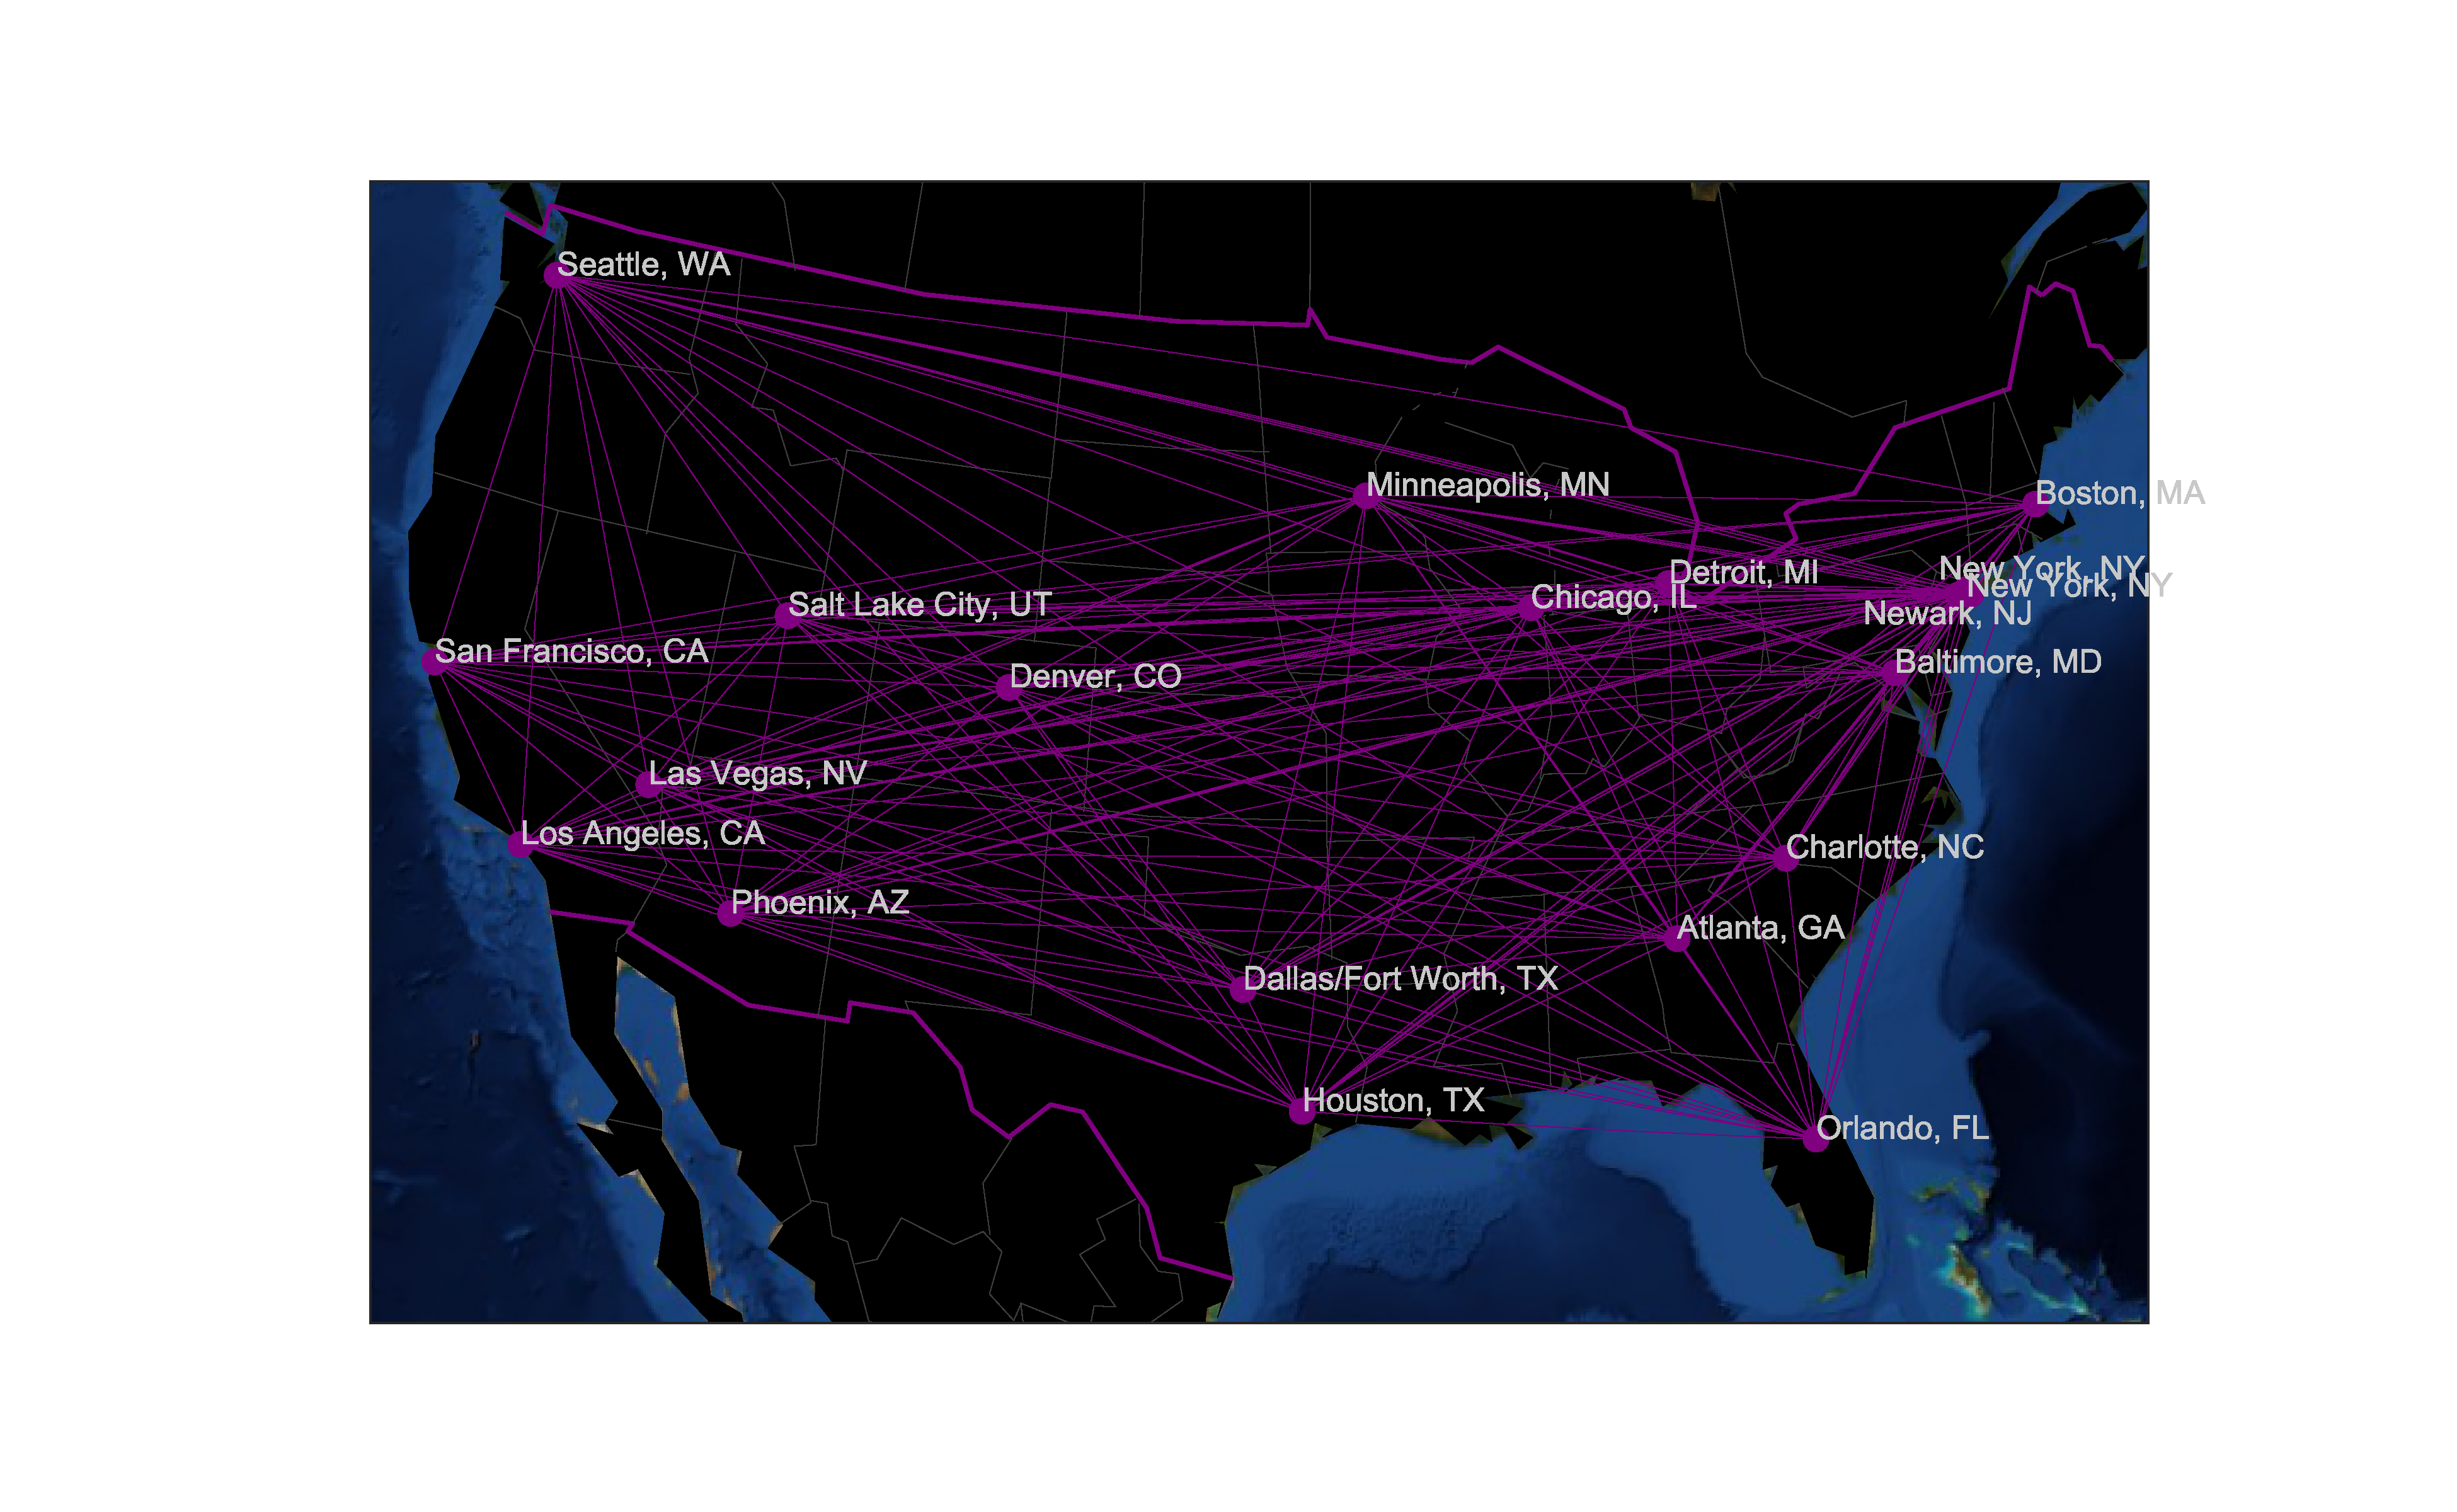
\includegraphics[width=6in]{map.pdf}
\end{center}
\caption{\label{fig:map}
Network of top 20 airports in the US. Note that there are two airports in the New York City: LGA and JFK.}
\end{figure}
The justification for selecting these 20 airports is discussed in detail in \href{https://github.com/aajains/springboard-datascience-intensive/blob/master/capstone_project/DataAcquisitionMerging/data_acquisition_merging.ipynb}{this IPython notebook}. 


We will go through most of the fields (or columns) in the dataset to explore their relationship with flight cancellation rate. Details about each field can be found in \href{https://www.transtats.bts.gov/Fields.asp?Table_ID=236}{the Bureau of Transportation Statistics} and \href{https://www.wunderground.com/weather/api/d/docs?d=resources/phrase-glossary}{the Wunderground} websites and some in \href{https://github.com/aajains/springboard-datascience-intensive/blob/master/capstone_project/DataAcquisitionMerging/history_calc.ipynb}{this IPython notebook} and \href{https://github.com/aajains/springboard-datascience-intensive/blob/master/capstone_project/DataCleaning/data_cleaning.ipynb}{this IPython notebook}. The target column for this project is called  "Cancelled" which contains two values: 1 for cancelled flights and 0 for not-cancelled flights. 
%%%%%%%%%%%%%%%%%%%%%%%%%
\subsection{Flight Cancellation Rate}
\label{subsec:canrate}
%%%%%%%%%%%%%%%%%%%%%%%%%
Out of 2.8$+$ million flights operating at top 20 airports in 2015-2016, about 1.15$\%$ of them got cancelled. This does not seem like a large number but such rare events cause a great deal of inconveniences to passengers, and cost a lot of money to airline companies. Therefore, it is important to understand where, when and how this small events occur. To start with, we plot the total number of flights on a daily basis and see how many flights got cancelled (on a daily basis) in Fig. \ref{fig:daily}. 
\begin{figure}[h!]
\begin{center}
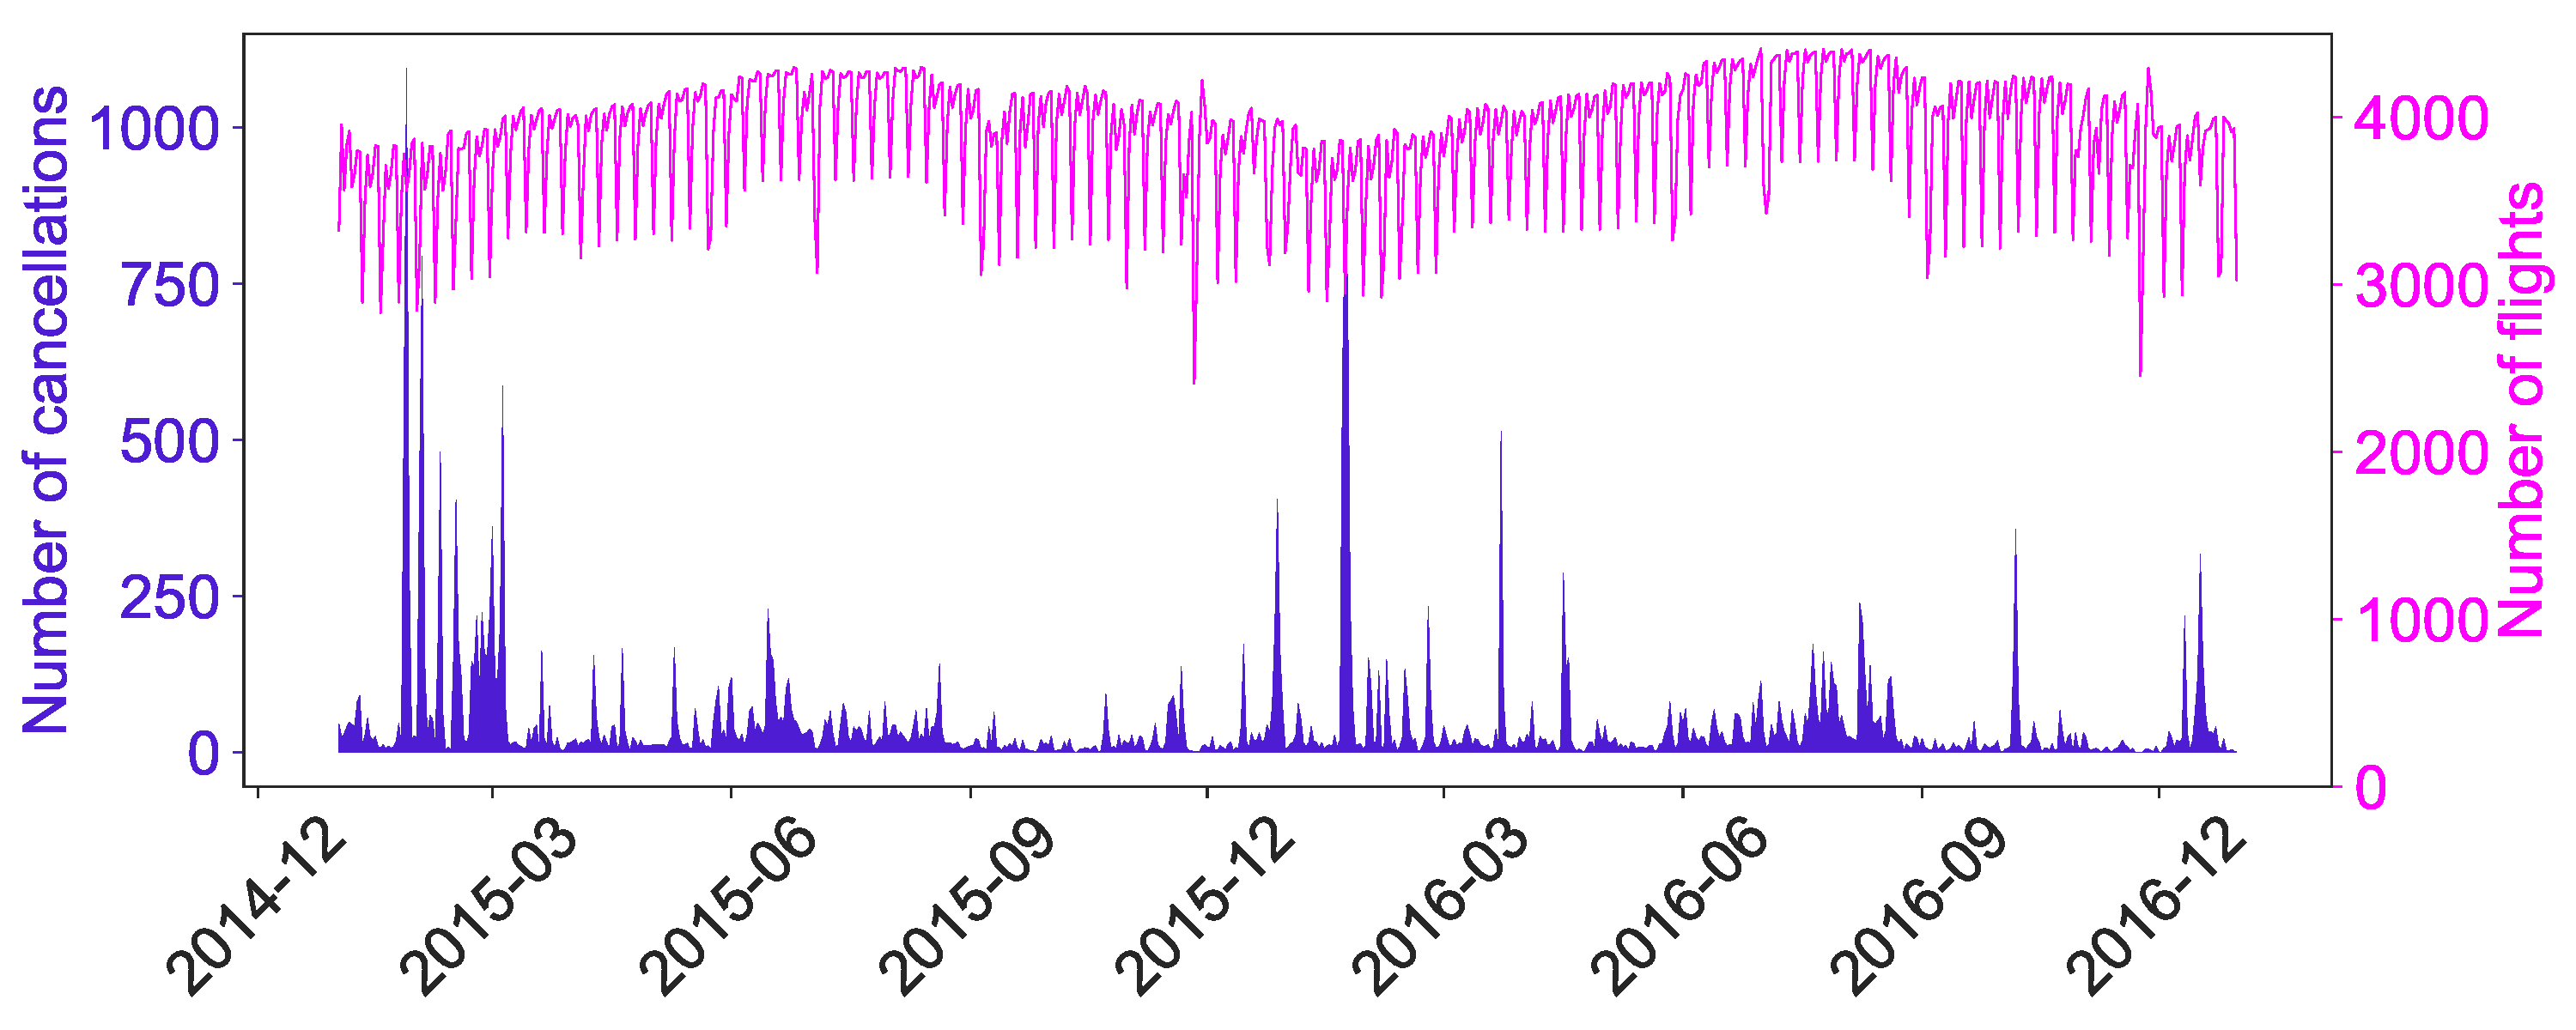
\includegraphics[width=6in]{daily_flights_cancellations.pdf}
\end{center}
\caption{\label{fig:daily}
Total number of flights (right y-axis) and number of cancelled flights (left y-axis), on a daily basis.}
\end{figure}
The daily total number of flights remain almost steady with regular and periodic troughs. The number of cancelled flights has no steady trend but has some big spikes. Knowing the number of flights and number of cancellations, we can calculate the cancellation rate for a given day. We define the cancellation rate as, 
\begin{equation}
\label{eq:canrate}
\text{Flight cancellation rate} = \frac{\text{Number of flights cancelled for a given scenario}}{\text{Total number of flights for a given scenario}},
\end{equation}
where a ``scenario" can refer to a class of a field. In the plot above, a scenario would refer to a date, say June 24th 2015. Figure \ref{fig:dailycanrate} shows the daily $\%$ cancellation rates.  
\begin{figure}[h!]
\begin{center}
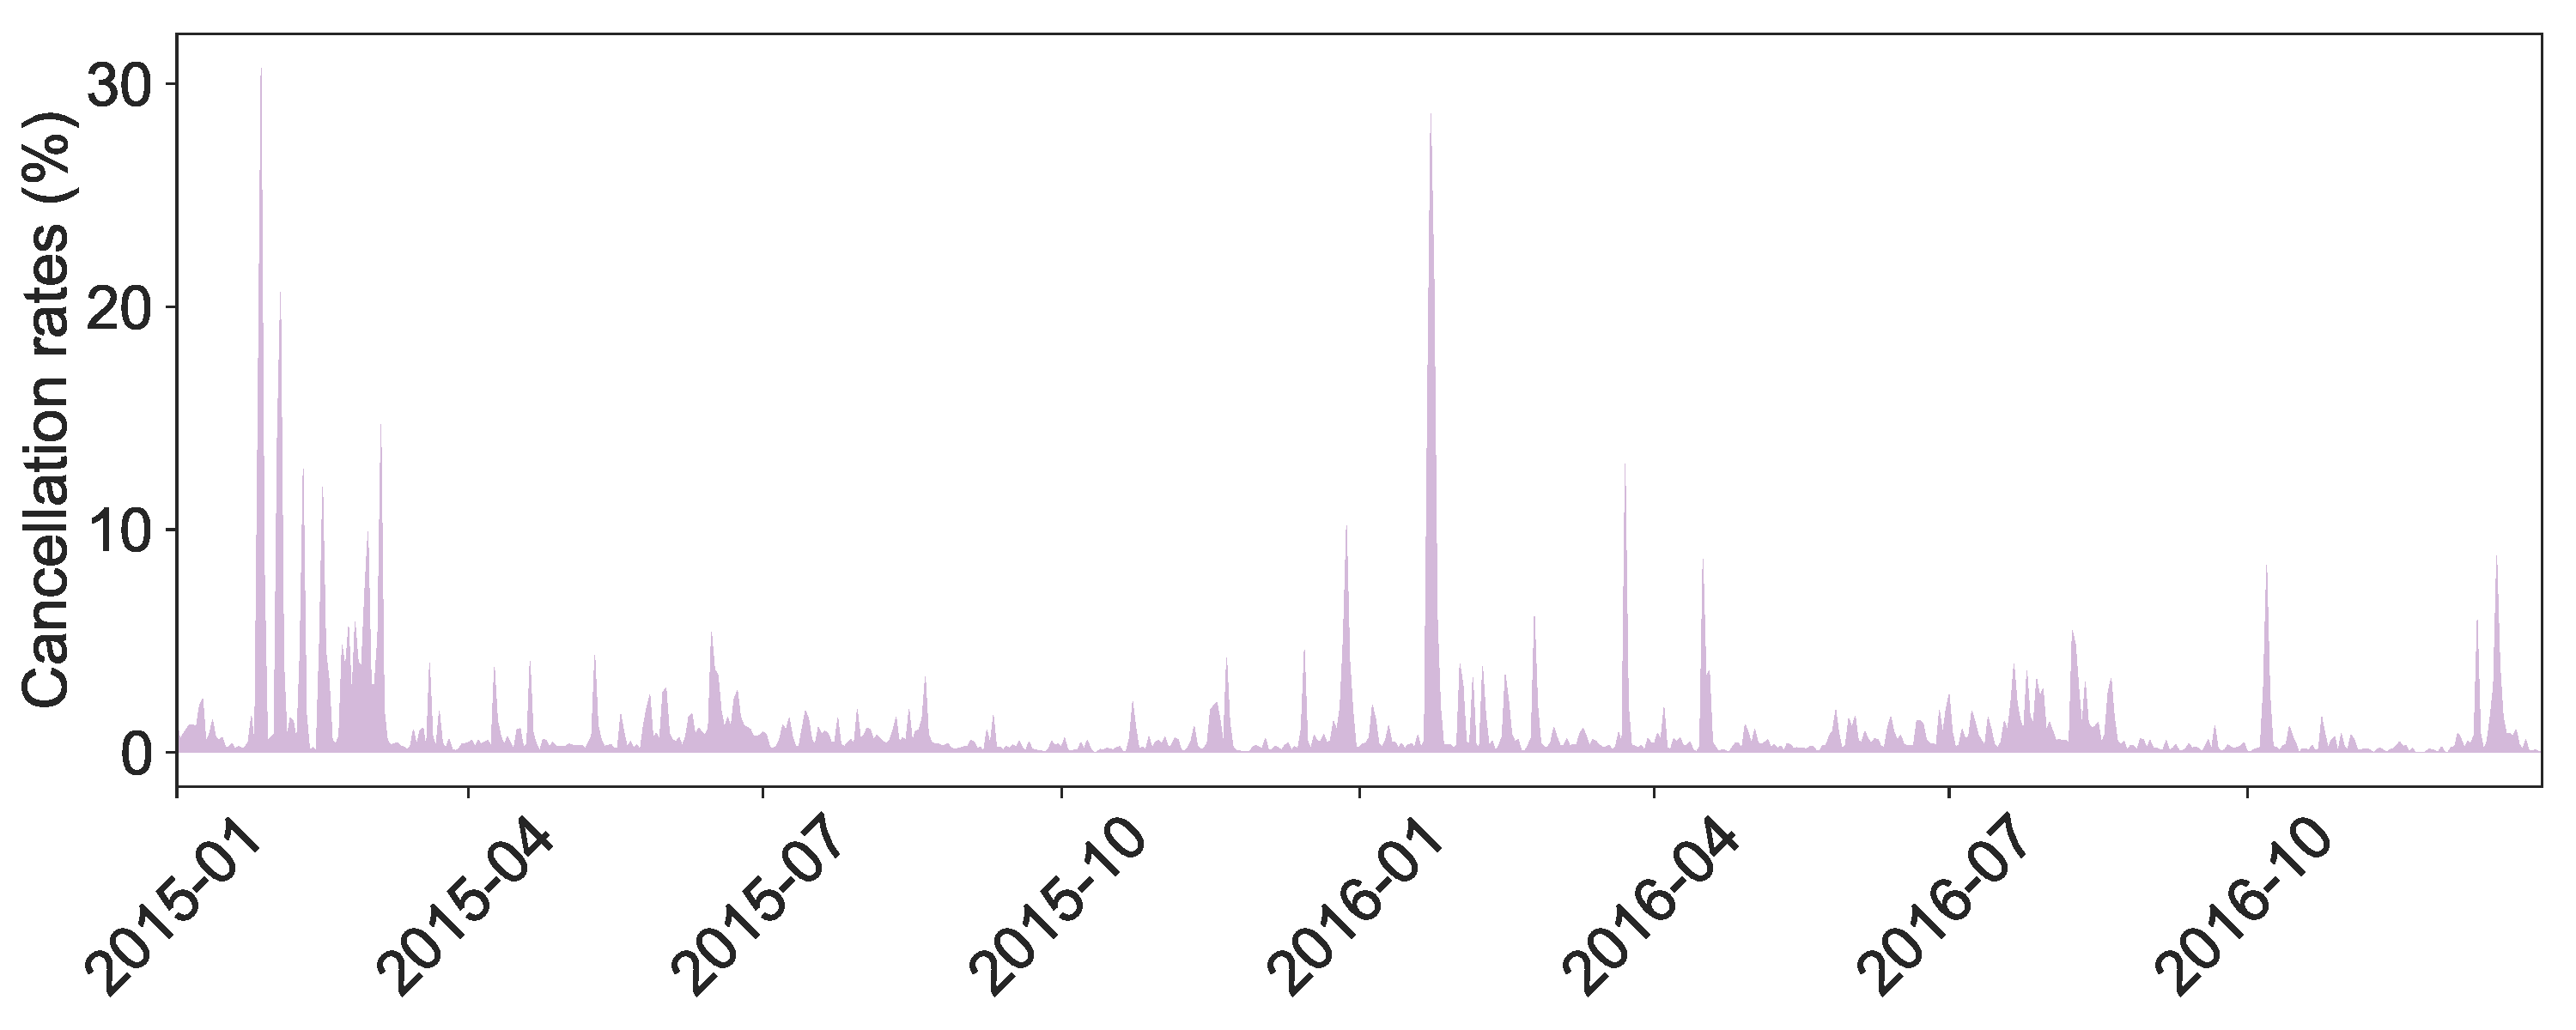
\includegraphics[width=6in]{daily_canrate.pdf}
\end{center}
\caption{\label{fig:dailycanrate}
Daily cancellation rates.}
\end{figure}
Big spikes in the cancellation rates were mainly caused by bad weather as depicted above. There were some spikes in cancellation activities in the end of June and beginning of December too.


We can discuss some other examples for cancellation rates also. For instance, if the field is weather condition which has classes such as Heavy Snow, Rain, Clear Sky etc.., a scenario can be one of these weather conditions. We then count the number of flights operating under such a scenario (say Heavy Snow) and also count the number of flights that got cancelled under the same scenario. Equation~(\ref{eq:canrate}) can then be used to calculate the cancellation rate when the weather condition is Heavy Snow. In the following few sub-sections, we will go through many interesting fields and explore the trend for cancellation rates. There are broadly 6 categories of information that are embedded in all the fields: 
\begin{enumerate}
\itemsep0em
\item Calendar variables
\item Airports
\item Airlines
\item Flight distance
\item Weather factors
\item Historical performances 
\end{enumerate}
%%%%%%%%%%%%%%%%%%%%%%%%%
\subsection{Calendar Variables}
\label{subsec:calvar}
%%%%%%%%%%%%%%%%%%%%%%%%%
There are many calendar variables such as quarter, month, week, day, hour, minute, etc.. Here, we explore the dependency of cancellation rates on month, day of week and scheduled hour. For some flights the origin and destination calendar variables can be different, and hence we calculate the cancellation rates for all variables at both origin and destination airports. Figure \ref{fig:monthlycanrate} shows the monthly cancellation rate.  
\begin{figure}[h!]
\begin{center}
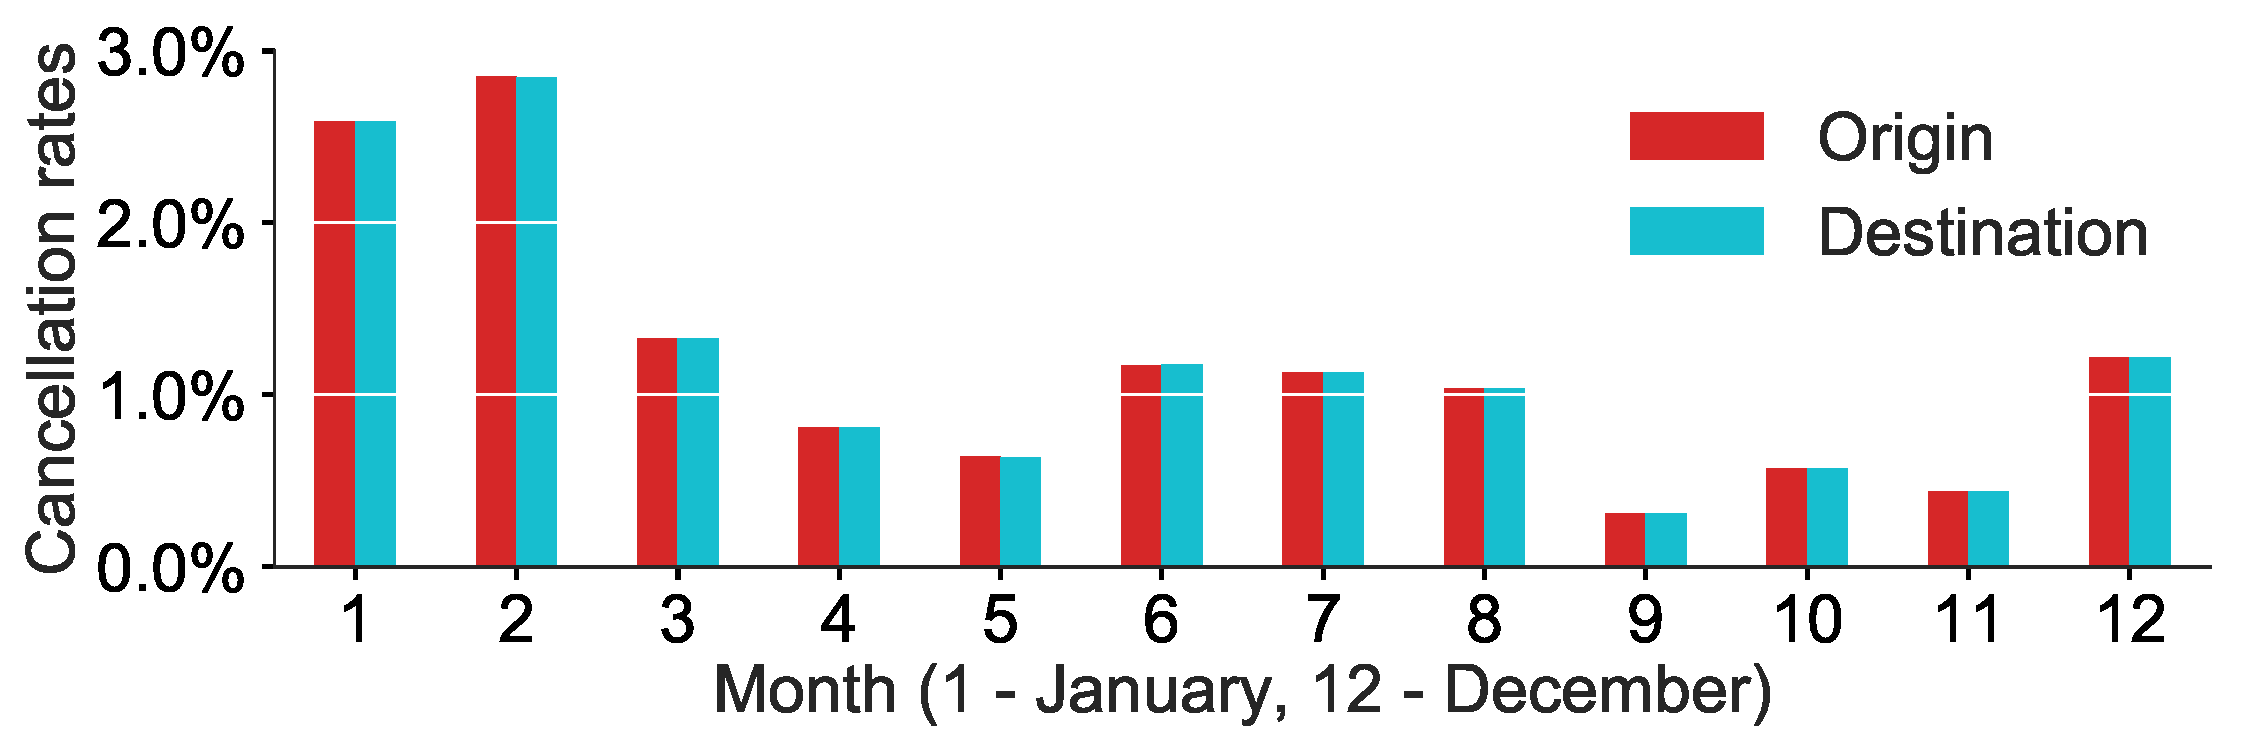
\includegraphics[width=6in]{monthly_canrate.pdf}
\end{center}
\caption{\label{fig:monthlycanrate}
Monthly cancellation rates.}
\end{figure}
There is no difference in cancellation rates between the origin and the destination airports in any given month. February was the worst followed by January and March. We see some mild spikes for June and December too. The high cancellation rate in January and February was mainly due to the snow storms in the east coast. We can also look at the day of the week and understand its influence on the cancellation rate in Fig. \ref{fig:weeklycanrate}. 
\begin{figure}[h!]
\begin{center}
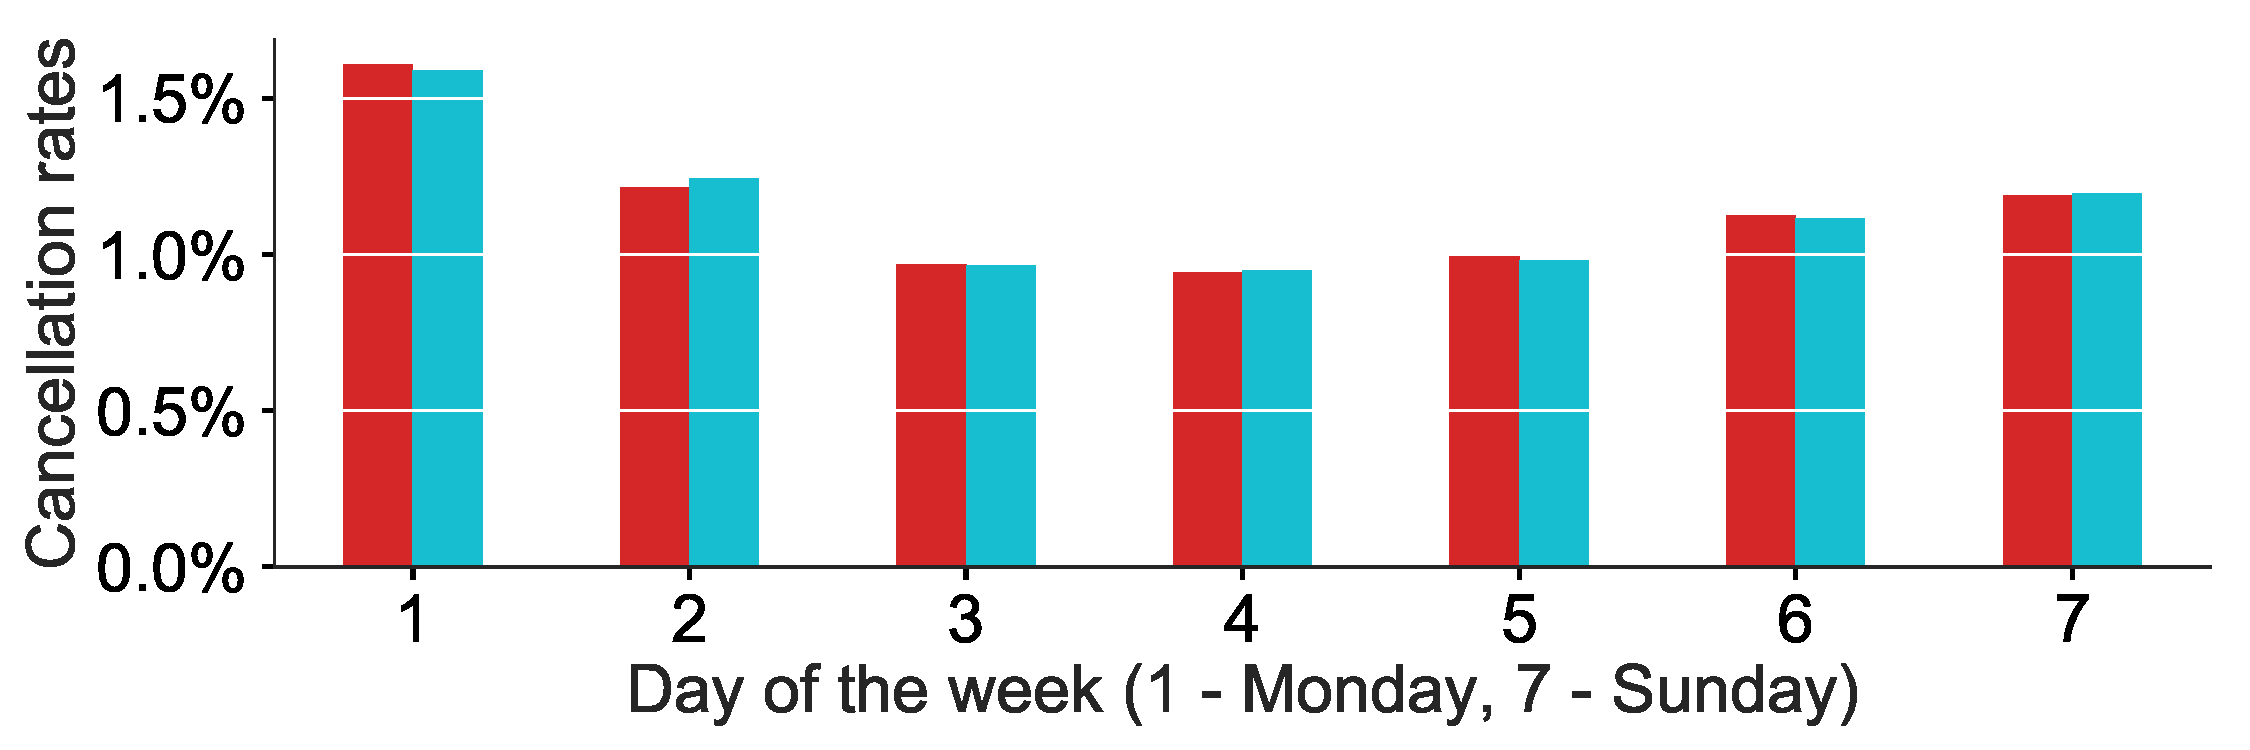
\includegraphics[width=6in]{weekly_canrate.pdf}
\end{center}
\caption{\label{fig:weeklycanrate}
Cancellation rates depend on the day of the week. Note the colors correspond to the same legend as in Fig.\ref{fig:monthlycanrate}.}
\end{figure}
End of the weekend and beginning of the week observed higher cancellation rates as compared to the middle week days. There are very slight differences in cancellation rates between the origin and the destination airports for any day of the week. We can go down one more level in the calendar variable space and explore the hours of the flights throughout the day in Fig. \ref{fig:hourlycanrate}.
\begin{figure}[h!]
\begin{center}
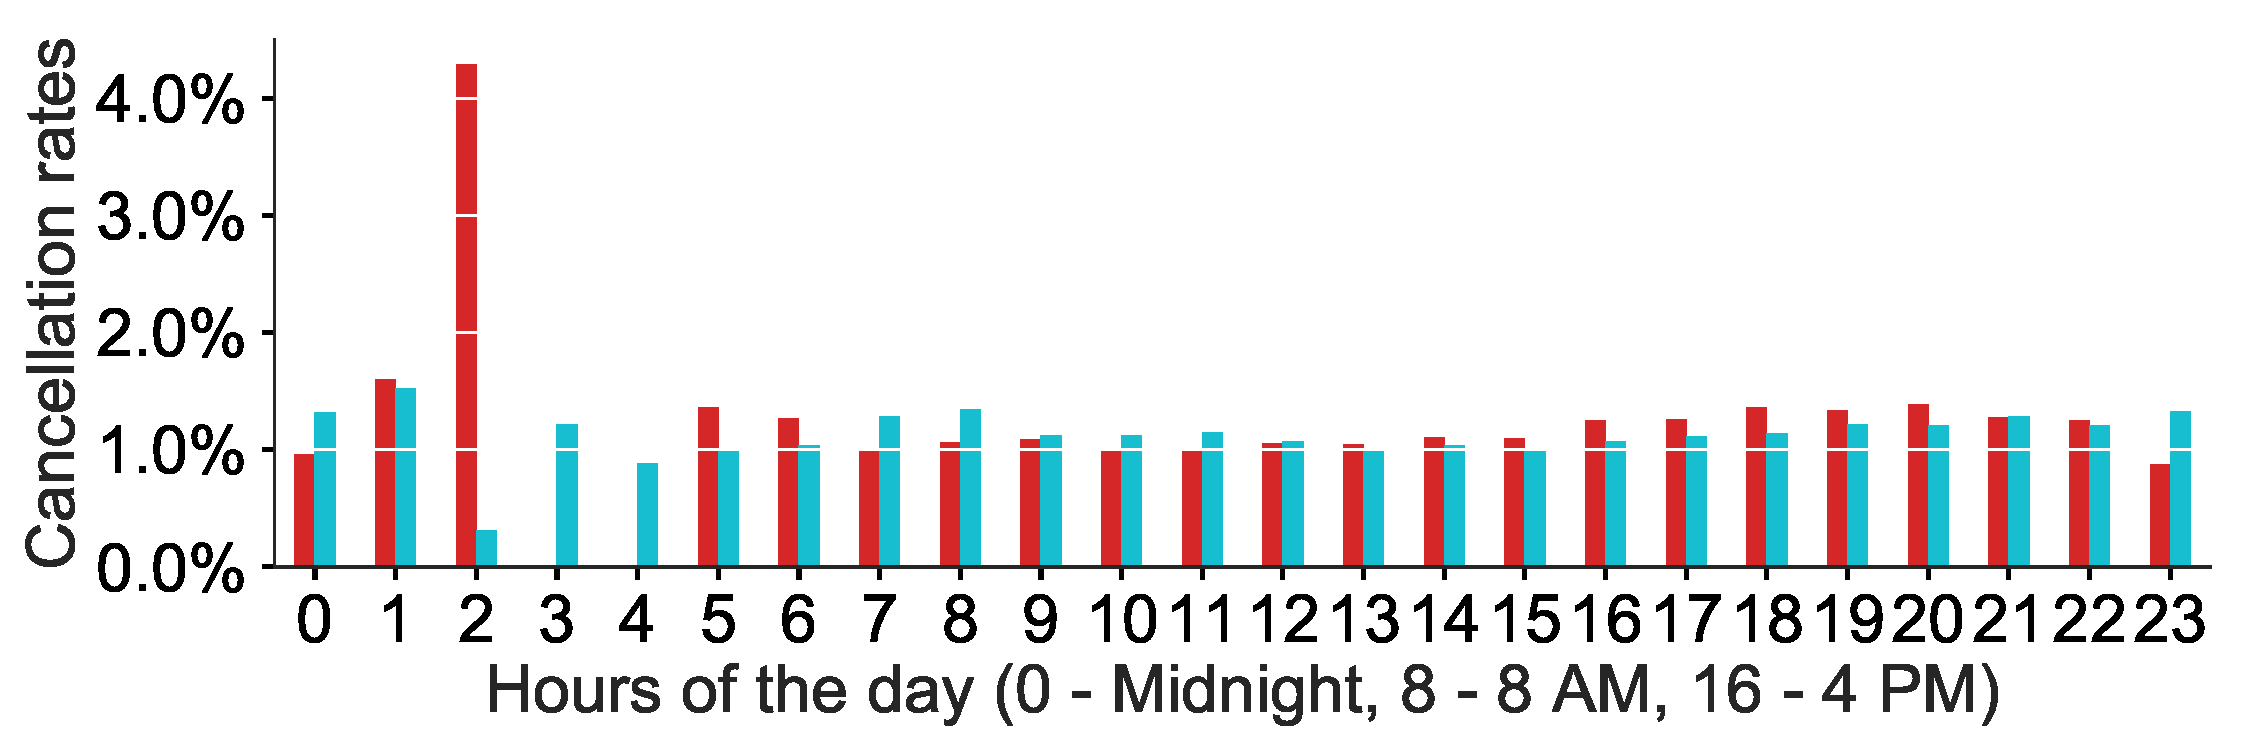
\includegraphics[width=6in]{hourly_canrate.pdf}
\end{center}
\caption{\label{fig:hourlycanrate}
Hourly cancellation rates throughout the day. Note the colors correspond to the same legend as in Fig.\ref{fig:monthlycanrate}.}
\end{figure}
For all scheduled departure hours, except between 2 - 3 AM, the cancellation rates are below $2\%$. We do not see any big spike in the case of scheduled arrival hours. Out of 210 flights scheduled to depart between 2-3 AM , 9 were cancelled, leading to spike at 2-3 AM red bar in the figure. This completes our brief discussion on calendar variables.
%%%%%%%%%%%%%%%%%%%%%%%%%
\subsection{Airports}
\label{subsec:airports}
%%%%%%%%%%%%%%%%%%%%%%%%%
We calculate the cancellation rates for flights departing from and arriving at all top 20 airports and display the results in Fig. \ref{fig:airportcanrate}. 
\begin{figure}[h!]
\begin{center}
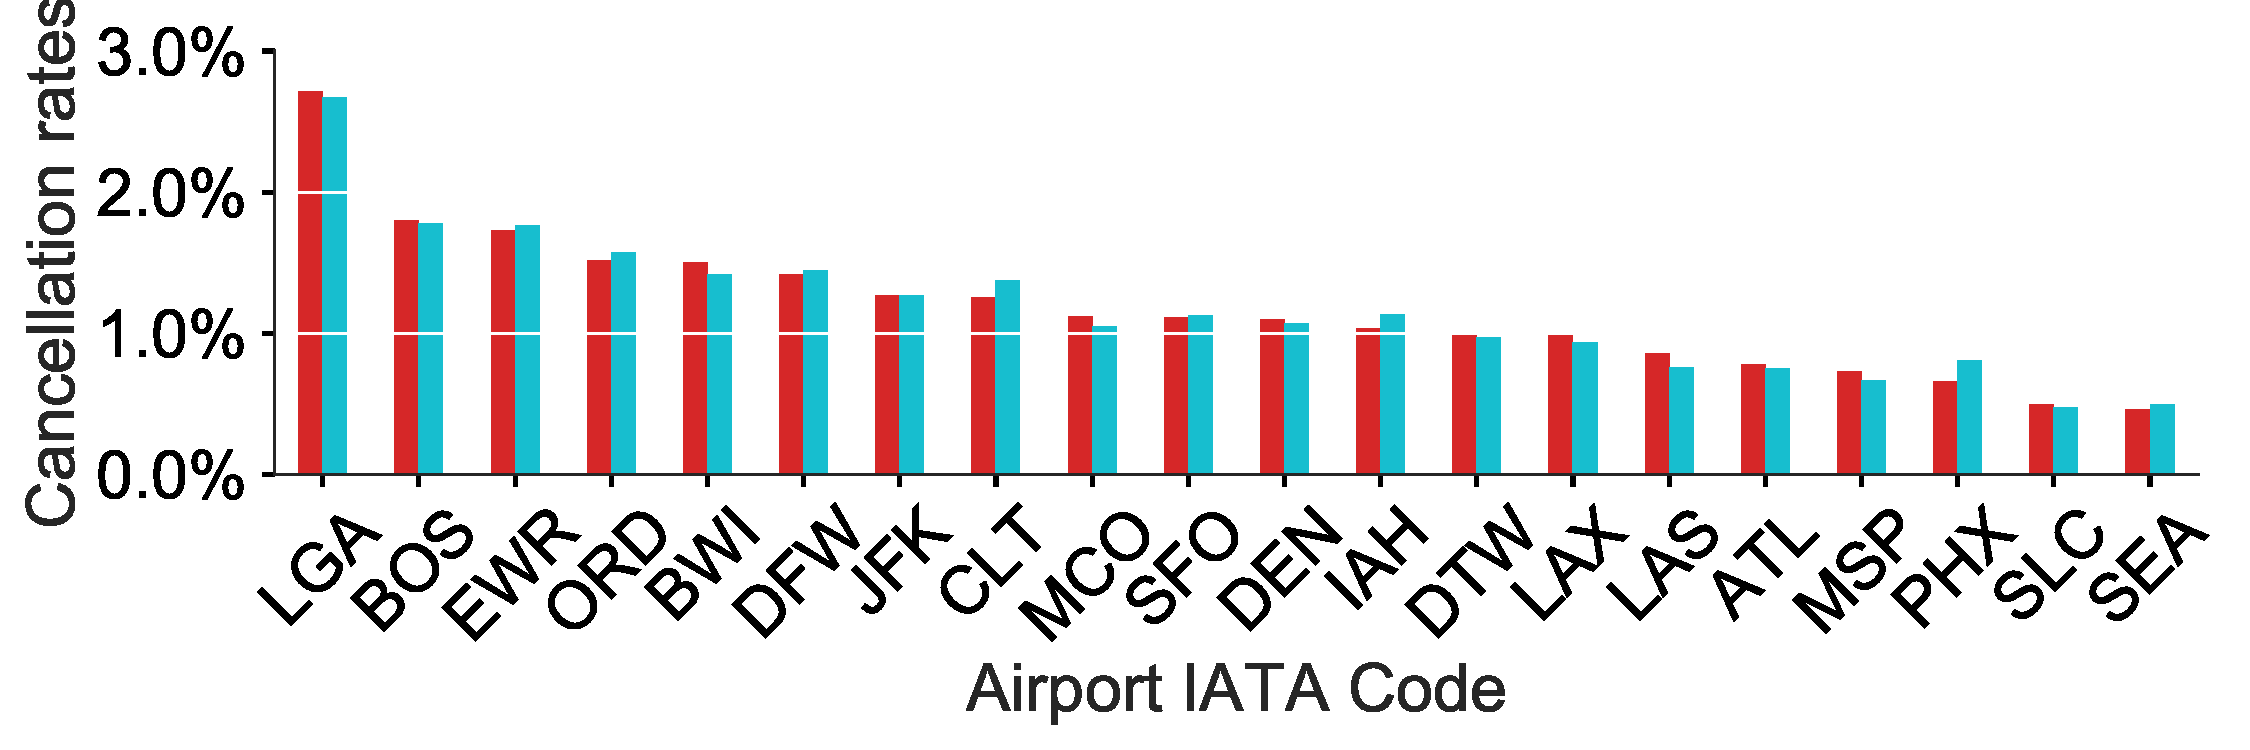
\includegraphics[width=6in]{airport_canrate.pdf}
\end{center}
\caption{\label{fig:airportcanrate}
Cancellation rates dependency on the airport. Note the colors correspond to the same legend as in Fig.\ref{fig:monthlycanrate}.}
\end{figure}
The IATA code can be found in \href{http://www.iata.org/publications/Pages/code-search.aspx}{this link}.
The flights departing from LaGuardia Airport (LGA) have the highest cancellation rate whereas the flights departing from Seattle - Tacoma International Airport (SEA) have lowest rate. The top 2 and the bottom 2 airports remain the same whether we are looking at origin or destination airport. 
%%%%%%%%%%%%%%%%%%%%%%%%%
\subsection{Airlines}
\label{subsec:airlines}
%%%%%%%%%%%%%%%%%%%%%%%%%
For airlines, it does not make sense to distinguish between the origin and destination. Figure \ref{fig:airlinecanrate} shows the cancellation rates for 13 airlines.  
\begin{figure}[h!]
\begin{center}
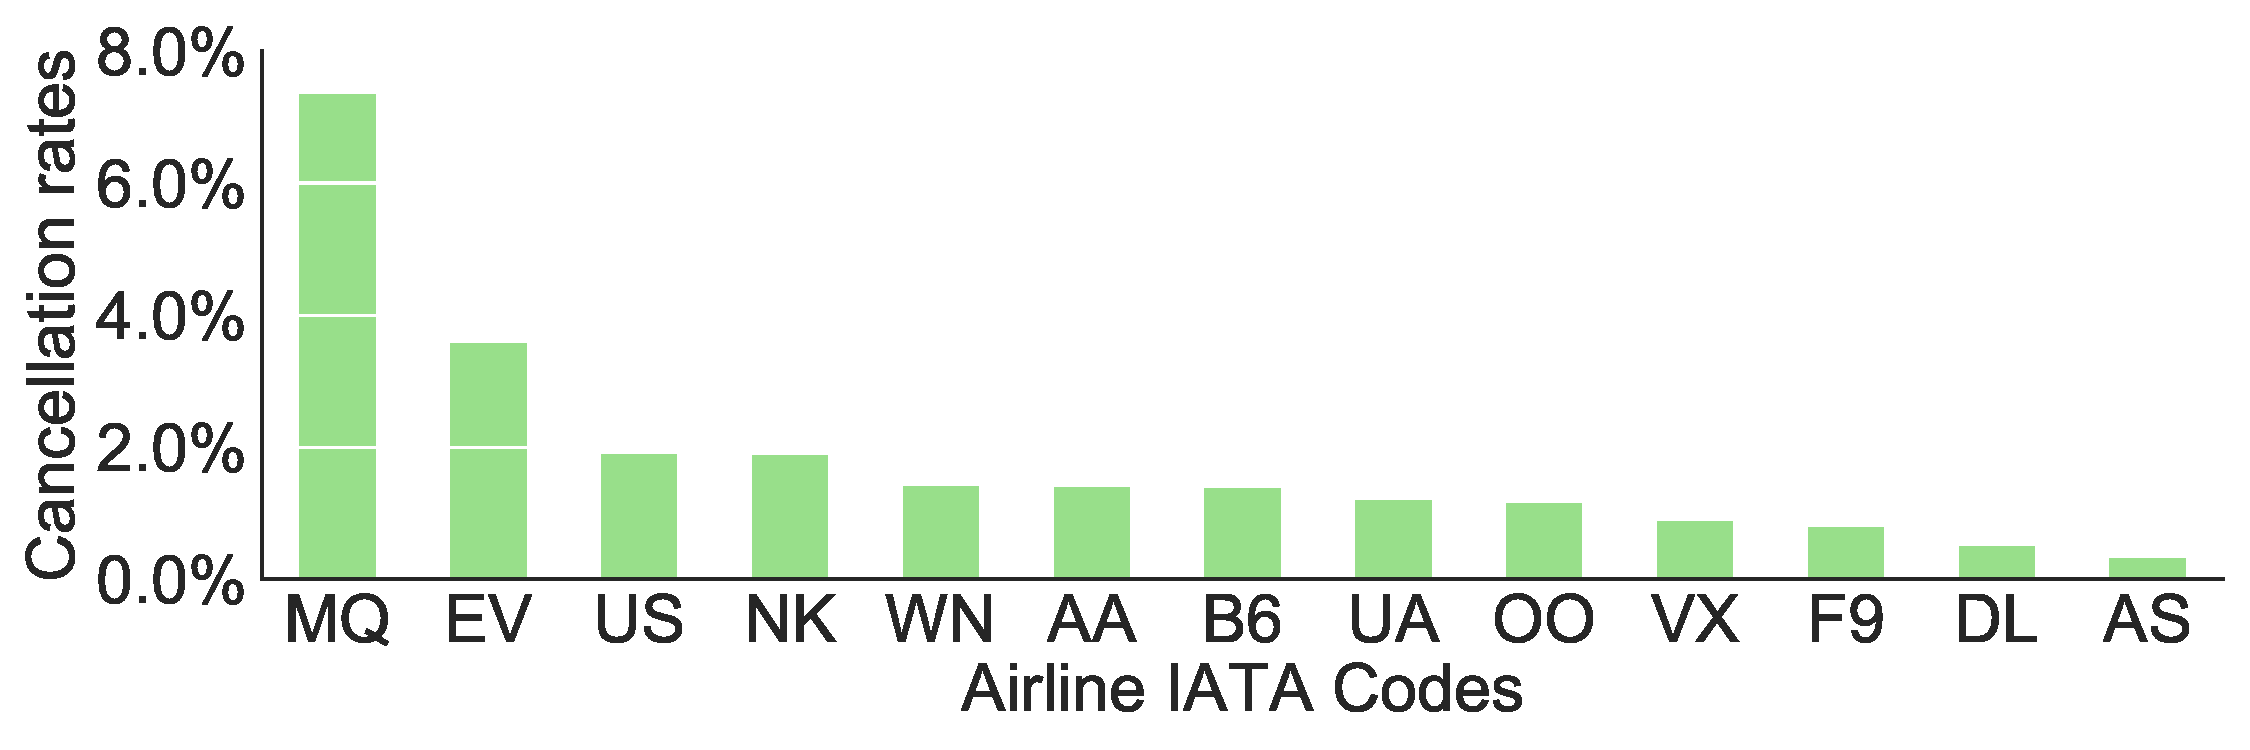
\includegraphics[width=6in]{airline_canrate.pdf}
\end{center}
\caption{\label{fig:airlinecanrate}
Cancellation rates dependency on the airline.}
\end{figure}
The airline IATA code can be found in \href{http://www.iata.org/publications/Pages/code-search.aspx}{this link}. The highest cancellation rate is seen for the Envoy Air (MQ), and lowest is seen for the Alaska Airlines (AS). Two airlines with highest cancellation rates (MQ and EV) are not mainline airlines but rather regional ones. OO (SkyWest Airlines) is also regional airline but has relatively lower cancellation rates.
%%%%%%%%%%%%%%%%%%%%%%%%%
\subsection{Flight Distance}
\label{subsec:flightdistance}
%%%%%%%%%%%%%%%%%%%%%%%%%
Flight distance is recorded in miles and is a continuous variable. For every numerical value of this variable, we calculate the cancellation rate, which is shown in Fig. \ref{fig:distancecanrate}.   
\begin{figure}[h!]
\begin{center}
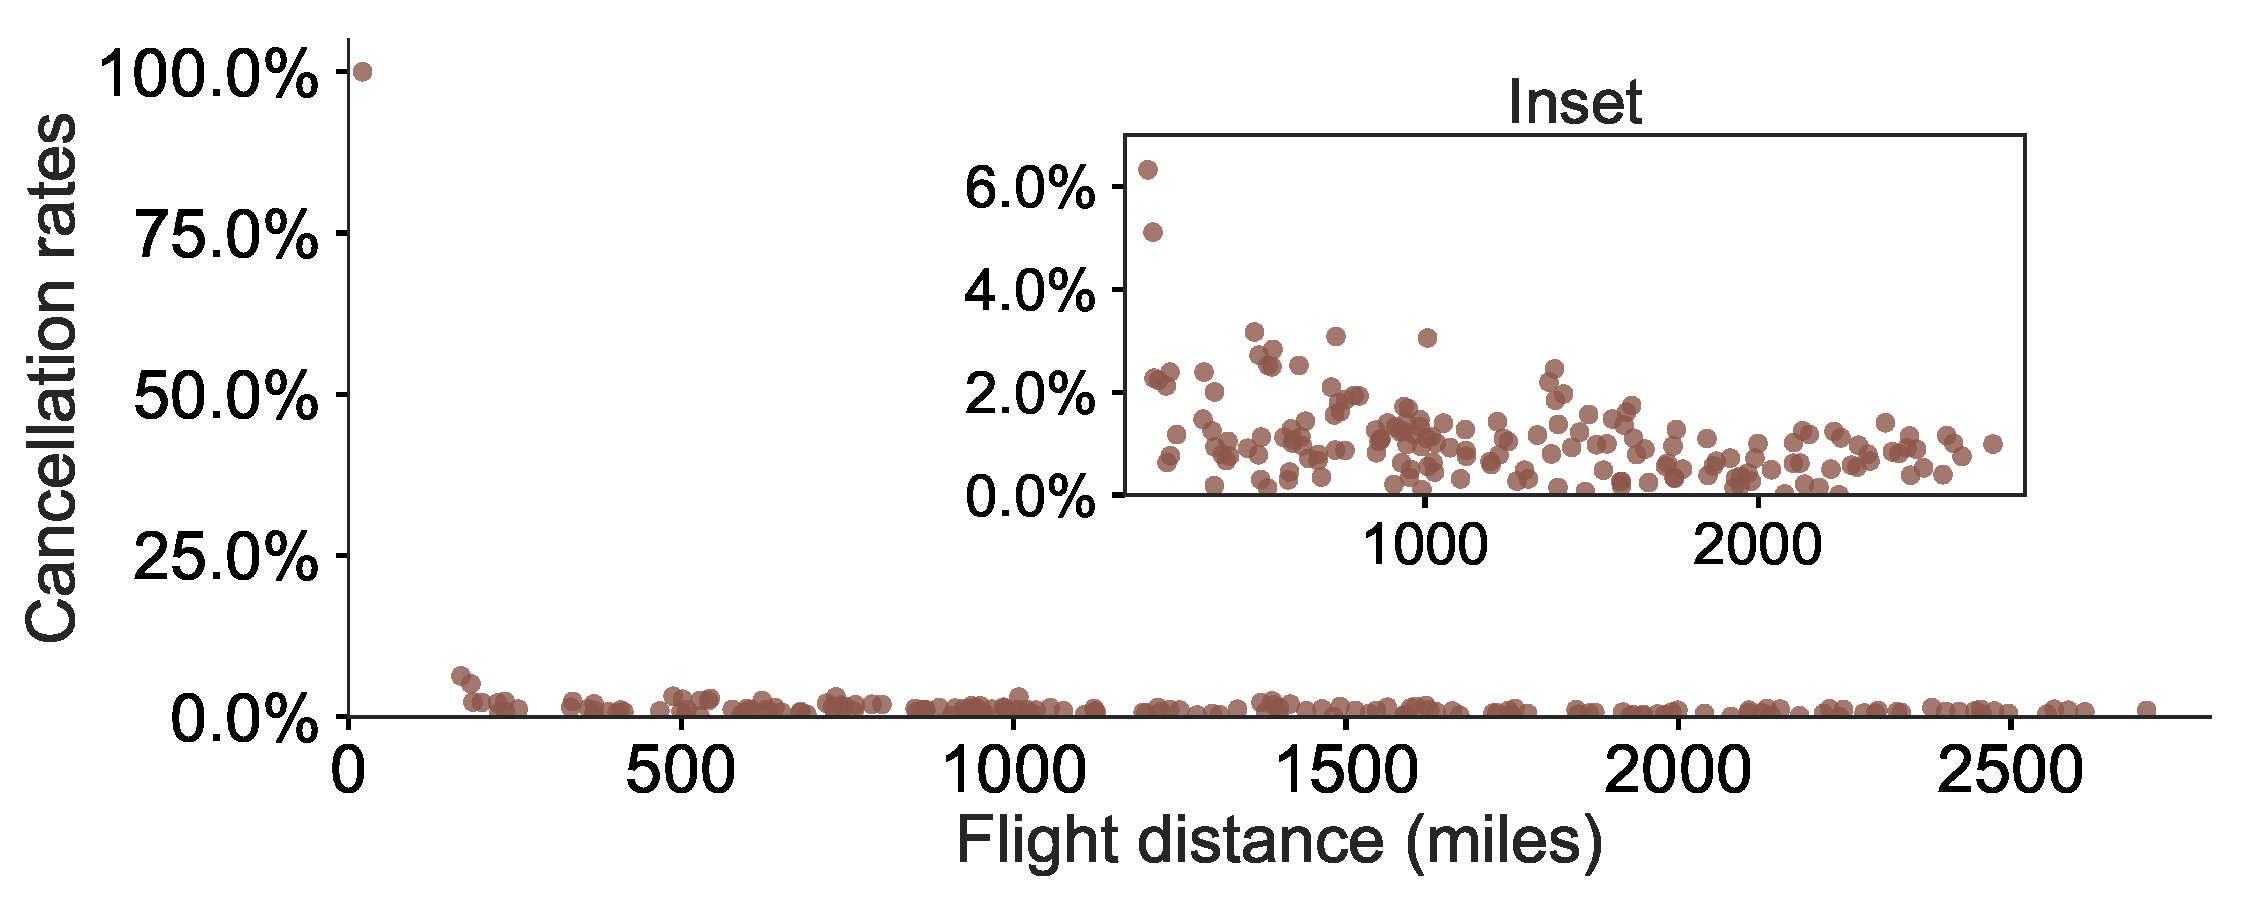
\includegraphics[width=6in]{distance_canrate.pdf}
\end{center}
\caption{\label{fig:distancecanrate}
Cancellation rates as a function of flight distance.}
\end{figure}
There is a data point for Distance = 21 miles for which the cancellation rate was 100$\%$. In order to see the clear trend for all other data points, we omitted the 21 miles point and replotted the data in the inset figure. We can see that the cancellation rates are higher for shorter distance flights and lower for longer distance flights. We performed a hypothesis test to test the null that there is no relationship between the distance and the cancellation rate. Using Spearman's $\rho$, we found a weak correlation of -0.39 which was statistically significant. 
%%%%%%%%%%%%%%%%%%%%%%%%%
\subsection{Weather Factors}
\label{subsec:weatherfactors}
%%%%%%%%%%%%%%%%%%%%%%%%%
There are many weather factors such as temperature, dew point, pressure, wind speed, wind direction, humidity etc.. but we will focus on only some factors here to keep the discussion short. A detailed data exploration can be found in \href{https://github.com/aajains/springboard-datascience-intensive/blob/master/capstone_project/EDA/ExploratoryDataAnalysis.ipynb}{this IPython notebook}. 


Fig. \ref{fig:tempcanrate} displays the cancellation rate asa function of temperature at both origin and destination (at the time of departure and arrival, respectively). There appears to be two broad temperature regimes here in terms of cancellation rates. The cancellation rates are four times higher when the temperatures are below 40 $^\circ$F as compared to the situations when temperatures above 40 $^\circ$F. which can be clearly seen in the inset figure. 
\begin{figure}[h!]
\begin{center}
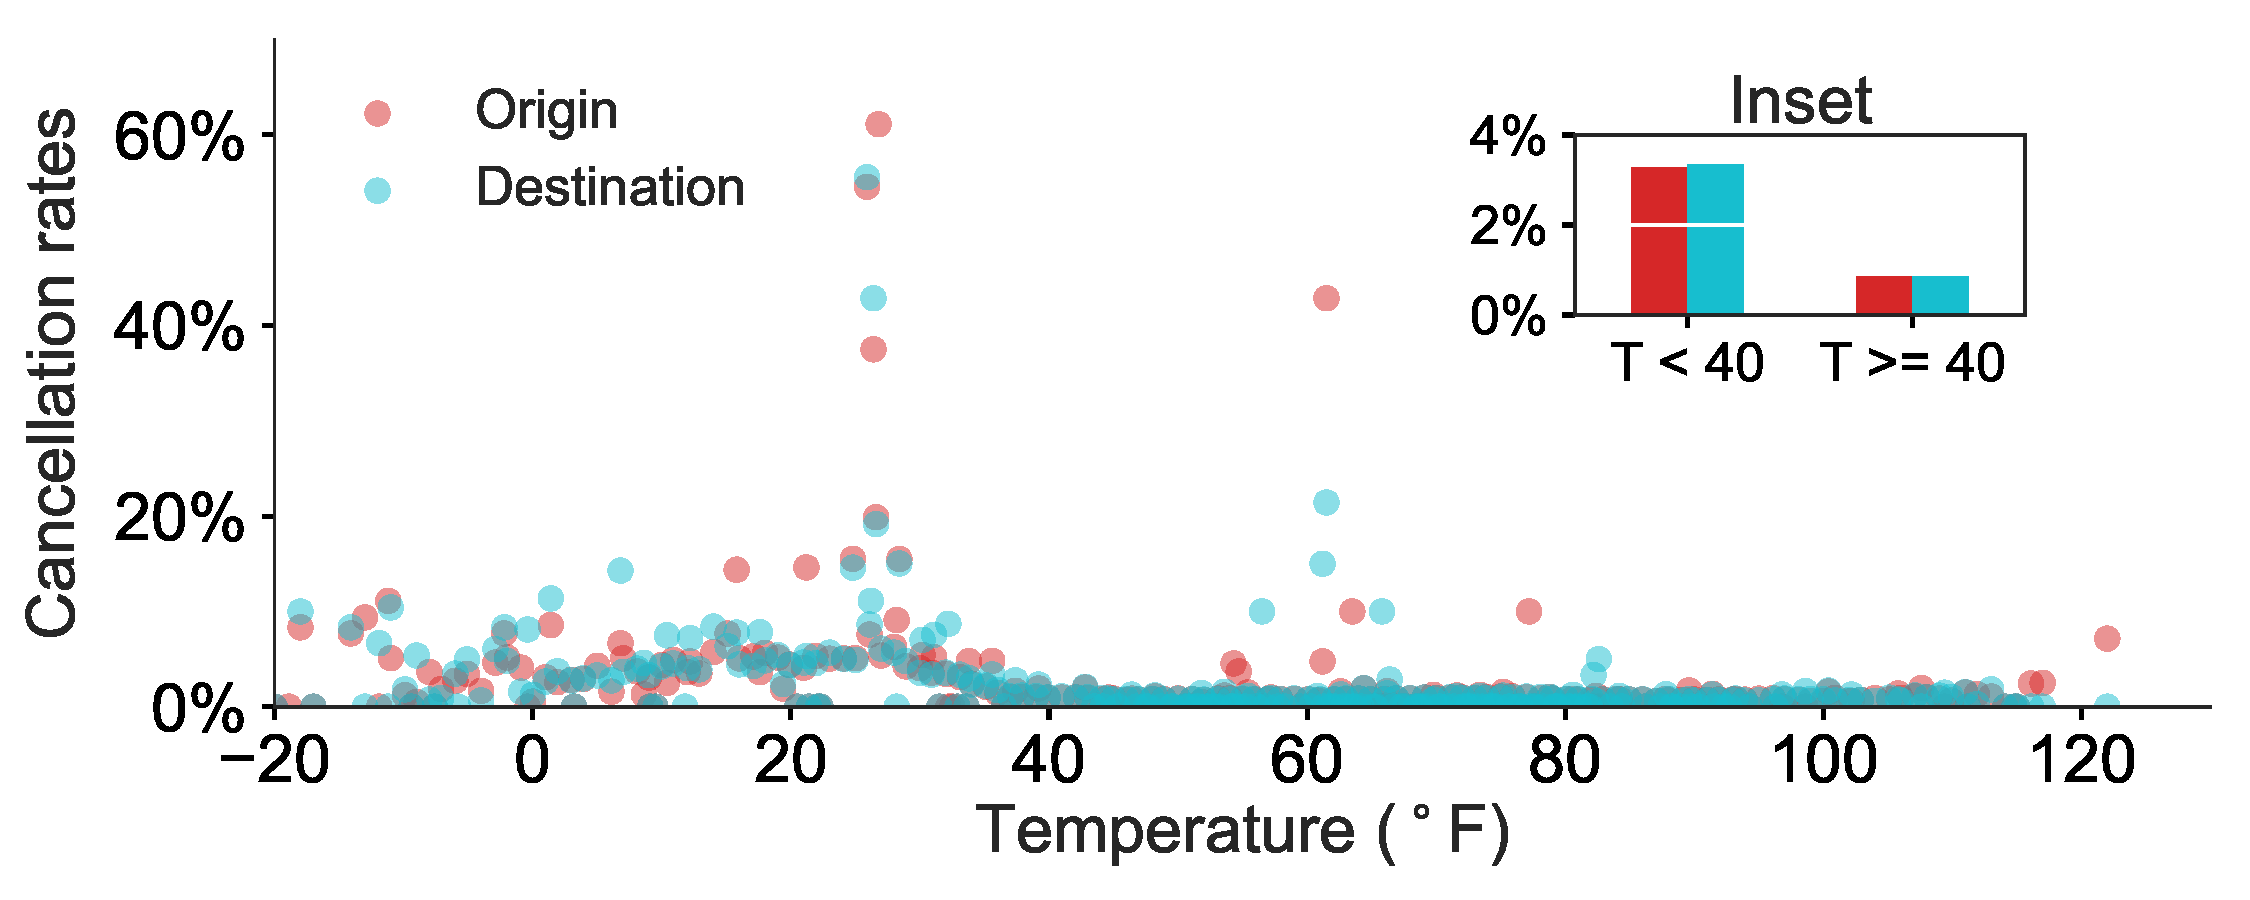
\includegraphics[width=6in]{temperature_canrate.pdf}
\end{center}
\caption{\label{fig:tempcanrate}
Cancellation rate as a function of temperature. In the inset bar chart, y-axis is for the cancellation rate and $T$ represents temperature.}
\end{figure}
Humidity and wind speed have similar effects on cancellation rates as shown in Fig. \ref{fig:humwindcanrate} for both origin and destination locations. For very dry weather conditions (less than 10$\%$), there is a decreasing trend for cancellation rate. The rate then monotonically increase for humidity more than 20$\%$. For the monotonic part, we found statistically significant values of Spearman's correlation $\rho$ to be around 0.79 for origin and 0.82 for destination. 
\begin{figure}[h!]
\begin{center}
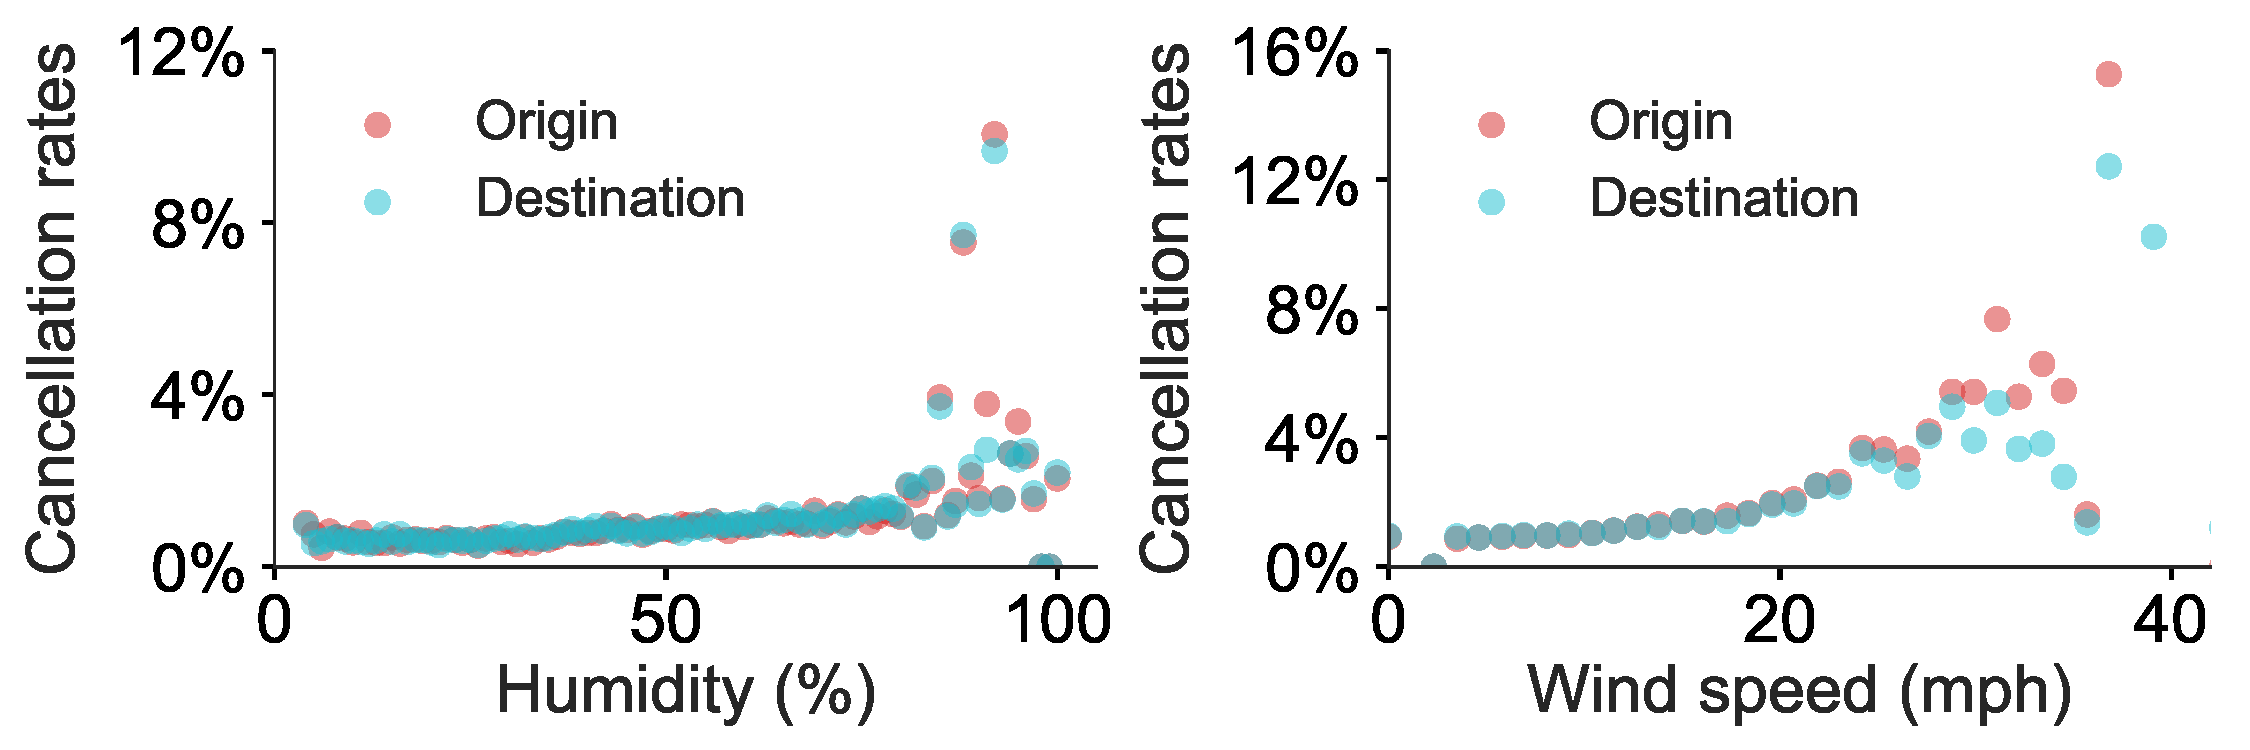
\includegraphics[width=6in]{humidity_windspeed_canrate.pdf}
\end{center}
\caption{\label{fig:humwindcanrate}
Cancellation rate as a function of $\%$ humidity and wind speed (mph).}
\end{figure}
Also, we see a monotonically increasing trend for cancellation rates as a function of wind speed until around 25 mph. For wind speed greater than that, the cancellation rates start to decrease. The maximum point for cancellation rates are different for origin and destination airports. Overall, the trends are pretty much like parabolic curves for wind speed.


We now look at the wind direction in FIg. \ref{fig:winddircanrate}. It turns out that from 90 to 270 degrees, i.e. from East to South to West, the cancellation rates are around 1$\%$. When the wind direction goes from West to close to North, the cancellation rates increased. The rates fluctuate a lot when the wind direction is close to North. From North to Wast wind direction, the cancellation rate start to decrease.
\begin{figure}[h!]
\begin{center}
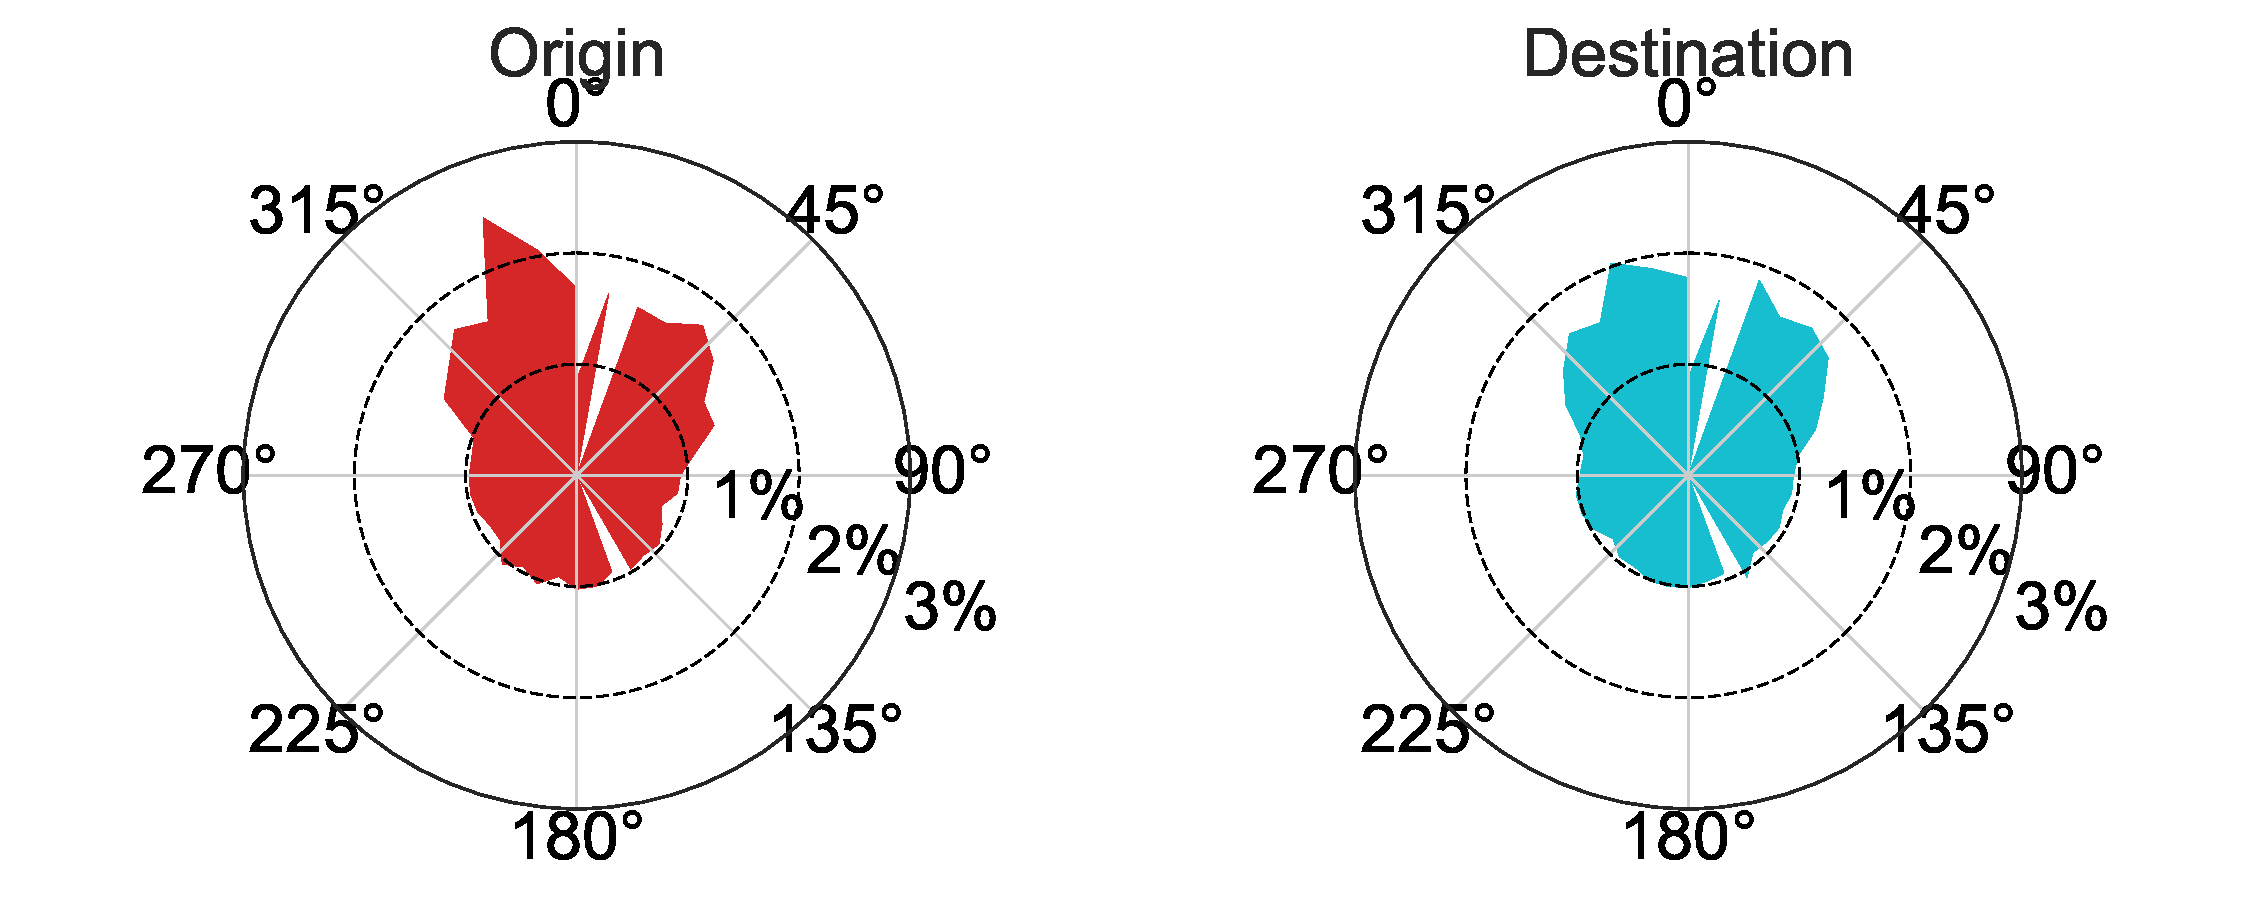
\includegraphics[width=6in]{winddir_canrate.pdf}
\end{center}
\caption{\label{fig:winddircanrate}
Cancellation rate as a function of wind direction. 0$^\circ$ corresponds to North, 90$^\circ$$\%$ to East, 180$^\circ$ to South and 270$^\circ$ to West.}
\end{figure}
Finally, we look at various weather conditions and find out the cancellation rates under all conditions, as displayed in Fig. \ref{fig:conditionscanrate}.
\begin{figure}[h!]
\begin{center}
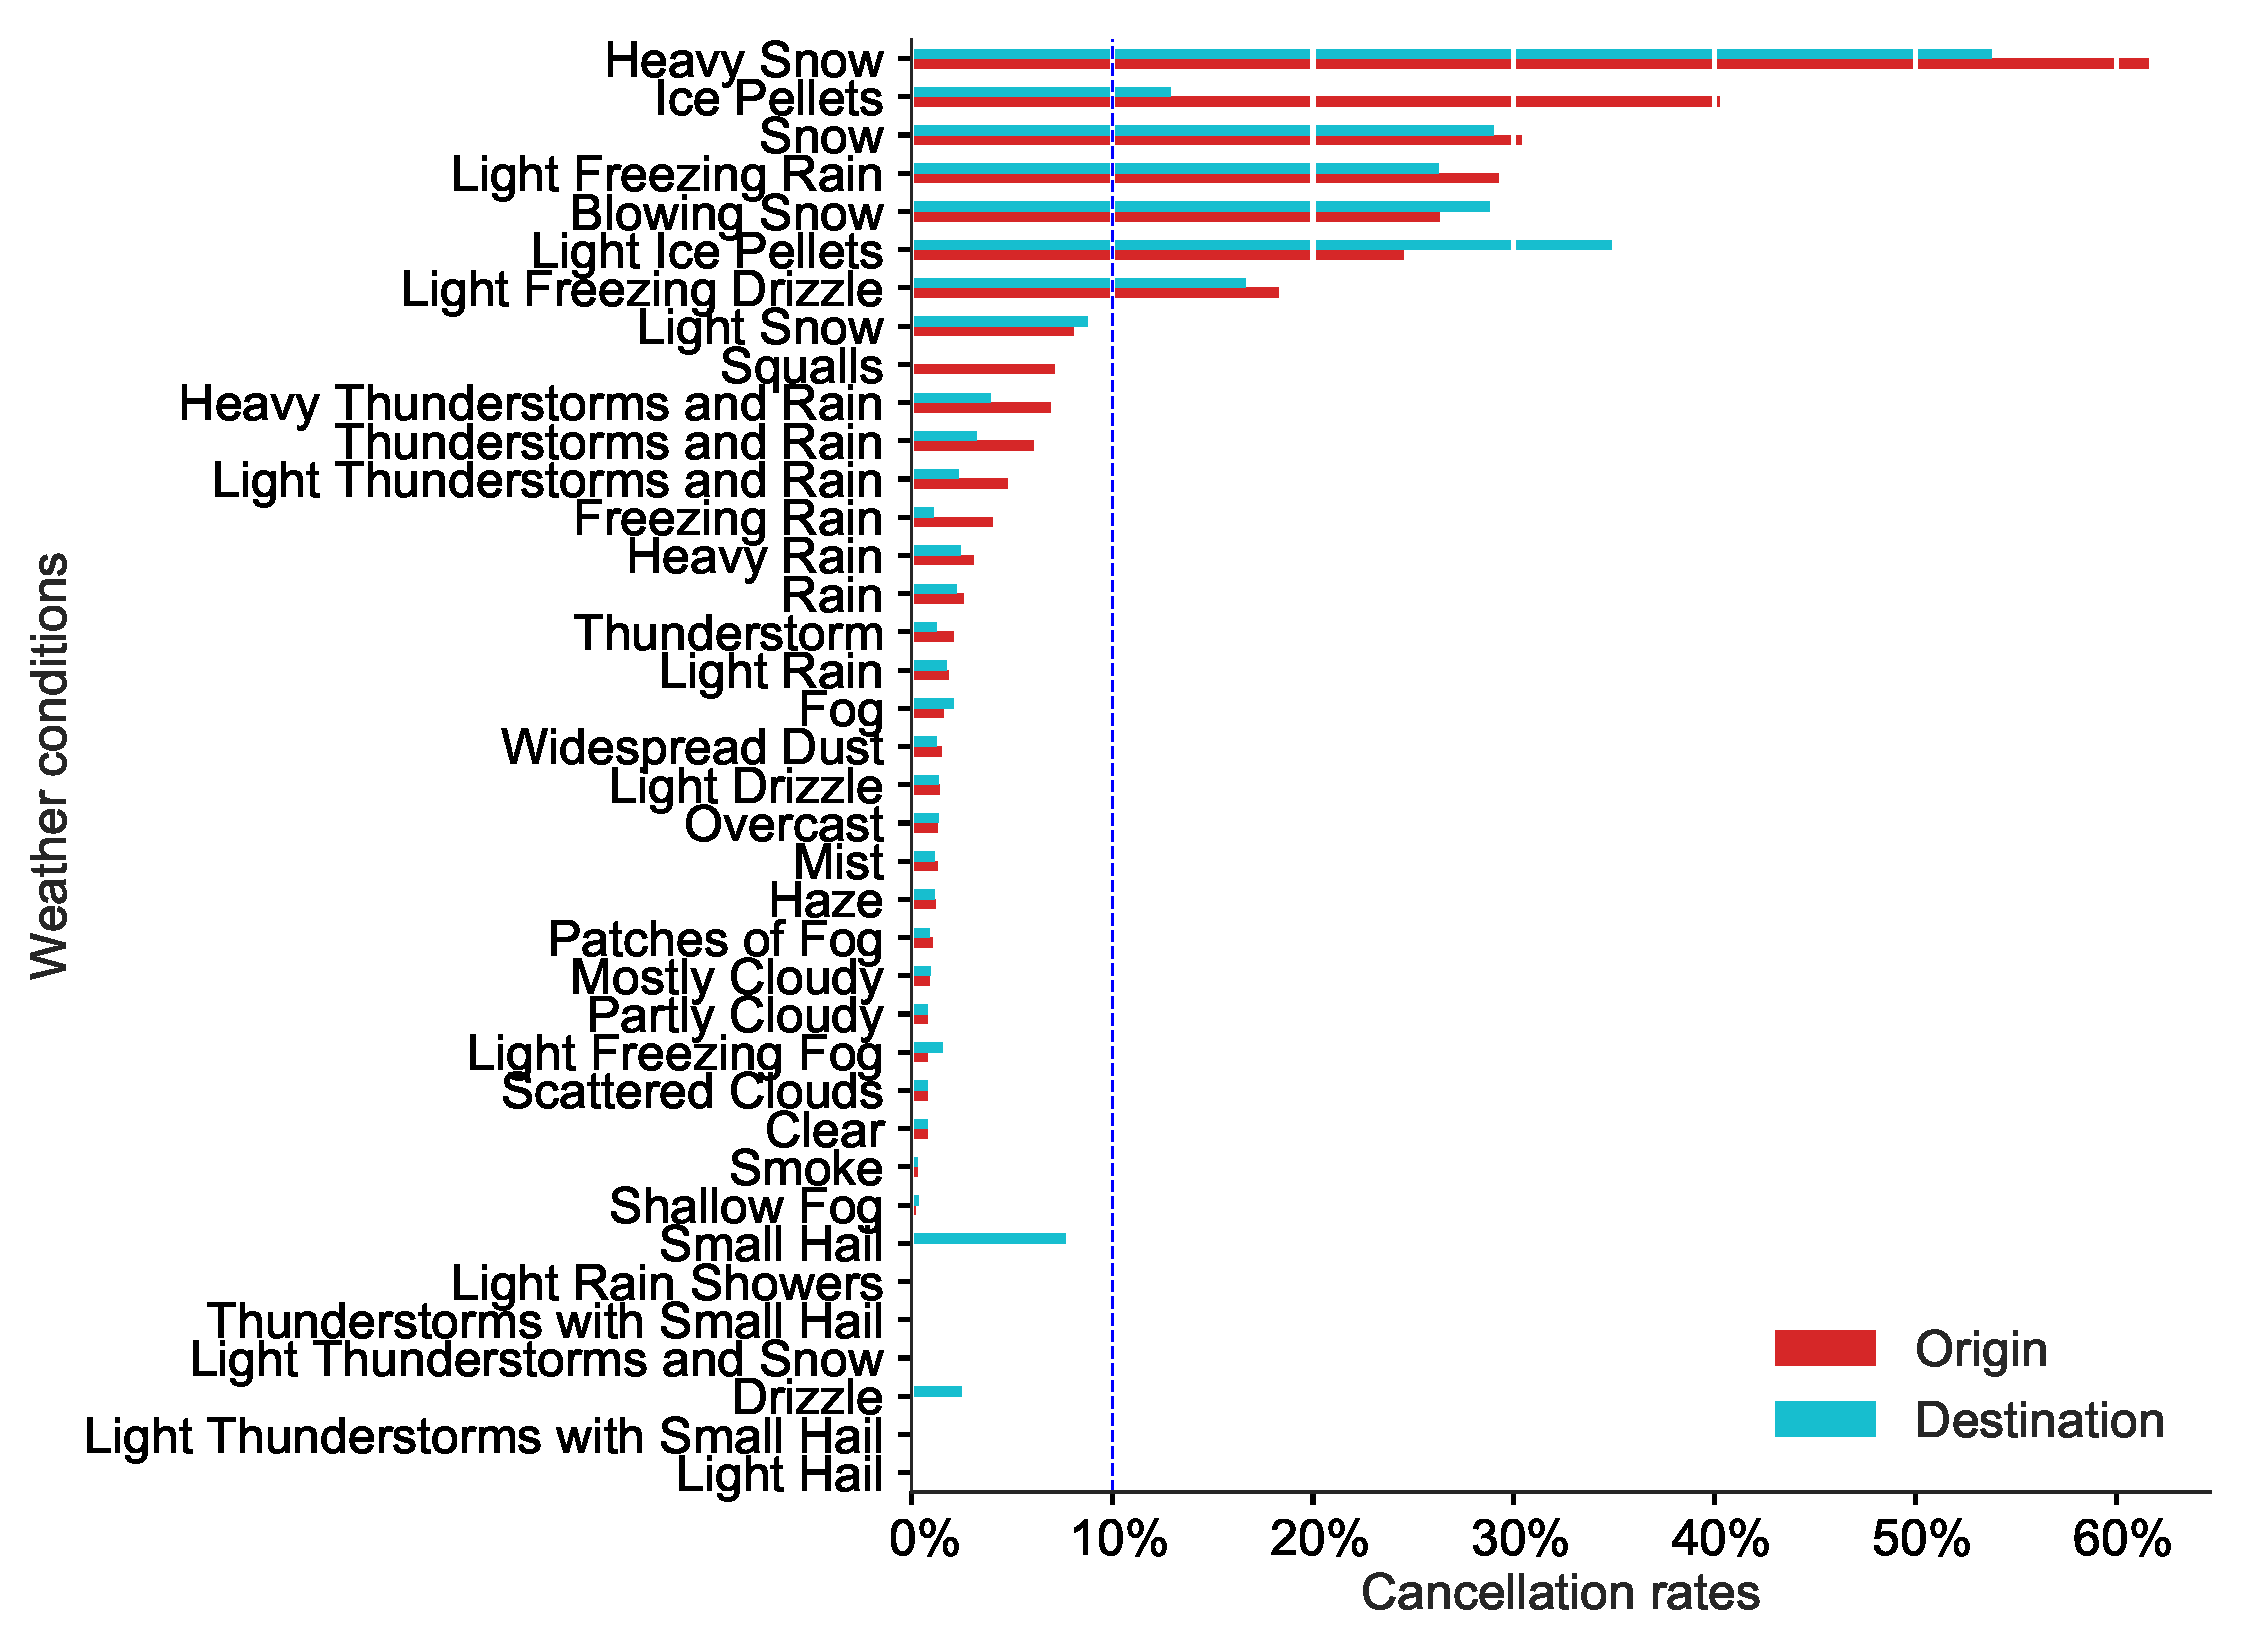
\includegraphics[width=6in]{conditions_canrate.pdf}
\end{center}
\caption{\label{fig:conditionscanrate}
Cancellation rates under different weather conditions at origin and destination airports. The dashed vertical blue line indicates 10$\%$ cancellation rate line.}
\end{figure}
Cancellation rates are pretty high when there are snow related activities at both origin and destination airports. Rain with some thunderstorms also has high cancellation rates. There are similar top weather factors for both locations for cancellation rates greater than 10$\%$ (indicated by blue dashed line), with an exception such as ``Squalls" which has very low cancellation rate at destination and high rates at the origin airports. However, this observation is not significant as there are only 28 records for Squalls at origin. Similarly, the cancellation rates are almost 0 when there are any type of hail conditions. Again, the number of records containing this condition is 69 at origin, so this observation is also not significant.
%%%%%%%%%%%%%%%%%%%%%%%%%
\subsection{Historical Performances}
\label{subsec:historical}
%%%%%%%%%%%%%%%%%%%%%%%%%
For historical performances of a given flight, we have the number of cancellations, number of diversions, departure delays, arrival delays and taxi times for last ``ndays", where we have three values of ndays = 10, 20 and 30. Figure \ref{fig:candivcanrate} shows the influence of the number of cancellations and diversions in the last ndays on the cancellation rate of the flight in question. Each data point in this figure is the result of some calculations. For example, to calculate the cancellation rate for a given number of cancellations ($N_c$), we pick all the flights for which the number of cancellations were $N_c$ in the last ndays. We then count the number of such flights, and also the number of cancelled flights. The ratio then gives us the cancellation rate for $N_c$. We can perform the similar steps for all other historical performance variables but let us first discuss Fig. \ref{fig:candivcanrate}.
\begin{figure}[h!]
\begin{center}
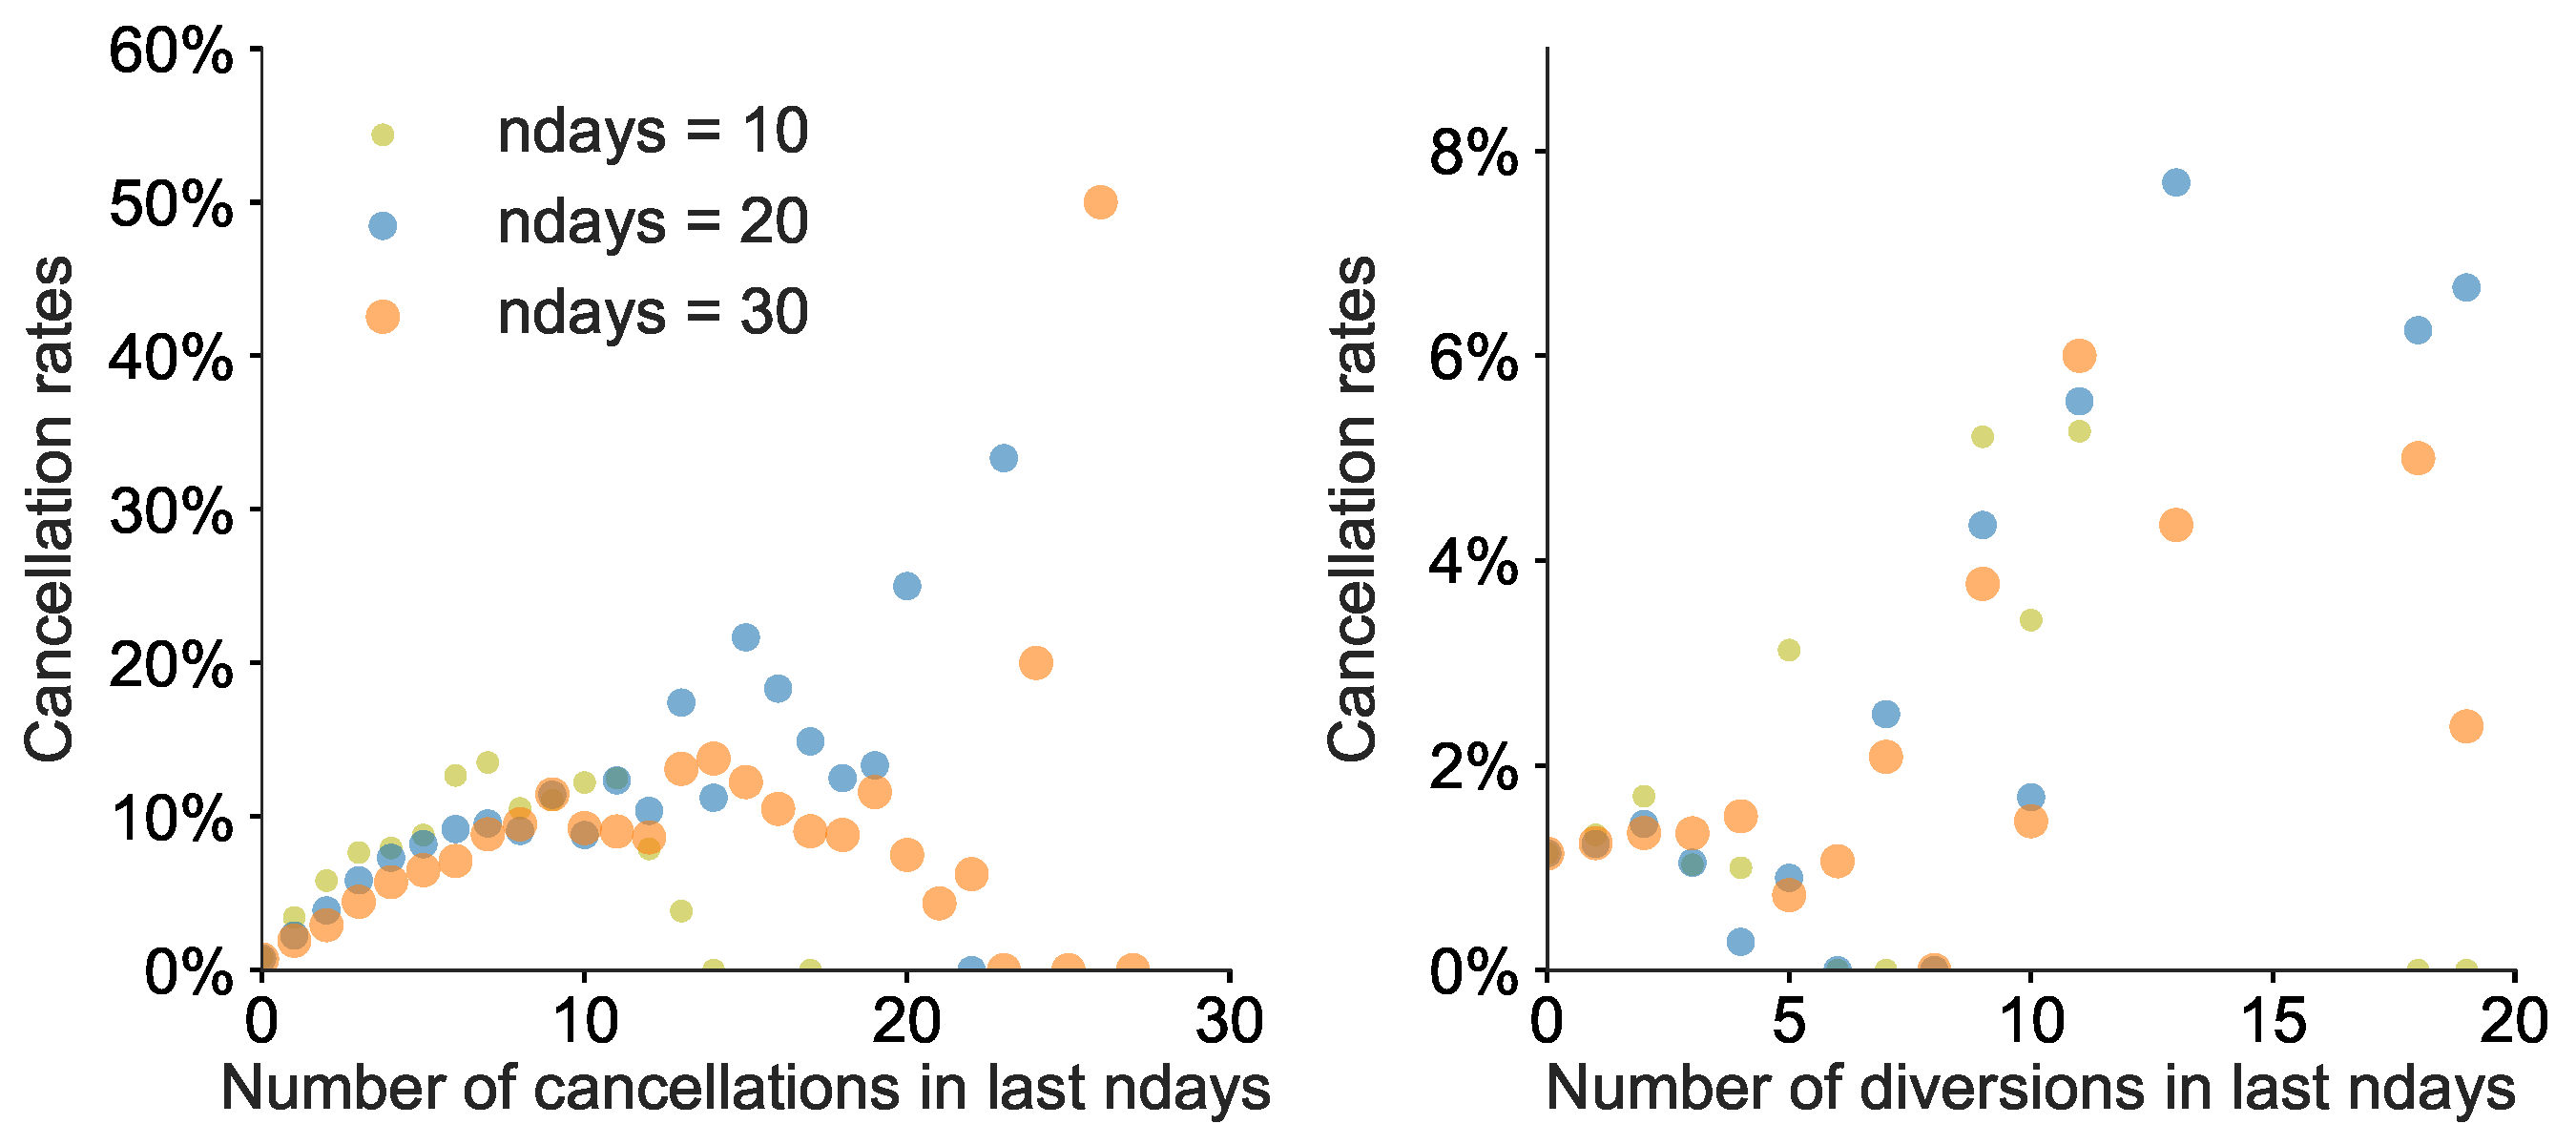
\includegraphics[width=6in]{candiv_canrate.pdf}
\end{center}
\caption{\label{fig:candivcanrate}
Cancellation rates as a function of the number of cancellations and the number of diversions in the last ndays.}
\end{figure}
For the left panel figure, we observe a parabolic pattern with maximum in cancellation rates occurring at different values of the number of cancellations for different values of ndays. There also appears to be some outliers in all three cases, usually at higher values of the number of cancellations in last ndays.
For the right panel figure, generally, the cancellation rates for a flight is higher when the number of diversions of that flight in the last ndays are higher.


Sometimes, we come across a flight for which we do not find any history in the last ndays. We call such flights as temporary flights. The term ``temporary" could be different for different ndays. For example, a flight can be temporary if looked at 10 days history but ``routine" if looked at 30 days history. Figure \ref{fig:historyindicatorcanrate} (a) compares the cancellation rates for temporary (Yes) and routine (No) flights  for all three ndays. Usually, the cancellation rates are higher for temporary flights.  
\begin{figure}[h!]
\begin{center}
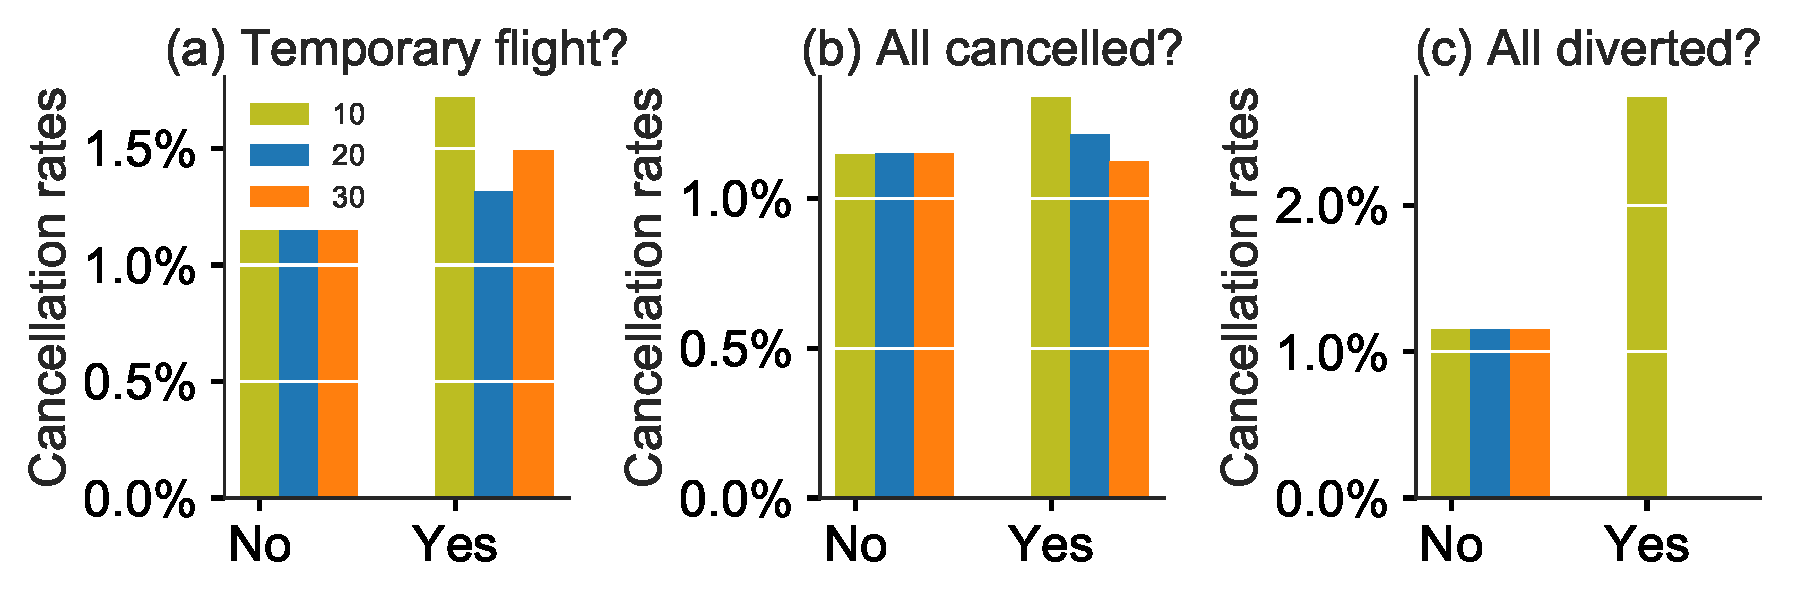
\includegraphics[width=6in]{history_indicator_canrate.pdf}
\end{center}
\caption{\label{fig:historyindicatorcanrate}
Cancellation rate comparisons for three different history indicators, and for all three ndays. The legend 10, 20 and 30 indicates different ndays.}
\end{figure}
There are also some flights for which the history tells that all the flights in last ndays got cancelled. The cancellation rates are slightly higher when all flights got cancelled in the last ndays, as seen in Fig. \ref{fig:historyindicatorcanrate} (b). Similarly, there are flights for which there were 100$\%$ diverted flights in the last ndays. We found such cases only for ndays=10 and the cancellation rates are about 3 times higher as compared to the flights for which the history had no 100$\%$ diversions, as shown in Fig. \ref{fig:historyindicatorcanrate} (c).


Now, we look at the influence of departure delays statistics on cancellation rates. Figure \ref{fig:depdelaymediancanrate} presents the cancellation rates for given median values of the departure delays in the last ndays. 
\begin{figure}[h!]
\begin{center}
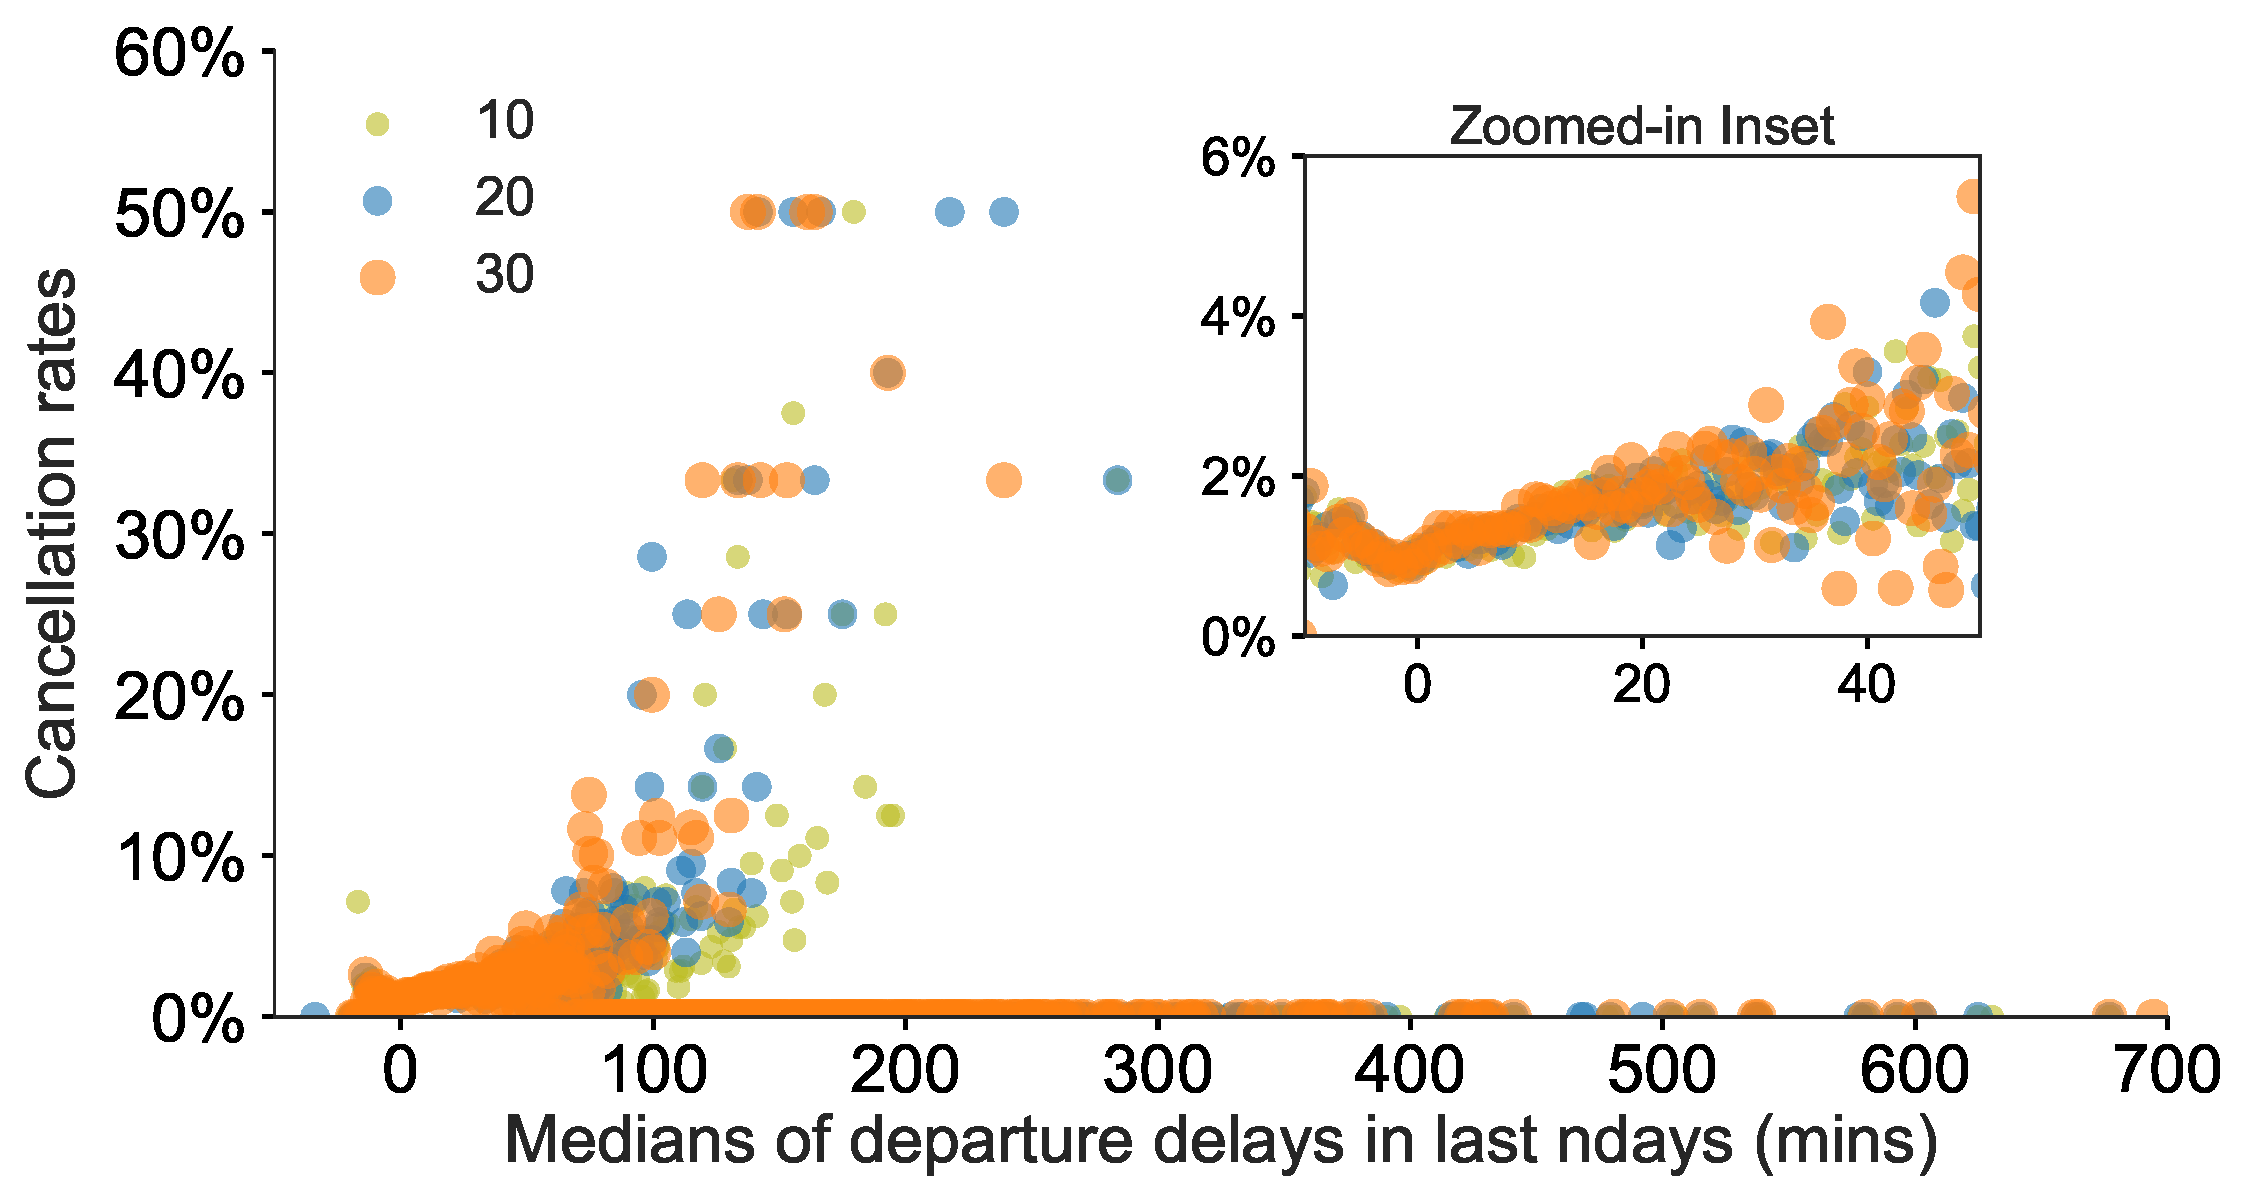
\includegraphics[width=6in]{depdelaymedian_canrate.pdf}
\end{center}
\caption{\label{fig:depdelaymediancanrate}
Cancellation rates as a function of the medians of departure delays in the last ndays. The legend 10, 20 and 30 indicates different ndays. The inset figure has the same x and y labels as the main figure.}
\end{figure}

Cancellation rates are 0 (except a couple of instances) when the medians of departure delays in last ndays days were greater than 200 minutes. For less than 200 mins, and more specifically between 0 and 70 mins, there is a somewhat increasing cancellation rate as a function of median values, as displayed in the inset figure. Statistically significant correlations (Spearman's $\rho$ = 0.77, 0.69, 0.55, for ndays = 10, 20, 30, respectively) are found for all three ndays data in 0-70 mins range.  


In a similar fashion, we can also look at the effect of medians of arrival delays in Fig. \ref{fig:arrdelaymediancanrate}.
\begin{figure}[h!]
\begin{center}
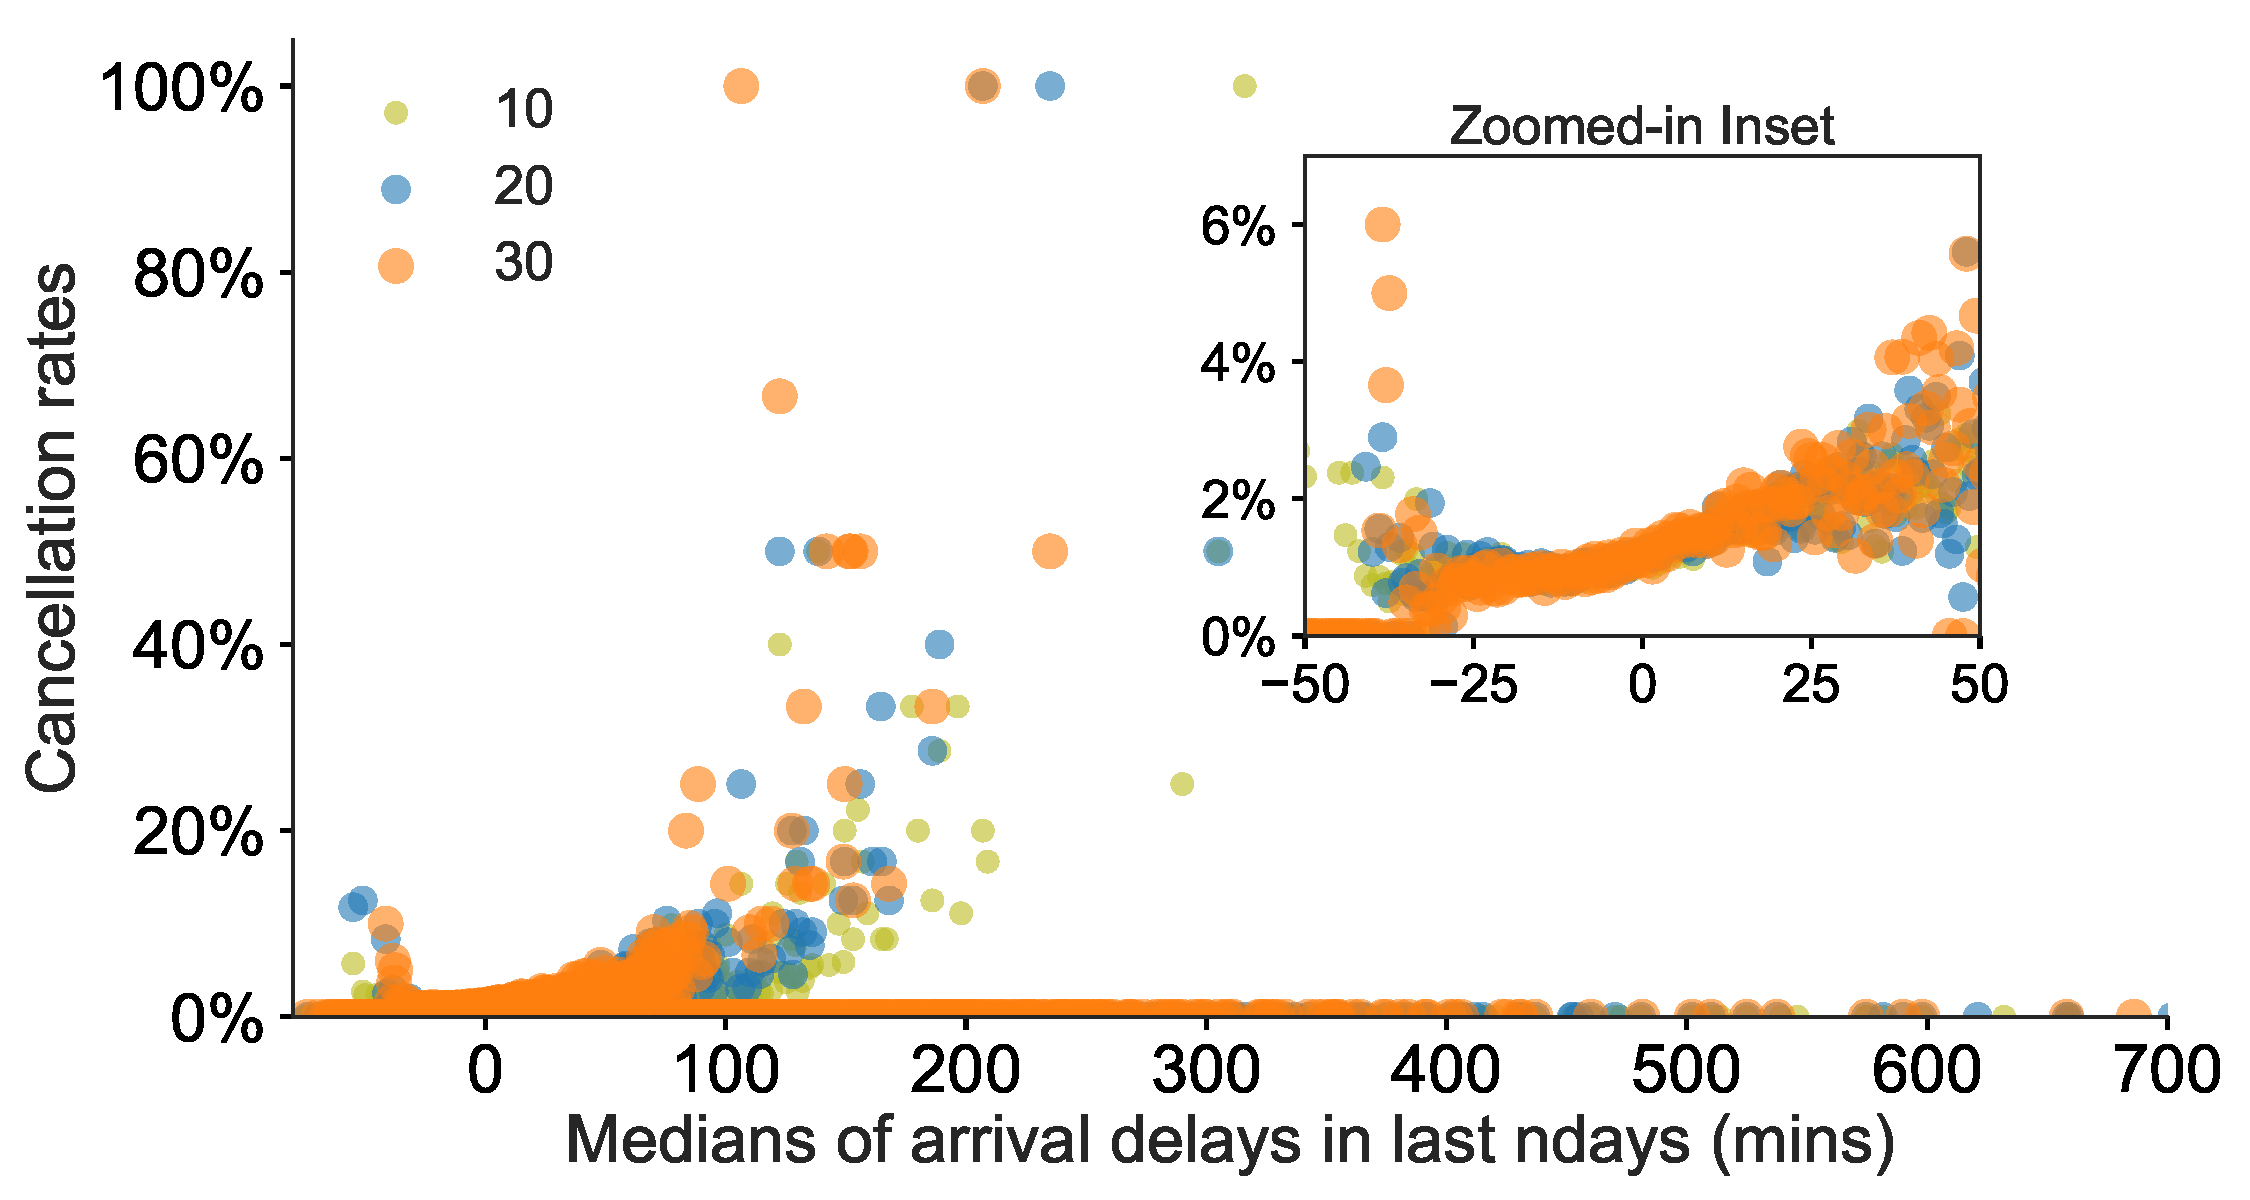
\includegraphics[width=6in]{arrdelaymedian_canrate.pdf}
\end{center}
\caption{\label{fig:arrdelaymediancanrate}
Cancellation rates as a function of the medians of arrival delays in the last ndays. The legend 10, 20 and 30 indicates different ndays. The inset figure has the same x and y labels as the main figure.}
\end{figure}
This scatter plot looks very similar to the one that we got for medians of departure delays. For more than about 200 mins arrival delays, the cancellation rates are 0 for any ndays history. However, when we zoom-in the plot between -50 to 50 mins, we observe a non-monotonic behavior.   
%%%%%%%%%%%%%%%%%%%%%%%%%
\section{Modeling}
\label{sec:models}
%%%%%%%%%%%%%%%%%%%%%%%%%
Knowing the labels for flight cancellations, i.e. 0 for not cancelled and 1 for cancelled, we use supervised machine learning algorithms to build a predictive model. Furthermore, since there are only two outcomes (or classes) in the data (0 and 1), we use binary classification algorithms. The models are trained using the 50$\%$ of the data and the remaining 50$\%$ is used to evaluate the performance of the models. Out of about 2.85 millions flights in 2015-2016, only about 1.15$\%$ flights got cancelled, hence we have a highly imbalanced data. Mostly, all standard algorithms are not well suited for learning with highly imbalanced data. The reason for this difficulty is that the learning in most algorithms is biased towards the majority class. In other words, for highly imbalanced data set, the classification algorithms fail to predict positive class in reasonable numbers. To address this issue, either training data is resampled so that the learning algorithm gets balanced data and learns to predict both classes reasonably well, or the training data is weighted more for minority class and less for majority class. Not only this resampling matters but also the evaluation metric to measure the performance of the model plays a vital role. For example, the accuracy can be really high even if none of the minority class examples are predicted. There are many different types of evaluation metrics that are appropriate for imbalanced classes. Shortly, we will go through some classification algorithms and build predictive models by keeping the imbalanced data challenge issue in our mind. 
%%%%%%%%%%%%%%%%%%%%%%%%%
\subsection{Data Pre-processing}
\label{sec:preproc}
%%%%%%%%%%%%%%%%%%%%%%%%%   
Before feeding the data into any machine learning algorithms, there are some pre-processing steps that must be performed on the data. We outline these steps below. Note that some of the steps are not required (or not good for the best results) in some algorithms, but we list below all the pre-processing steps (in order that they are performed) that we used across all classification algorithms in this work:

\begin{enumerate}  
\item \textbf{Label encoding:} In the dataset, there are some variables with numerical values, some variables with categories and some variables with binary values (0 and 1). For numerical and binary variables, we do not worry about labelling. However, we perform label encoding for the categorical variables. This step is carried out on the whole dataset. 
\item \textbf{Data splitting:} The second step involves splitting the label encoded dataset into train and test datasets. In this project we split them equally with 50$\%$-50$\%$ ratio. Also, we split them in such a manner that the fractions of both classes remain almost same in train and test datasets.
\item \textbf{Resampling or weighting:} In the third step, we take care of the imbalanced data issue by addressing it at the data level by either resampling or weighting the training dataset. Resampling may involve undersampling the majority class examples or oversampling the minority class examples. One can also use the combinations of under and over sampling techniques. There also exists Synthetic Minority Oversampling Technique (SMOTE) which generates synthetic training data for minority class examples by using interpolations. Sometimes, rather than resampling, weighting the training samples works best. In the weighting technique, more weights are given to minority class examples. Different resampling techniques and weighting techniques work best for different algorithms, so we try few different techniques with all the classification algorithms in this project and pick the best ones.  
\item \textbf{Scaling:} For some algorithms, it is necessary that we scale the values of all features to lie within a fixed range. We scale features such that all features have values between 0 and 1. 
\end{enumerate}

After scaling the features, we can also reduce the feature space by selecting features that have most predictive power. Different techniques such that $\chi^2$ test or even principal component analysis (PCA) can be used to do so. However, in this project we have not performed any feature selection at this stage. 
%%%%%%%%%%%%%%%%%%%%%%%%%
\subsection{Modeling Pipeline and Evaluation Metric}
\label{sec:pipe}
%%%%%%%%%%%%%%%%%%%%%%%%%   
Once the data is pre-processed, we feed them to classification algorithm to build the model. In order to evaluate the performance of the model, we test the model on the test data set. Before making predictions on test dataset, we use the exact same pre-processing steps that we used for training dataset and apply them on the test dataset. Python's scikit learn library has a very useful class called ``pipeline" which we use to combine all the steps, i.e. pre-processing and classifier learning steps into one. This pipeline is then applied directly on the test dataset. Let us now go through each models that we used in this project. Note that for some algorithms, training the 50$\%$ of the data, which is about 1.4 million examples, is very slow. For such algorithms, we first consider only the 10$\%$ of the whole data. We then follow the pre-processing steps on the 10$\%$ of the data. Once we know the optimal hyperparameters  and the best resampling/weighting technique, we then use the whole data to build the model. For tuning hyper-parameters we use 5-fold cross validation with grid search method in sklearn. We run the cross validation to obtain the optimal hyperparameters for all considered resampling/weighting techniques. 


One more important consideration while performing cross validation is the selection of a proper evaluation metric. Especially, for imbalanced data, it is important to be careful about the choice of the evaluation metric. Our aim is to predict the flight cancellation likelihood with data containing only about 1.14$\%$ of the cancelled flights in 2015-2016. Accuracy is not a good metric for such datasets. We definitely want to have high true positive rate (or recall) with cancelled flight tagged as positive class. At the same time, we do not want lots of false positives or less precision. Most of the time, the choice of a good metric depends on business needs. In this project, we keep in mind all elements of a confusion matrix. Also, we want a metric which is threshold invariant, so F1-score is also not a great choice. There are two popular metrics such as area under the curve (AUC) of receiver operating characteristic (ROC) curve and AUC of precision recall (OR) curve. \href{http://ftp.cs.wisc.edu/machine-learning/shavlik-group/davis.icml06.pdf}{Theoretically}, ROC curves are useful in an algorithm that optimizes PR AUC. Also, \href{http://journals.plos.org/plosone/article?id=10.1371/journal.pone.0118432}{T. Saito and M. Rehmsmeier} found that for imbalanced data, precision recall curve is more informative than ROC curve.


So, we will stick with PR AUC as our scoring parameter for tuning hyperparameters.
%%%%%%%%%%%%%%%%%%%%%%%%%
\subsection{Logistic Regression}
\label{sec:LR}
%%%%%%%%%%%%%%%%%%%%%%%%%  
For logistic regression algorithm, we use all 4 pre-processing steps mentioned in Sec. \ref{sec:preproc}. Training is pretty slow for the 50$\%$ of the whole data, so we consider only the 10$\%$ of the whole data to tune hyperparameters and find best resampling/weighting technique. Table \ref{tab:LR} shows the results for various metrics for all different resampling/weighting techniques that we tried. 
\begin{table}[!h]
\centering
\caption{Logistic regression classifier - choosing the best resampling/weighting technique }\label{tab:LR}
\scalebox{0.75}{
\begin{tabular}{lllcccccc}
\toprule
\textbf{Resampling/weighting technique} & \textbf{Class}  & \multicolumn{3}{c}{\textbf{Values}} & \textbf{PR AUC} & \textbf{ROC AUC} & \textbf{CPU time (min)} \\
\cmidrule{3-5}
 & & Precision & Recall & F1-score \\
\midrule
RandomUnderSampler (10$\%$) & 0 & 0.99 & 1.00 & 0.99 & 0.51 & 0.50 & 0.01 \\ [-1.3ex]
\addlinespace
    & 1 & 0.00 & 0.00 & 0.00 \\
\hline
SMOTE (10$\%$) & 0 & 0.99 & 1.00 & 0.99 & 0.51 & 0.50 & 0.1 \\ [-1.3ex]
\addlinespace
    & 1 & 0.00 & 0.00 & 0.00 \\
\hline
No resampling, using weighting (10$\%$) & 0 & 0.99 & 1.00 & 0.99 & 0.51 & 0.50 & 0.03  \\ [-1.3ex] 
\addlinespace
    & 1 & 0.00 & 0.00 & 0.00 \\
\hline
\gc Final - RandomUnderSampler (100$\%$) & \gc 0 & \gc 0.99 & \gc 1.00 & \gc 0.99 & \gc 0.51 & \gc 0.50 & \gc 0.1  \\ [-1.3ex]
\addlinespace
\gc    & \gc 1 & \gc 0.00 & \gc 0.00 & \gc 0.00 & \gc & \gc & \gc \\
\bottomrule \\
\end{tabular}
}
\end{table}
We found, using 10$\%$ of the whole data, that all techniques led to very poor model. However, the random under sampling technique (RandomUnderSampler in sklearn) spent least computational time. So, we used random undersampling technique and build the classifier using the whole data (1.4+ million examples in training dataset). This model is represented as final model and colored in green in Tab. \ref{tab:LR}, and the ROC and PR curves are shown in Fig. \ref{fig:LR} . 
\begin{figure}[!h]
\begin{center}
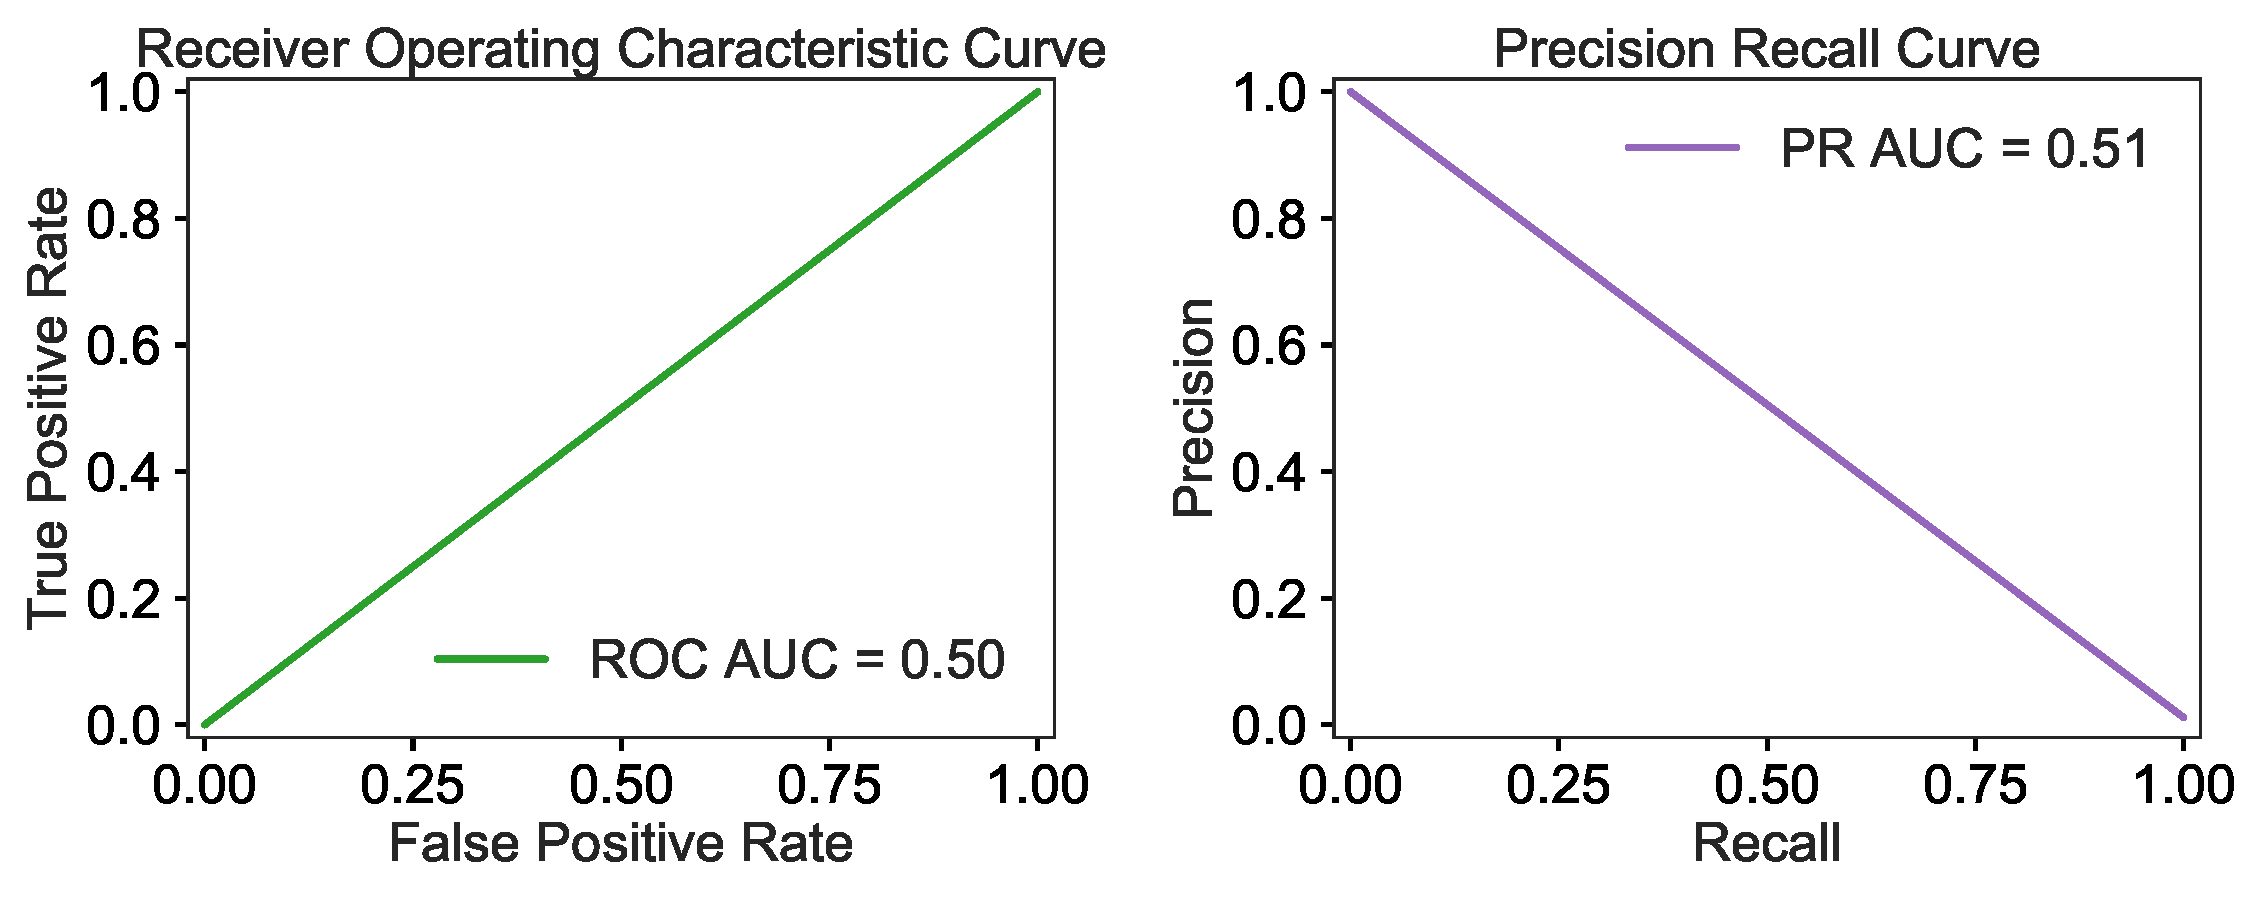
\includegraphics[width=6in]{LR_ROC_PR_plots.pdf}
\end{center}
\caption{\label{fig:LR}
ROC and PR curves for the logistic regression classifier.}
\end{figure}
Testing on the holdout data (50$\%$ of the whole data) gave us the same poor results. In conclusion, by maximizing PR AUC, the logistic regression algorithm produces predictions that are absolutely by "chance" or "luck" by penalizing the coefficients very strongly (very high regularization). This also means that we get high bias model, i.e. under-fit model, which explains the term "luck". Also, the model does not predict even a single flight cancellation, which leads to zero recall, precision and hence F1-score. In other words, the model works really well but only for negative class, i.e. non-cancelled flights. Upon trying a different metric (such as F1-score or recall) for optimization in cross validation step, we obtained non-zero values for precision, recall and F1-score but the PR AUC was too low. Again, choosing a metric depends on business requirements. In this project, we fix the scoring parameter to be PR AUC across all classifiers, so we accept the poor results that we get from logistic regression.
%%%%%%%%%%%%%%%%%%%%%%%%%
\subsection{Gaussian Naive Bayes}
\label{sec:NB}
%%%%%%%%%%%%%%%%%%%%%%%%%   
We use Gaussian Naive Bayes classifier and the first three steps of the pre-processing steps mentioned in Sec. \ref{sec:preproc}. This algorithm is not that slow so we use the whole dataset and split that into train and test (holdout) datasets with 50$\%$-50$\%$ ratio. Table \ref{tab:GNB} shows the results for various metrics for all different resampling techniques that we tried. Note that the Naive Bayes classification implementation in sklearn does not have any option for weighting the classes. So, here we try only two resampling techniques. 
\begin{table}[!h]
\centering
\caption{Gaussian Naive Bayes classifier - choosing the best resampling technique }\label{tab:GNB}
\scalebox{0.75}{
\begin{tabular}{lllcccccc}
\toprule
\textbf{Resampling/weighting technique} & \textbf{Class}  & \multicolumn{3}{c}{\textbf{Values}} & \textbf{PR AUC} & \textbf{ROC AUC} & \textbf{CPU time (min)} \\
\cmidrule{3-5}
 & & Precision & Recall & F1-score \\
\midrule
\gc RandomUnderSampler & \gc 0 & \gc 0.99 & \gc 0.87 & \gc 0.93 & \gc 0.08 & \gc 0.76 & \gc 0.03 \\ [-1.3ex]
\addlinespace
\gc    & \gc 1 & \gc 0.04 & \gc 0.48 & \gc 0.08 & \gc & \gc & \gc \\
\hline
SMOTE & 0 & 0.99 & 0.86 & 0.92 & 0.08 & 0.75 & 1 \\ [-1.3ex]
\addlinespace
    & 1 & 0.04 & 0.53 & 0.08 \\
\bottomrule \\
\end{tabular}
}
\end{table}
Both resampling techniques give PR AUC to be 0.08, which is very poor. However, the random under sampling is faster and also the ROC AUC is slightly better than that obtained using SMOTE. So, we choose random under sampling. The chosen model is highlighted in green in Tab. \ref{tab:GNB}. Any Naive Bayes algorithm assumes that the features are independent for a given class. One of the reasons for a very poor PR AUC is probably due to violating this assumption. Therefore, we can try to look at correlations amongst features and remove the ones that are highly correlated. We found many pairs of features that have correlation coefficient values closer to 1. We removed the top 10 features with high correlations and trained the model using the best chosen resampling technique. Removing features did not help in improving the results but also it did not decrease the PR AUC. Finally, we consider the reduced feature set and the resulting ROC and PR curves (obtained by running model on 50$\%$ holdout dataset) are shown in Fig. \ref{fig:GNB}.
 \begin{figure}[!h]
\begin{center}
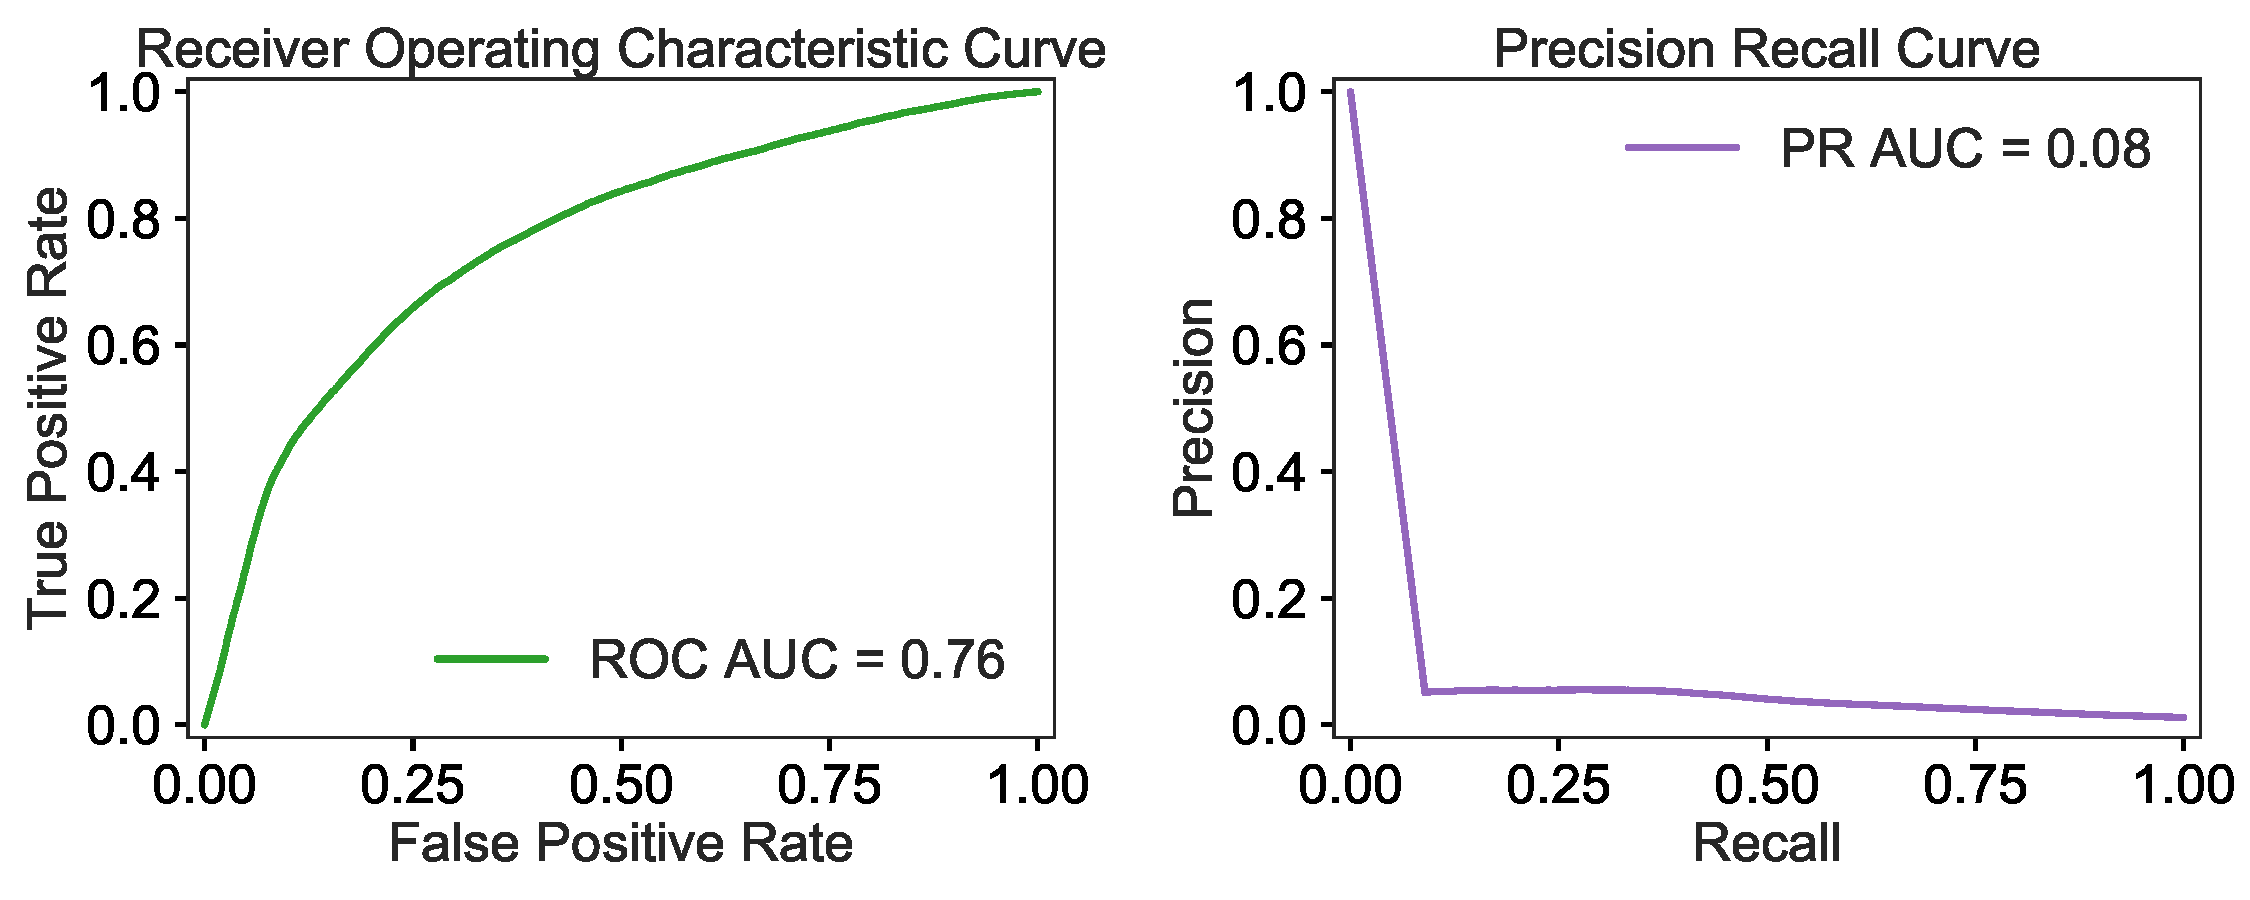
\includegraphics[width=6in]{GNB_ROC_PR_plots.pdf}
\end{center}
\caption{\label{fig:GNB}
ROC and PR curves for the Gaussian Naive Bayes classifier.}
\end{figure}
As far as ROC curves are concerned, Gaussian Naive Bayes is better than logistic regression. The reason PR AUC is so much smaller than ROC AUC is because the ROC curve has information about true negatives which dominate the confusion matrix in the current problem, especially in the bottom left of ROC curve or for very high values of thresholds. We will discuss more about the thresholds and optimum operating point when we compare various models.  
%%%%%%%%%%%%%%%%%%%%%%%%%
\subsection{Random Forest}
\label{sec:RF}
%%%%%%%%%%%%%%%%%%%%%%%%%   
For the random forest model, we do not have to scale the features and so we skip the fourth step in the pre-processing steps mentioned in Sec. \ref{sec:preproc}. This algorithm is also not that slow so we use the whole dataset and split that into train and test (holdout) datasets with 50$\%$-50$\%$ ratio. Table \ref{tab:RF} shows the results for various metrics for all different resampling/weighting techniques that we tried.
\begin{table}[!h]
\centering
\caption{Random forest classifier - choosing the best resampling/weighting technique }\label{tab:RF}
\scalebox{0.75}{
\begin{tabular}{lllcccccc}
\toprule
\textbf{Resampling/weighting technique} & \textbf{Class}  & \multicolumn{3}{c}{\textbf{Values}} & \textbf{PR AUC} & \textbf{ROC AUC} & \textbf{CPU time (min)} \\
\cmidrule{3-5}
 & & Precision & Recall & F1-score \\
\midrule
RandomUnderSampler & 0 & 1.00 & 0.81 & 0.90 & 0.24 & 0.85 & 0.17 \\ [-1.3ex]
\addlinespace
    & 1 & 0.04 & 0.73 & 0.08 \\
\hline
SMOTE & 0 & 0.99 & 1.00 & 0.99 & 0.28 & 0.82 & 30 \\ [-1.3ex]
\addlinespace
    & 1 & 0.70 & 0.15 & 0.25 \\
\hline
\gc No resampling, using weighting & \gc 0 & \gc 0.99 & \gc 1.00 & \gc 0.99 & \gc 0.33 & \gc 0.84 & \gc 10  \\ [-1.3ex] 
\addlinespace
\gc    & \gc 1 & \gc 0.67 & \gc 0.21 & \gc 0.32 & \gc & \gc & \gc \\
\bottomrule \\
\end{tabular}
}
\end{table}
The random forest model has many hyperparameters to be optimized. Using 5-fold cross validation, we optimized all hyperparameters except the number of trees. For Tab. \ref{tab:RF}, we used 50 trees.  In order to improve further, we can increase the number of trees in the random forest. However, the computational cost will go up by doing so. We can play with the trade-off and pick the number of trees such that beyond that number the PR AUC does not increase much. Figure \ref{fig:RF_trees} shows that the PR AUC improves by increasing the number of trees but at the cost of computational time.
\begin{figure}[!h]
\begin{center}
\includegraphics[width=4in]{RF_tree_effects.pdf}
\end{center}
\caption{\label{fig:RF_trees}
PR AUC (green) and CPU time (red) as a function of the number of trees. The vertical blue line indicates 50 trees.}
\end{figure}
The PR AUC  seems to be leveling off asymptotically after around 40-50 trees. In other words, for more than 50 trees, the gain in PR AUC is not as significant as the increase in computational cost is. So, we stick with 50 trees. With 50 trees, and all other optimized hyper-parameters, we can now try to play with feature selections which is one of a by products of the random forest model. 
\begin{figure}[!h]
\begin{center}
\includegraphics[width=6in]{RF_FI.pdf}
\end{center}
\caption{\label{fig:RF_FI}
Top 20 features (out of 67) as given by feature importance from the random forest model. Most important features are at the bottom. The horizontal line indicates standard deviation on feature importance.}
\end{figure}
Figure \ref{fig:RF_FI} shows the top 20 features in terms of their feature importances. Out of these top 20 features, 10 have information about the weather, 4 are historical performance features (which we engineered), 4 are calendar variables and remaining two have information about the flight (Carrier and Distance). The calendar variables do not make much sense here because it is quite possible that Month and Month\_Dest have quite the same information. Similarly, DayofMonth and DayOfMonth\_Dest are very much the same in terms of information. Moreover, there are other calendar variables such as DayOfWeek which seemed a better predictor than DayOfMonth in Sec. \ref{subsec:calvar}. In order to find optimal choice of features that maximize PR AUC, we use different values of cutoffs on feature importance and obtain PR AUC. Figure \ref{fig:RF_FI_Cutoff} informs us that the PR AUC is almost constant when the cutoff is less than 0.02. However, there seems like a maximum when we remove features whose feature importance values are less than 0.009. 
\begin{figure}[!h]
\begin{center}
\includegraphics[width=4in]{RF_FI_Cutoff.pdf}
\end{center}
\caption{\label{fig:RF_FI_Cutoff}
PR AUC as a function of feature importance cutoff.}
\end{figure}
We can use the reduced set of features (using cutoff of 0.009) and train the model again. However, before that, there is one more item that we have not yet tried, and that is one hot encoding. We should have done it in the beginning but luckily there is no problem because all the features that we are going to remove are either binary or numerical. In one-hot encoding (OHE) we need to worry about only categorical variables. After doing OHE, we create additional features containing 0s and 1s. We find that performing OHE does not help in improving PR AUC. Therefore, there is no advantage of doing OHE. It in fact slows down the computation due to increased number of features (dummy ones). So, finally we only use the reduced set of features (with feature importance greater than 0.009), with weighting training data (no resampling), and use 50 trees, and re-train the model. The PR AUC on the test dataset is found to be 0.33, which is same as what we found with all features. Since we get the same results with less number of features, we stick with less number of features. Figure \ref{fig:RF} displays the ROC and PR curves based on the test dataset.
 \begin{figure}[!h]
\begin{center}
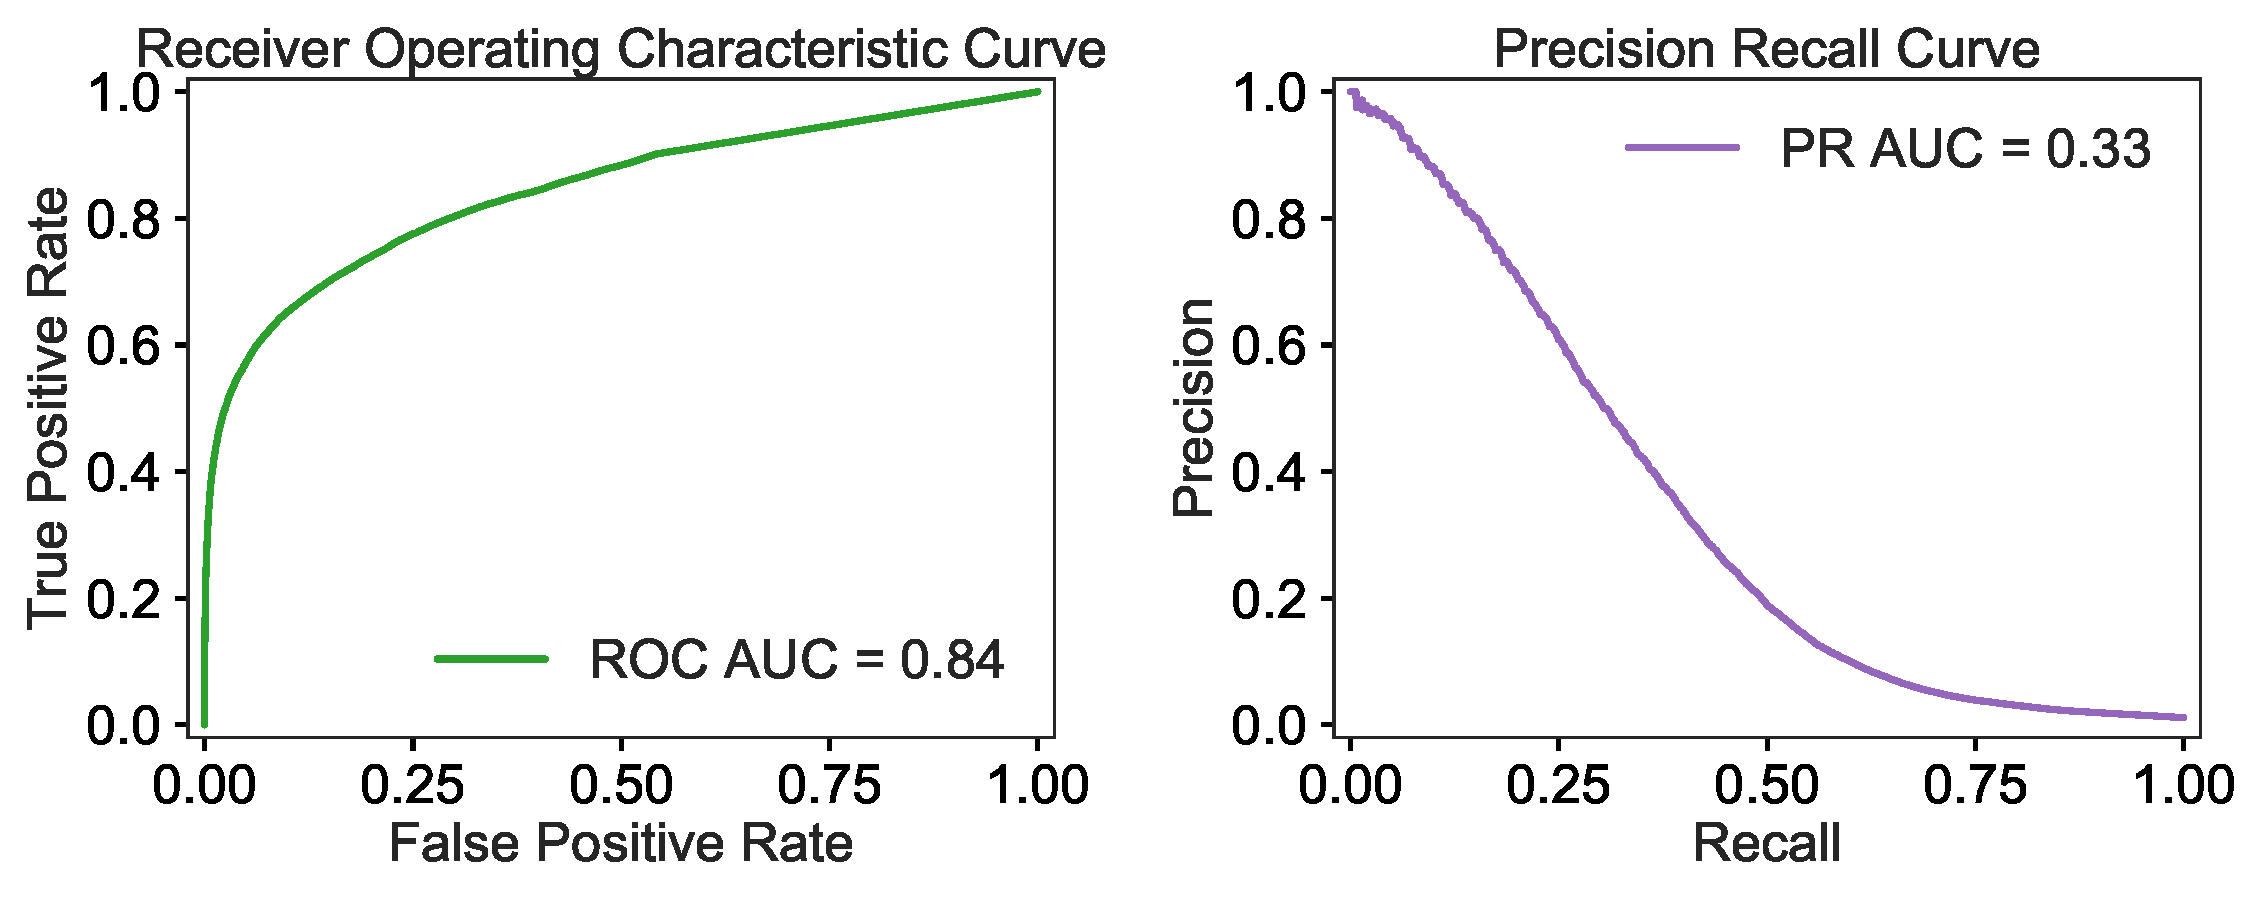
\includegraphics[width=6in]{RF_ROC_PR_plots.pdf}
\end{center}
\caption{\label{fig:RF}
ROC and PR curves for the random forest classifier.}
\end{figure}
The random forest classifier gives us the best model so far. We now go through some more ensemble based approaches to see if we get any improvements.
%%%%%%%%%%%%%%%%%%%%%%%%%
\subsection{Gradient Boosting}
\label{sec:GBC}
%%%%%%%%%%%%%%%%%%%%%%%%%   
For this algorithm also, we do not need to use any feature scaling. However, due to high computational cost we first work with 10$\%$ of the data to find optimum hyperparameters and best resampling/weighting technique. Table \ref{tab:GBC} shows the results for various metrics for all different resampling/weighting techniques that we tried.
\begin{table}[!h]
\centering
\caption{Gradient boosting classifier - choosing the best resampling/weighting technique }\label{tab:GBC}
\scalebox{0.75}{
\begin{tabular}{lllcccccc}
\toprule
\textbf{Resampling/weighting technique} & \textbf{Class}  & \multicolumn{3}{c}{\textbf{Values}} & \textbf{PR AUC} & \textbf{ROC AUC} & \textbf{CPU time (min)} \\
\cmidrule{3-5}
 & & Precision & Recall & F1-score \\
\midrule
RandomUnderSampler & 0 & 1.00 & 0.77 & 0.87 & 0.14 & 0.83 & 0.01 \\ [-1.3ex]
\addlinespace
    & 1 & 0.04 & 0.73 & 0.07 \\
\hline
\gc SMOTE & \gc 0 & \gc 0.99 & \gc 1.00 & \gc 0.99 & \gc 0.18 & \gc 0.80 & \gc 3 \\ [-1.3ex]
\addlinespace
\gc    & \gc 1 & \gc 0.64 & \gc 0.09 & \gc 0.15 & \gc & \gc & \gc \\
\bottomrule \\
\end{tabular}
}
\end{table}
For gradient boosting, we find the SMOTE to be the best resampling technique. The value of PR AUC is not as good as we got for from the random forest model. However, this low value is based on training the model using only 10$\%$ of the data. Before considering the whole data for training, we look at the effect of the number of estimators on PR AUC using the subset of the data. We also study the feature importance, similar to random forest, to select top features. Once we have the optimum model using the subset of the data, we will then use the whole data to train the classifier. We first study the effect of the number of estimators in Fig. \ref{fig:GBC_trees}. 
\begin{figure}[!h]
\begin{center}
\includegraphics[width=4in]{GBC_tree_effects.pdf}
\end{center}
\caption{\label{fig:GBC_trees}
PR AUC (green) and CPU time (red) as a function of the number of estimators. The vertical blue line indicates 60 estimators.}
\end{figure}
Clearly, the PR AUC improves by increasing the number of estimators and it seems to be leveling off at around 60 estimators. So, we will choose 60 estimators for the gradient boosting algorithm. Note that, unlike random forest, the CPU time levels off for more than 50 estimators. With 60 estimators, and all other optimized hyper-parameters, we can now study the feature importance. 
\begin{figure}[!h]
\begin{center}
\includegraphics[width=6in]{GBC_FI.pdf}
\end{center}
\caption{\label{fig:GBC_FI}
Top 20 features (out of 67) as given by feature importance from the gradient boosting model. Most important features are at the bottom.}
\end{figure}
Figure \ref{fig:GBC_FI} shows the top 20 features in terms of their feature importances. Out of these top 20 features, 9 have information about the weather, 3 are historical performance features (which we engineered), 4 are calendar variables and remaining four have information about the flight (Carrier, Distance, Origin and Destination). The calendar variables do not make much sense here because it is quite possible that DayOfWeek and DayOfWeek\_Dest have quite the same information. Similarly, Month and Month\_Dest are very much the same in terms of information. In order to find optimal choice of features that maximize PR AUC, we use different values of cutoffs on feature importance and obtain PR AUC. Figure \ref{fig:GBC_FI_Cutoff} suggests that the PR AUC is maximum when we remove features whose feature importance values are less than 0.015.
\begin{figure}[!h]
\begin{center}
\includegraphics[width=4in]{GBC_FI_Cutoff.pdf}
\end{center}
\caption{\label{fig:GBC_FI_Cutoff}
PR AUC as a function of feature importance cutoff.}
\end{figure}
The gradient boosting classification algorithm is computationally very expensive, so we did not try OHE here. Therefore, as a final case for the gradient boosting model, we use selected features whose feature importances are greater than 0.015, and use SMOTE for oversampling, and use 60 estimators. We now use the whole dataset and the resultant model gives PR AUC to be 0.35 based on the holdout dataset. Figure \ref{fig:GBC} shows the ROC and PR curves based on the test (holdout) dataset.
 \begin{figure}[!h]
\begin{center}
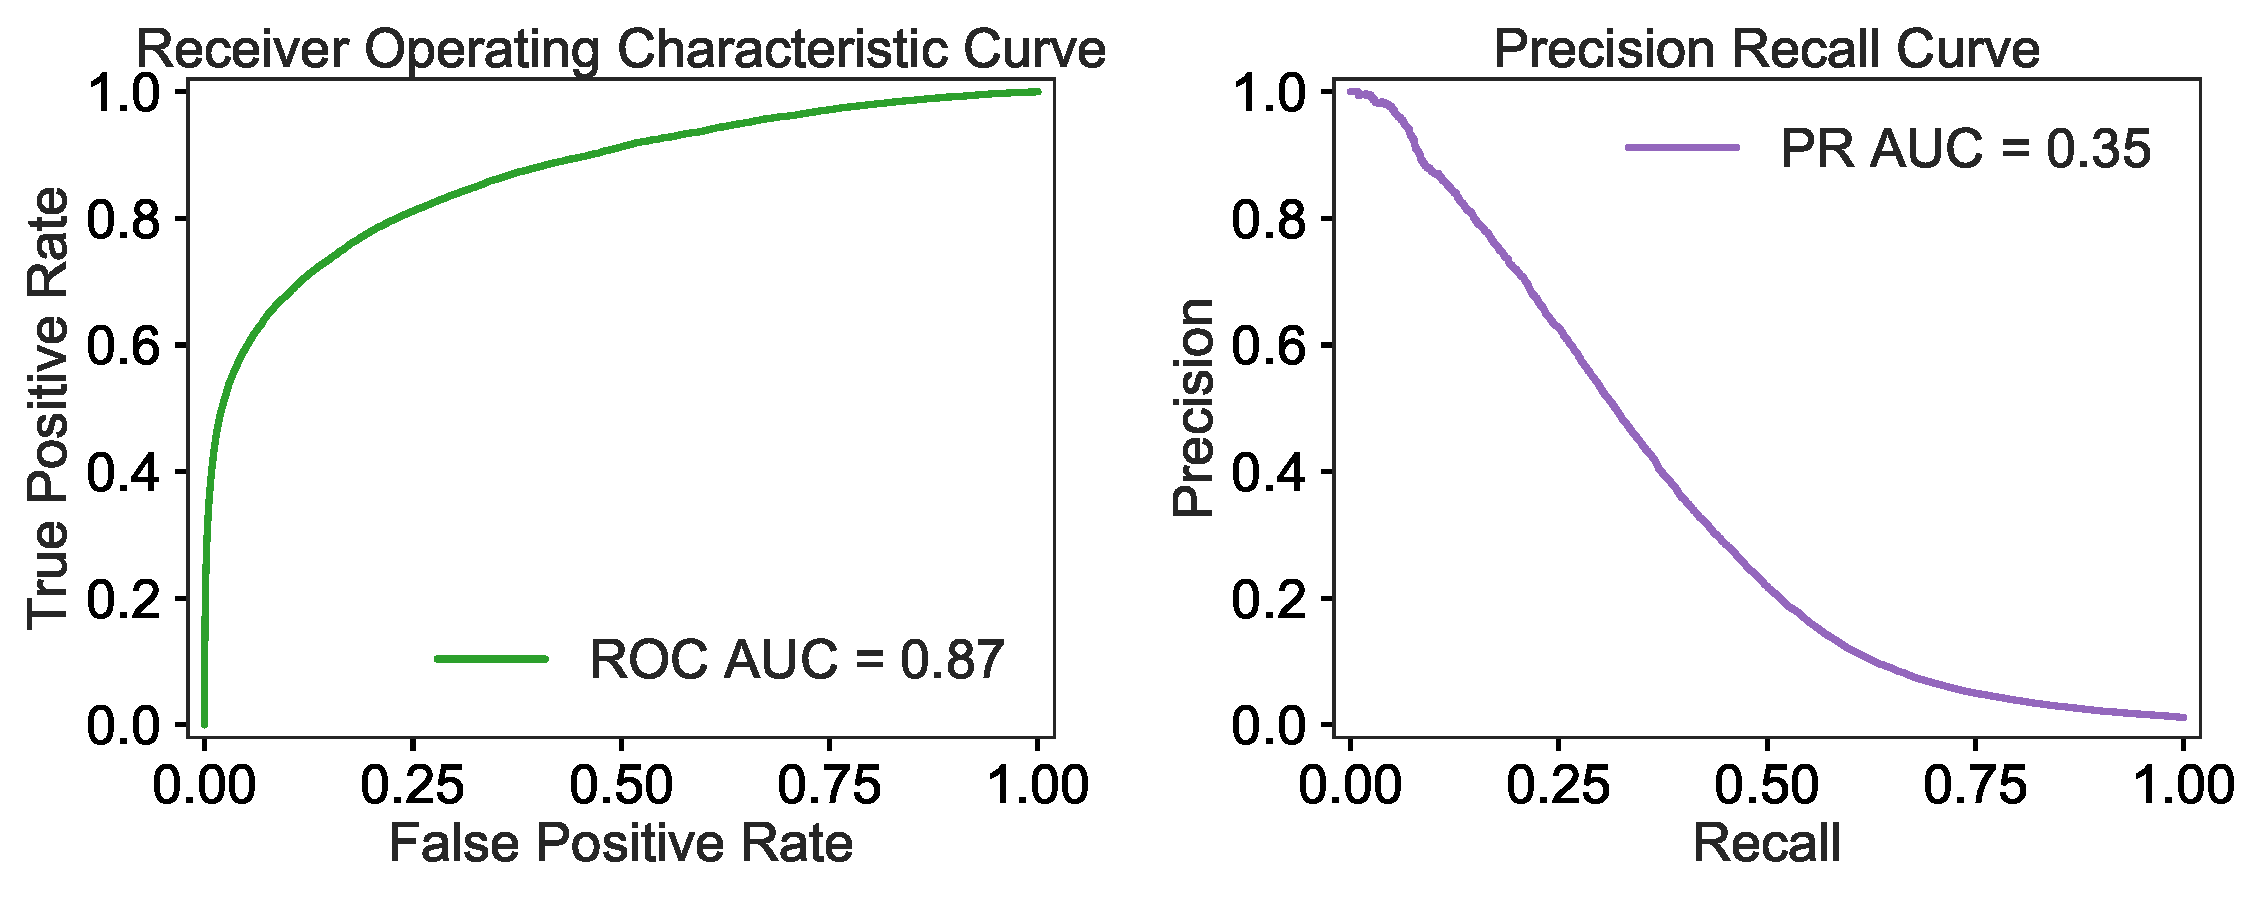
\includegraphics[width=6in]{GBC_ROC_PR_plots.pdf}
\end{center}
\caption{\label{fig:GBC}
ROC and PR curves for the gradient boosting classifier.}
\end{figure}
The gradient boosting gives us PR AUC better than that obtained through random forest, but with cost of significant CPU time. It took about 27 hours to train the gradient boosting classifier using the 50$\%$ of the whole dataset on an i-Mac with 4 GHz Intel Core i7 processor. 
%%%%%%%%%%%%%%%%%%%%%%%%%
\subsection{Extremely Randomized Trees}
\label{sec:ET}
%%%%%%%%%%%%%%%%%%%%%%%%%   
Compared to random forest, in extremely randomized trees (ET), there is additional level of randomness while the splits are performed.  In random forest model, a random subset of features is used and then a feature is decided deterministically using a threshold. In ET, however, thresholds are selected at random for each feature. In ET, we do not to use any feature scaling. This algorithm is not that slow so we work with the whole data. Table \ref{tab:ET} shows the results for various metrics for all different resampling/weighting techniques that we tried.
\begin{table}[!h]
\centering
\caption{ET classifier - choosing the best resampling/weighting technique }\label{tab:ET}
\scalebox{0.75}{
\begin{tabular}{lllcccccc}
\toprule
\textbf{Resampling/weighting technique} & \textbf{Class}  & \multicolumn{3}{c}{\textbf{Values}} & \textbf{PR AUC} & \textbf{ROC AUC} & \textbf{CPU time (min)} \\
\cmidrule{3-5}
 & & Precision & Recall & F1-score \\
\midrule
RandomUnderSampler & 0 & 1.00 & 0.83 & 0.91 & 0.26 & 0.86 & 0.25 \\ [-1.3ex]
\addlinespace
    & 1 & 0.05 & 0.73 & 0.09 \\
\hline
SMOTE & 0 & 0.99 & 0.99 & 0.99 & 0.30 & 0.85 & 18 \\ [-1.3ex]
\addlinespace
    & 1 & 0.40 & 0.32 & 0.35 \\
\hline
\gc No resampling, using weighting & \gc 0 & \gc 0.99 & \gc 1.00 & \gc 0.99 & \gc 0.33 & \gc 0.86 & \gc 10  \\ [-1.3ex] 
\addlinespace
\gc    & \gc 1 & \gc 0.59 & \gc 0.26 & \gc 0.36 & \gc & \gc & \gc \\
\bottomrule \\
\end{tabular}
}
\end{table}
For ET, we find that the weighting is the best approach to handle imbalanced data problem. The value of PR AUC is similar to what we found using the random forest model. We now try to study the effect of the number of estimators in Fig. \ref{fig:ET_trees} to see if 50 trees is a good enough number. 
\begin{figure}[!h]
\begin{center}
\includegraphics[width=4in]{ET_tree_effects.pdf}
\end{center}
\caption{\label{fig:ET_trees}
PR AUC (green) and CPU time (red) as a function of the number of trees. The vertical blue line indicates 50 trees.}
\end{figure}
Clearly, the PR AUC improves by increasing the number of trees but at the cost of computational time. The PR AUC  seems to be leveling off asymptotically after around 40-50 trees. In other words, for more than 50 trees, the gain in PR AUC is not as significant as the increase in computational cost is. So, we stick with 50 trees. With 50 trees, and all other optimized hyper-parameters, we can now study the feature importance. 
\begin{figure}[!h]
\begin{center}
\includegraphics[width=6in]{ET_FI.pdf}
\end{center}
\caption{\label{fig:ET_FI}
Top 20 features (out of 67) as given by feature importance from the ET model. Most important features are at the bottom.}
\end{figure}
Figure \ref{fig:ET_FI} shows the top 20 features in terms of their feature importances. Out of these top 20 features, 8 have information about the weather, 3 are historical performance features (which we engineered), 6 are calendar variables and remaining three have information about the flight (Carrier, Distance and Origin). The calendar variables do not make much sense here because it is quite possible that DayOfWeek and DayOfWeek\_Dest have quite the same information. Similarly, DayOfMonth and DayOfMonth\_Dest are very much the same in terms of information. In order to find optimal choice of features that maximize PR AUC, we use different values of cutoffs on feature importance and obtain PR AUC. Figure \ref{fig:ET_FI_Cutoff} suggests that the PR AUC is almost constant when the cutoff is less than 0.02. To minimize computational cost by maintaining the PR AUC, we choose the cutoff to be 0.015. 
\begin{figure}[!h]
\begin{center}
\includegraphics[width=4in]{ET_FI_Cutoff.pdf}
\end{center}
\caption{\label{fig:ET_FI_Cutoff}
PR AUC as a function of feature importance cutoff.}
\end{figure}
We can use the reduced set of features (using cutoff of 0.015) and train the model again. However, similar to random forest, we can also try doing one-hot encoding (OHE). We should have done it in the beginning but luckily there is no problem because all the features that we are going to remove are either binary or numerical. In one-hot encoding (OHE) we need to worry about only categorical variables. After doing OHE, we create additional features containing 0s and 1s. We find that performing OHE improves the value of PR AUC to 0.38, which is the best so far. So, finally for ET, we used the reduced set of features (with feature importance greater than 0.015) and applied OHE to all categorical variables, with weighting training data (no resampling), and used 50 trees. Figure \ref{fig:ET} displays the ROC and PR curves based on the test dataset.
 \begin{figure}[!h]
\begin{center}
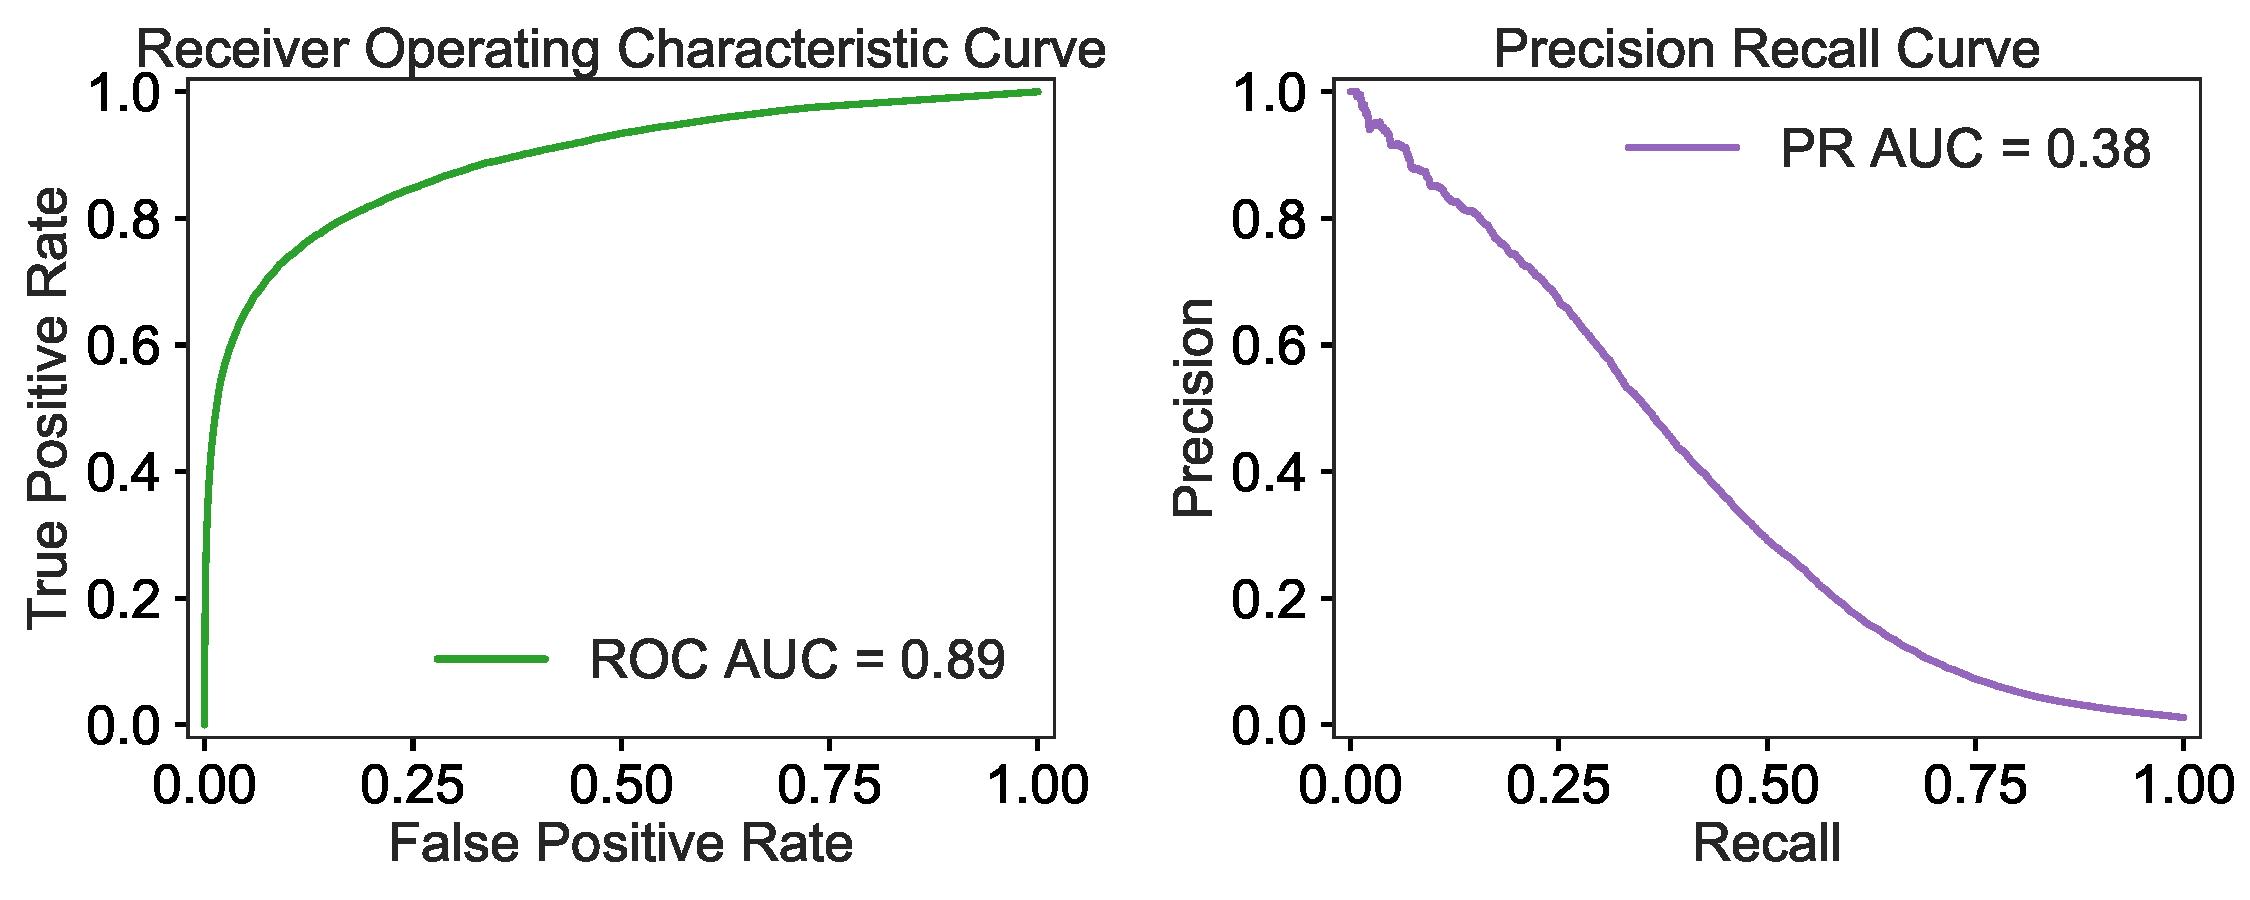
\includegraphics[width=6in]{ET_ROC_PR_plots.pdf}
\end{center}
\caption{\label{fig:ET}
ROC and PR curves for the extremely randomized trees classifier.}
\end{figure}
The ET classifier gives us the best model so far. In the next section, we compare all the models that we have tried in this work and choose the best one.
%%%%%%%%%%%%%%%%%%%%%%%%%
\subsection{Model Comparisons}
\label{sec:modelcomp}
%%%%%%%%%%%%%%%%%%%%%%%%%
We have used logistic regression, naive bayes, random forest, gradient boosting and extra randomized trees classifiers to build a model to predict flight cancellation likelihood. Based on testing the models on the holdout dataset (50$\%$ of the whole data), we found different performance of all models. The results of various evaluation metrics scores are shown in Tab. \ref{tab:modelcomp} for all models. 
\begin{table}[!h]
\centering
\caption{Comparing all models}\label{tab:modelcomp}
\scalebox{1}{
\begin{tabular}{lcccccc}
\toprule
\textbf{Model} & \textbf{PR AUC} & \textbf{ROC AUC} & \textbf{Brier Score} & \textbf{Log Loss} \\
\midrule
\addlinespace
\rc Logistic Regression & \rc 0.51 & \rc 0.50 & \rc 0.01 & \rc 0.69 \\ 
\addlinespace
\addlinespace
Gaussian Naive Bayes & 0.08 & 0.76 & 0.14 & 1.55 \\ 
\addlinespace
\addlinespace
Random Forest & 0.33 & 0.84 & 0.01 & 0.08 \\ 
\addlinespace
\addlinespace
Gradient Boosting & 0.35 & 0.87 & 0.01 & 0.14 \\ 
\addlinespace
\addlinespace
\gc Extremely Randomized Trees & \gc 0.38 & \gc 0.89 & \gc 0.01 & \gc 0.08 \\ 
\addlinespace
\bottomrule \\
\end{tabular}
}
\end{table}
Other than PR AUC and ROC AUC, we also calculated Brier's score (similar to mean square error), and log loss (cost function in logistic regression). These additional metrics are suitable for comparing models when we are interested in predicting probabilities or likelihood. For good models, the values of these two metrics should be close to zero. Table \ref{tab:modelcomp} shows that logistic regression has the highest value for PR AUC, however the ROC AUC is worst. For the Extremely Randomized Trees (ET) model, we get the best results for both PR AUC and ROC AUC. Moreover, both the Brier score and log loss are minimum for ET model. Therefore, the ET model is the best one in this study. We can also look at the ROC and PR curves for all models in Fig. \ref{fig:AllModels} which corroborates the fact that the ET model performs the best.   
\begin{figure}[!h]
\begin{center}
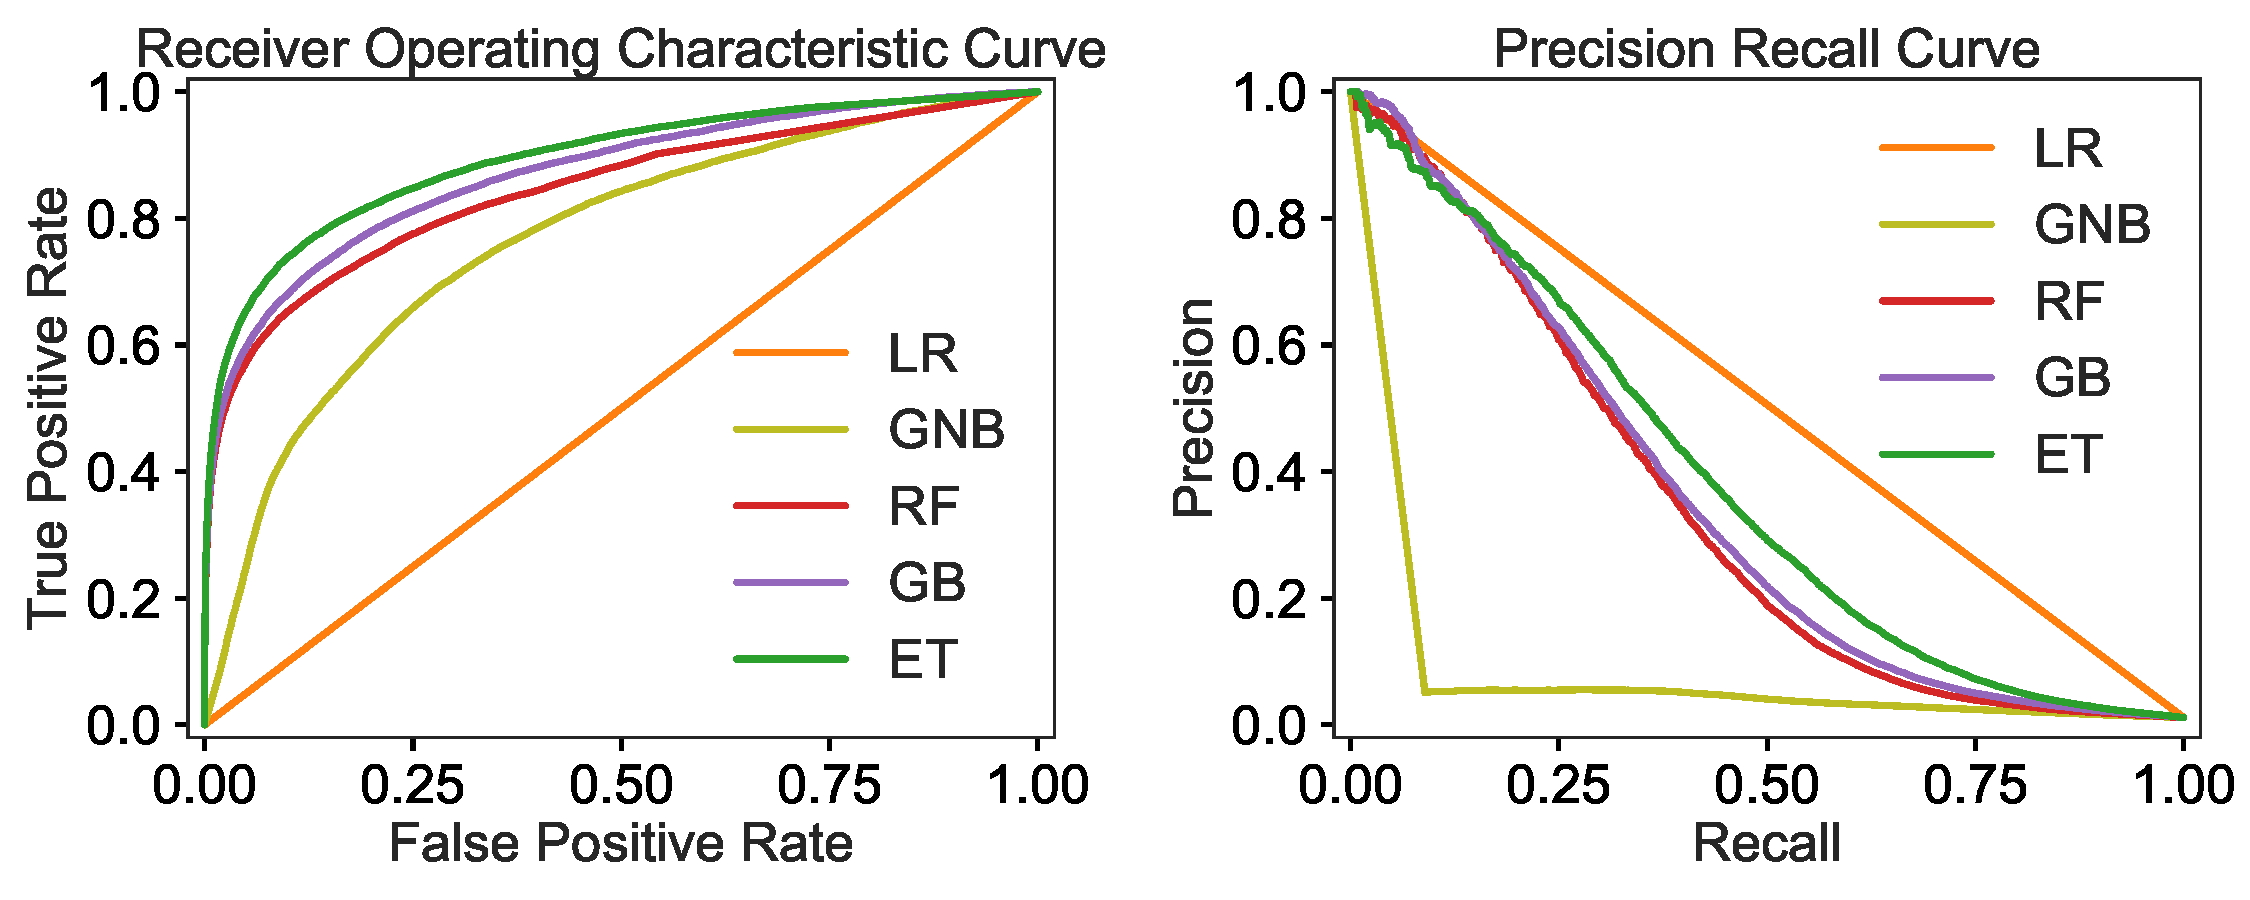
\includegraphics[width=6in]{AllModels_ROC_PR_plots.pdf}
\end{center}
\caption{\label{fig:AllModels}
Comparing ROC and PR curves for all models. LR: Logistic Regression, GNB: Gaussian Naive Bayes, RF: Random Forest, GB: Gradient Boosting, ET: Extremely Randomized Treees.}
\end{figure}



Undersampled test data:


\begin{table}[!h]
\centering
\caption{Comparing all models when test data is undersampled}\label{tab:modelcomp}
\scalebox{1}{
\begin{tabular}{lcccccc}
\toprule
\textbf{Model} & \textbf{PR AUC} & \textbf{ROC AUC} & \textbf{Brier Score} & \textbf{Log Loss} \\
\midrule
\addlinespace
\rc Logistic Regression & \rc 0.75 & \rc 0.50 & \rc 0.5 & \rc 0.69 \\ 
\addlinespace
\addlinespace
Gaussian Naive Bayes & 0.75 & 0.76 & 0.32 & 2.42 \\ 
\addlinespace
\addlinespace
Random Forest & 0.88 & 0.84 & 0.39 & 2.56 \\ 
\addlinespace
\addlinespace
Gradient Boosting & 0.89 & 0.87 & 0.39 & 5.69 \\ 
\addlinespace
\addlinespace
\gc Extremely Randomized Trees & \gc 0.91 & \gc 0.89 & \gc 0.30 & \gc 1.09 \\ 
\addlinespace
\bottomrule \\
\end{tabular}
}
\end{table}

\begin{figure}[!h]
\begin{center}
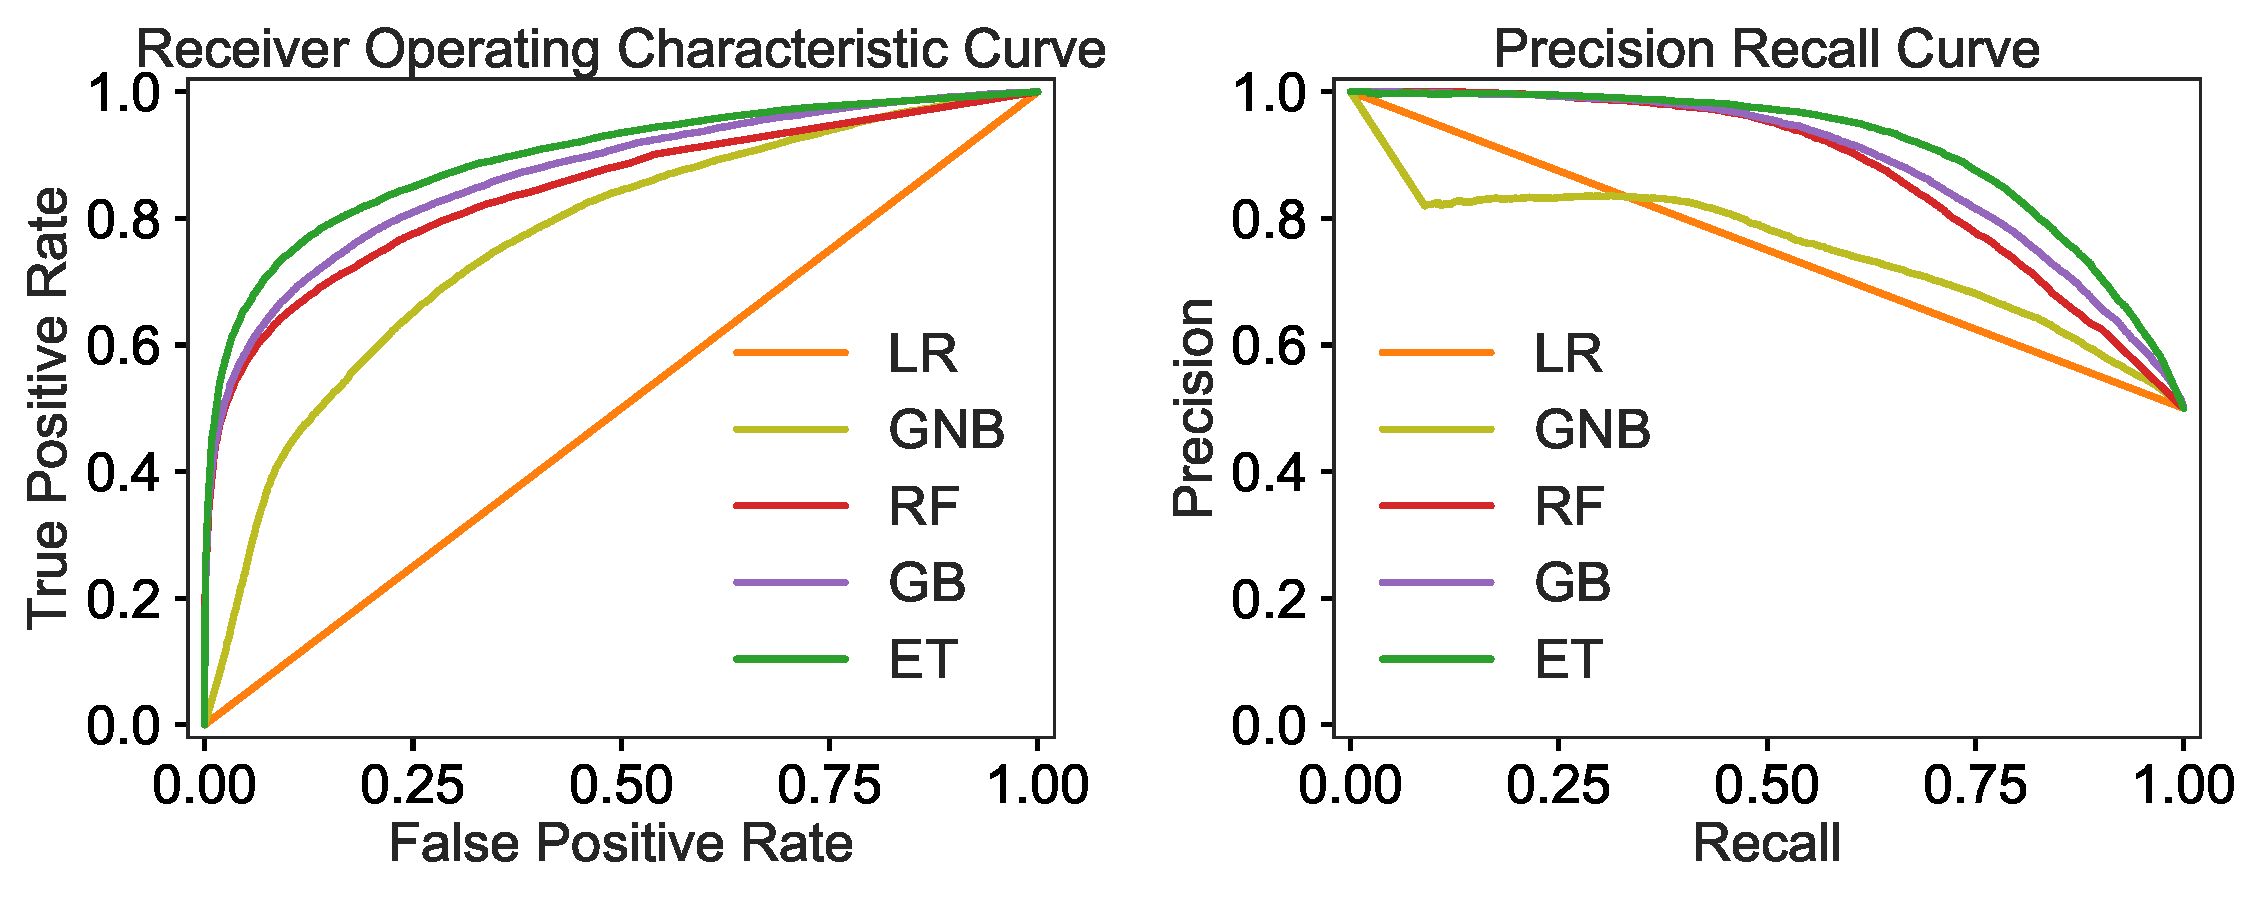
\includegraphics[width=6in]{UndersampledTestDataAllModels_ROC_PR_plots.pdf}
\end{center}
\caption{\label{fig:AllModelsUndersampledTest}
Comparing ROC and PR curves for all models when test data is undersampled. LR: Logistic Regression, GNB: Gaussian Naive Bayes, RF: Random Forest, GB: Gradient Boosting, ET: Extremely Randomized Treees.}
\end{figure}
%%%%%%%%%%%%%%%%%%%%%%%%%
\section{Limitations}
\label{sec:limit}
%%%%%%%%%%%%%%%%%%%%%%%%%
There are some limitations in the data which would reduce the robustness of the machine learning model that we will develop.
\begin{enumerate}
\itemsep0em
\item We have considered only 20 airports in this project due to weather data provider's API restrictions. Though 20 airports broadly cover the whole US, a lot of information will not be learned by the model due to the absence of all airports in the dataset. 
\item The prediction of the model will depend on how good the prediction of the weather is, say after 3 days. In other words. if we want to predict the likelihood of the flight cancellation for a flight which is scheduled after 3 days, we would need to know the weather after 3 days (which we do not know ``accurately" today). This means that the model will predict better if the weather prediction is better or if we are trying to predict the flights not far ago than the scheduled departure.
\item Apart from knowing whether a flight was cancelled, we also have information about the cancellation codes such as A, B, C, D. Most probably these codes correspond to different reasons or factors for cancellation. However, other than just knowing these codes, we do not know the exact meanings of these codes. If the exact meanings were known, we would have built a multi-class classification model. Lack of this information restricts us to develop a binary classifier only.  
\item We found that SunCountry Airline (IATA code: SY) data is missing in the original flight dataset which we acquired from the \href{https://www.transtats.bts.gov/DL_SelectFields.asp?Table_ID=236&DB_Short_Name=On-Time}{Bureau of Transportation Statistics}. We checked for the absence of only this airline from a personal travel experience. It is possible that some other data might also be missing in the original dataset. Therefore, we emphasize that the analysis carried out in this project is only based on the data source that we mentioned here. 
\end{enumerate}
%%%%%%%%%%%%%%%%%%%%%%%%%
\section{Other Data and Future Work}
\label{sec:otherdata}
%%%%%%%%%%%%%%%%%%%%%%%%%
Other than the original flight data, weather data and historical performance data, we can also acquire or feature engineer more datasets which might enhance the predictive power of the machine learning model. Knowing the airport name, we can extract informations such as number of runways, runway length (and width), airport type, airport infrastructure, airport capacity etc.., and create new features. Similarly, knowing the airlines names, we can extract airlines ratings, their stock market performance, their revenue and assets, reputations etc.., and create new fields. We can also get data from social networking sites and news media about the sentiment for each airlines and airports. The sentiment analysis can then be used to create more features. Datasets containing world events such as catastrophic natural destruction, terror attacks, political movement, sport tournaments, etc.. can also be acquired and used to merge with our original datasets. Each one of these ideas can be difficult if the data is not easily accessible. However, we believe that the predictive power of the model will be improved by incorporating these factors.  
%%%%%%%%%%%%%%%%%%%%%%%%%%%%%%%%%
\section{Conclusions}
%%%%%%%%%%%%%%%%%%%%%%%%%%%%%%%%%%%
We have explored the original flight dataset along with the merged weather datasets and engineered historical performance variables, to understand their influence on the flight cancellation rates. Top 20 airports (in terms of the number of flights operating) were considered in this work for the year 2015. The overall cancellation rate was about 1.28$\%$, which is not a large number but that is what makes the project more interesting. We explored 6 types of informations available in the datasets and found that most of them influence cancellation rates. Following is a quick summary of our findings:
\begin{enumerate}
\itemsep0em
\item \textbf{Calendar variables:} Most flights were cancelled in the winter months and least in the falls months. We also found that the cancellations are worst in the end and beginning of a week.
\item \textbf{Airports:} Usually the airports in the east coast had higher cancellation rates as compared to the rest of the nation. LaGuardia and Boston airports topped the list and Salt Lake City and Seattle were bottom in the list of cancellation rates. 
\item \textbf{Airlines:} Regional airlines like Envoy Air and ExpressJet Airlines had higher cancellation rates whereas Delta Airlines, Frontier Airlines and Alaska Airlines performed the best in terms of flight cancellations.
\item \textbf{Flight distance:} The cancellation rates were higher for shorter distance flights and lower for longer distance flights.  
\item \textbf{Weather factors:} Snowy weather is worst and clear sky or even cloudy weather conditions are best in terms of flight cancellation. We also found an increasing trend for cancellation rates as humidity and wind speed increased at both origin and destination airports. Cancellation rates were higher when the  temperatures were less than 40 $^\circ$F, as compared to temperatures greater than 40 $^\circ$F. Finally, we discovered an interesting trend with respect to the wind direction. The cancellation rates were close to 1$\%$ when the wind direction at both origin and destination airports were from East - to - South - to - West. However, we observed a jump in the cancellation rate as the wind direction approached close to North bound. 
\item \textbf{Historical performances:}  In general, we found smaller cancellation rates for flights that got cancelled or diverted less in the last 10-30 days. However, when all the flights got cancelled in the last 10-30 days, the cancellation rate was slightly higher as compared to the cases when all flights were not cancelled. We investigated the cancellation rates for temporary flights (flights that ran only once in last 10-30 days) and found that temporary flights were more likely to cancelled than routine flights. Finally, we also looked at the effect of the history of departure and arrival delays on the cancellation rate of the flight in question and found some interesting trends for shorter range of delays. 
\end{enumerate}
\end{document}
%%%%%%%%%%%%%%%%%%%%%%%%%%%%%%%%%%%%%%%%%%